\documentclass[english,11pt,a4paper]{article}
\usepackage[T1]{fontenc}
\usepackage{graphicx}
\usepackage{mathtools}
\usepackage{amssymb}
\usepackage{amsthm}
\usepackage{thmtools}
\usepackage{xcolor}
\usepackage{nameref}
\usepackage{babel}
\usepackage{authblk}
\usepackage{fourier}
\usepackage{indentfirst}
\usepackage{float}
\usepackage{booktabs}
\usepackage[colorlinks, urlcolor=blue]{hyperref}
\title{Introdução à Neurociência Computacional\\Lista de Exercícios 5}
\author{Paulo R. Sturion}
\begin{document}
	\maketitle
	
	\noindent Todos os códigos escritos para produzir os resultados dos exercícios a seguir estão disponibilizados de forma clara e organizada no repositório Github:
	
	\begin{center}
		\noindent \href{https://github.com/prsturion/intro-computational-neurosciene.git}{https://github.com/prsturion/intro-computational-neuroscience.git} \newline
	\end{center}
	
	\noindent\textbf{Questão 1.}
	
	\noindent\textbf{(a)} Considere $I = 0$. Para este caso, obtenha as equações para as nulclinas de $v$ e $w$ e trace-as no gráfico de $w$ \textit{versus} $v$ (plano de fase).\\
	
	\noindent\textbf{Resposta:}
	
	\noindent\textit{Nulclinas do modelo de FitzHugh--Nagumo para $I=0$.}
	
	\noindent O sistema é
	\[
	\begin{cases}
		\dfrac{dv}{dt} \;=\; v - \dfrac{v^3}{3} - w + I,\\[4pt]
		\dfrac{dw}{dt} \;=\; \phi\,(v + a - b\,w),
	\end{cases}
	\qquad
	\text{com } a=0.7,\; b=0.8,\; \phi=0.08,\; I=0.
	\]
	
	\noindent As \textbf{nulclinas} são obtidas impondo as derivadas a zero:
	
	\[
	\frac{dv}{dt}=0 
	\;\Longrightarrow\;
	v - \frac{v^3}{3} - w = 0
	\;\Longrightarrow\;
	\boxed{\,w = v - \dfrac{v^3}{3}\,}
	\quad \text{(nulclina de $v$).}
	\]
	
	\[
	\frac{dw}{dt}=0 
	\;\Longrightarrow\;
	\phi\,(v + a - b\,w)=0
	\;\Longrightarrow\;
	v + a - b\,w = 0
	\;\Longrightarrow\;
	\boxed{\,w = \dfrac{v + a}{b}\,}
	\quad \text{(nulclina de $w$).}
	\]
	
	\begin{figure}[H]
		\centering
		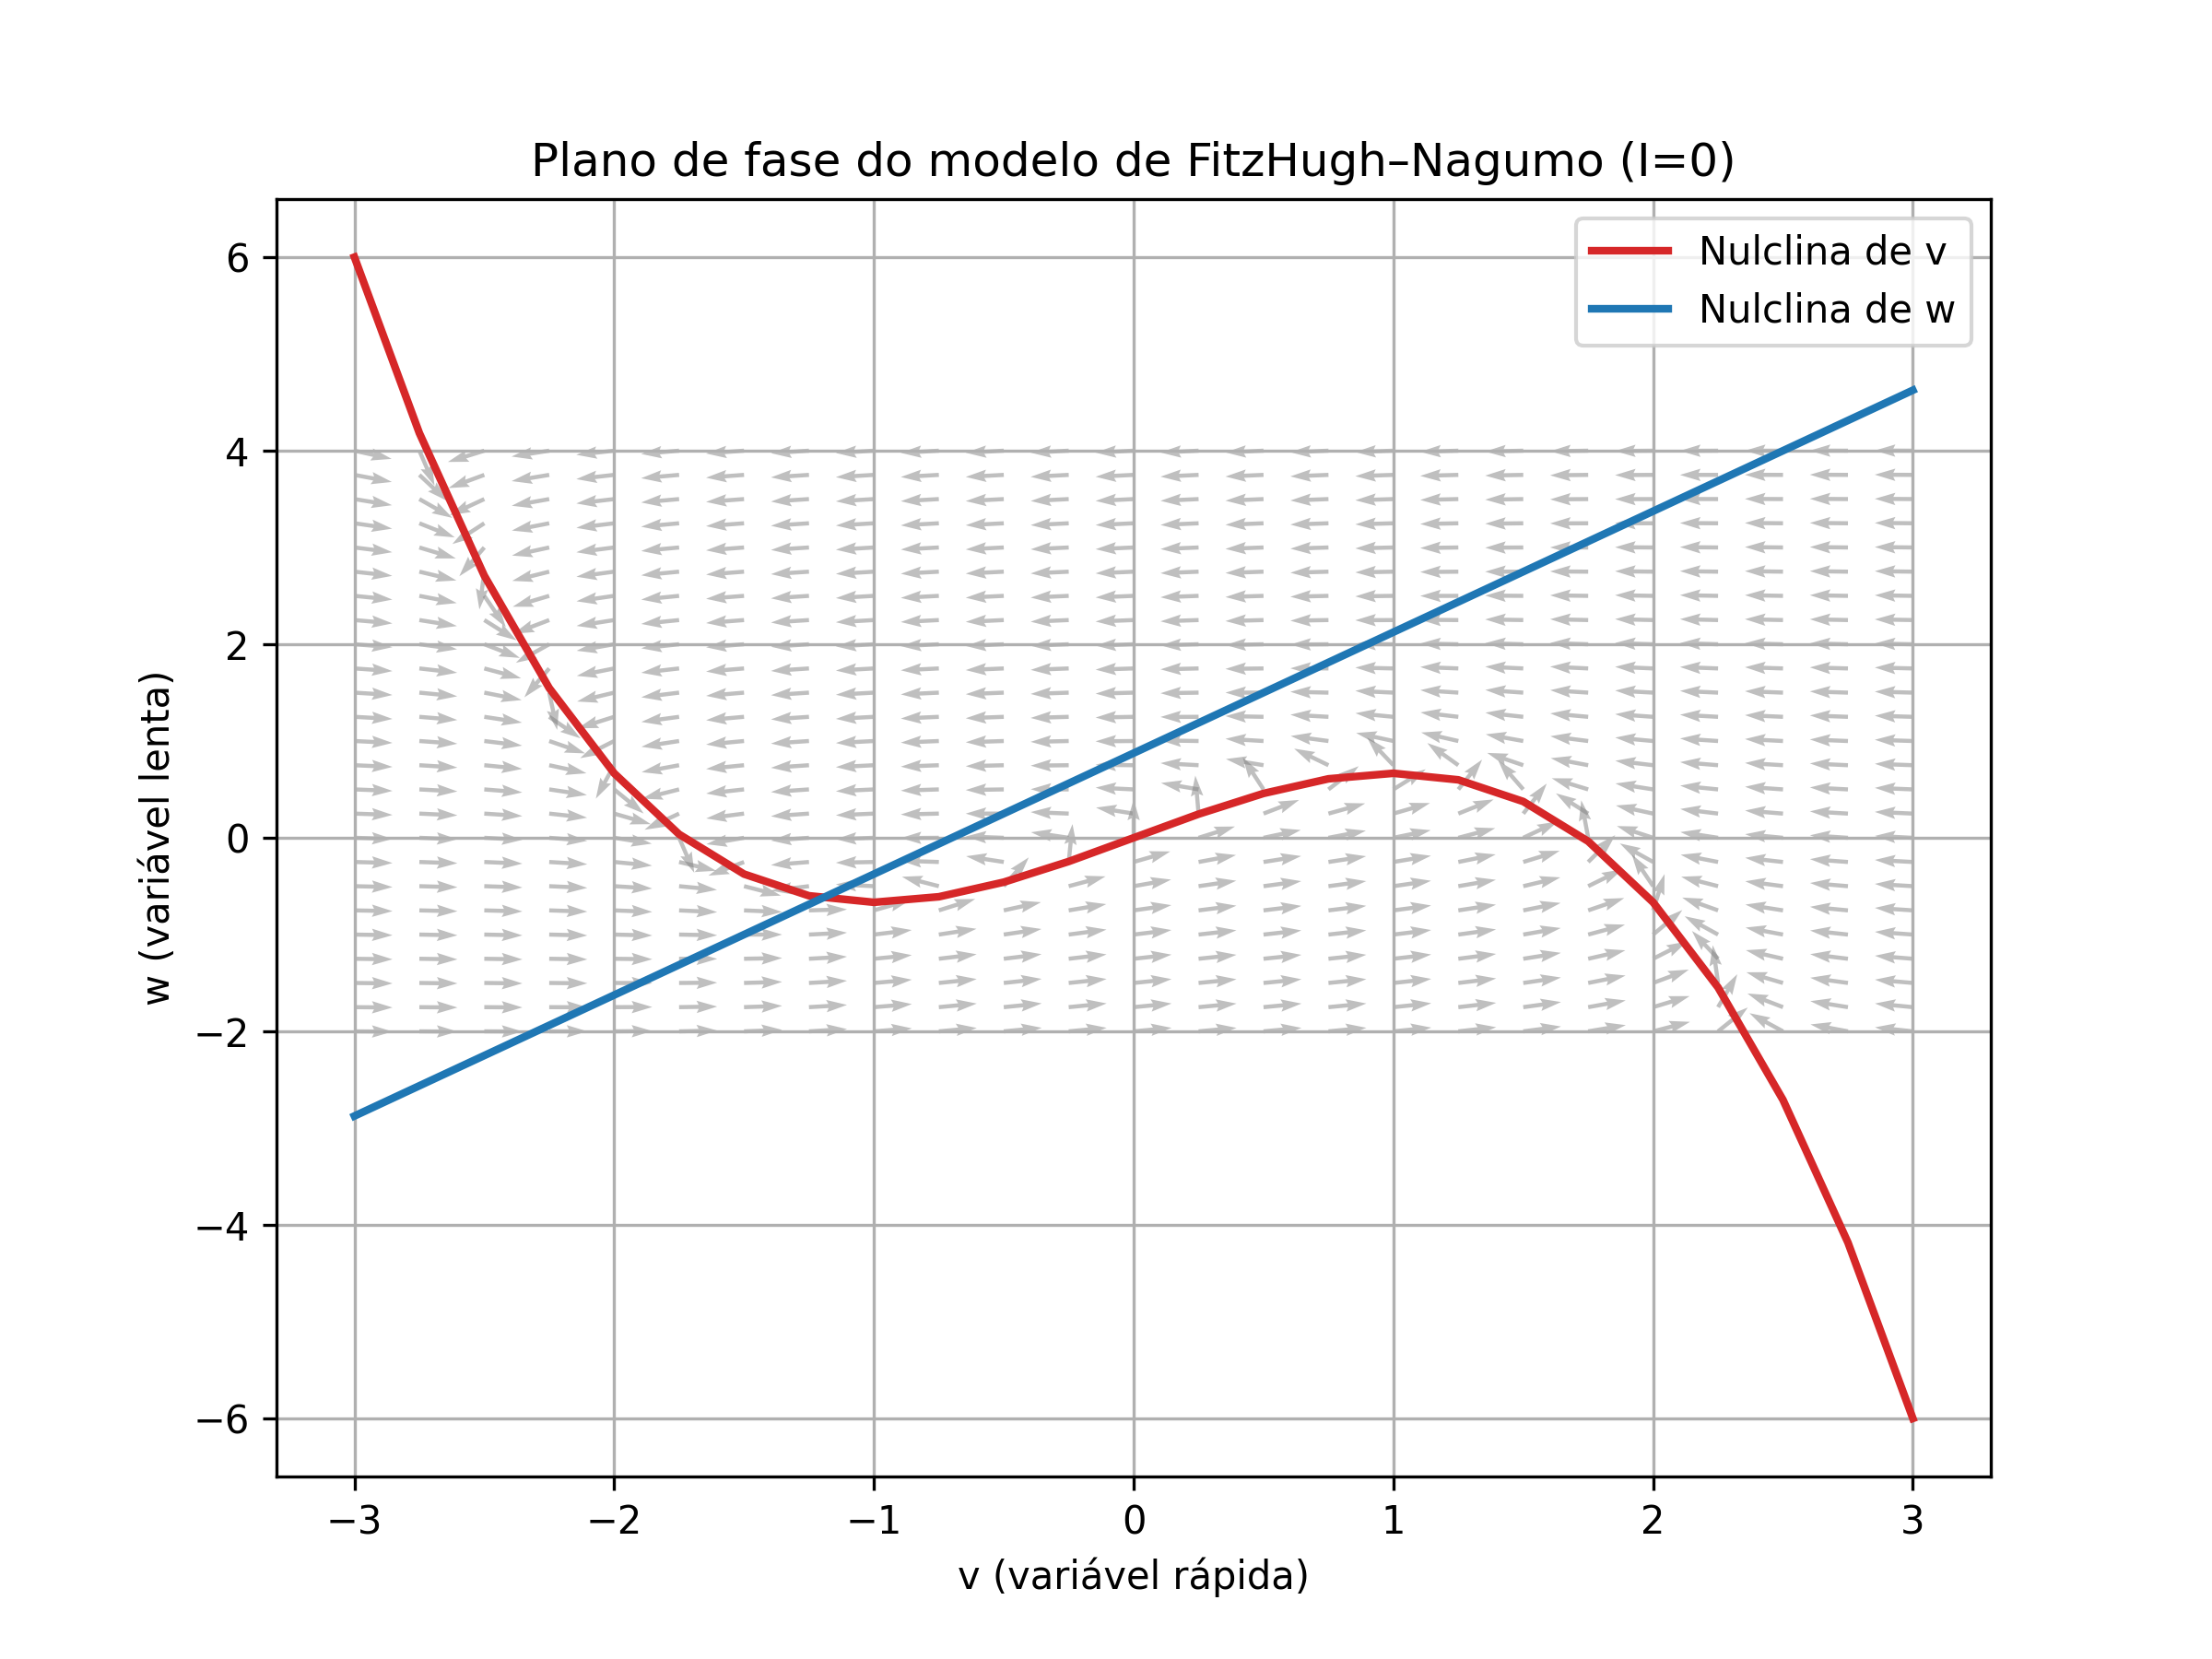
\includegraphics[width=11cm]{../figures/ex_1a.png}
		\caption{Nulclinas do modelo FitzHugh-Nagumo para $I = 0$.}
	\end{figure}
	
	\noindent\textbf{(b)} Determine o(s) ponto(s) de equilíbrio do sistema.\\
	
	\noindent\textbf{Resposta:}
	
	\noindent O(s) ponto(s) de equilíbrio são as interseções das nulclinas, isto é, as soluções de
	\[
	v - \frac{v^3}{3} \;=\; \frac{v + a}{b}.
	\]
	\noindent Equivalentemente,
	\[
	-\frac{b}{3}\,v^3 + (b-1)\,v - a = 0.
	\]
	\noindent (Para $a=0.7$ e $b=0.8$, a raiz real é $v^\ast \approx -1.1994$ e $w^\ast \approx -0.6243$.)\\\\
	
	\noindent\textbf{(c)} Linearize o sistema de equações (1) e (2) para determinar a natureza do(s) ponto(s) de equilíbrio. Para fazer isso, seja $(v^*, w^*)$ um ponto de equilíbrio do sistema. Considere pequenas perturbações em torno deste ponto de equilíbrio: $v = v^* + \delta v$ e $w = w^* + \delta w$. Substitua estas expressões no sistema de equações e despreze os termos de ordem quadrática ou superior em $\delta v$ e $\delta w$. Você deve ficar com um sistema do tipo:
	\[
	\frac{d(\delta v)}{dt} = p\,\delta v + q\,\delta w
	\]
	\[
	\frac{d(\delta w)}{dt} = r\,\delta v + s\,\delta w,
	\]
	que pode ser escrito na forma matricial,
	\[
	\begin{bmatrix}
		d(\delta v)/dt \\[4pt]
		d(\delta w)/dt
	\end{bmatrix}
	=
	\begin{bmatrix}
		p & q \\[4pt]
		r & s
	\end{bmatrix}
	\begin{bmatrix}
		\delta v \\[4pt]
		\delta w
	\end{bmatrix}.
	\]
	
	A matriz $\begin{bmatrix} p & q \\ r & s \end{bmatrix}$ é chamada de \textit{matriz jacobiana} do sistema no ponto de equilíbrio $(v^*, w^*)$. É importante notar que cada ponto de equilíbrio tem uma matriz jacobiana diferente. Quais os valores de $p$, $q$, $r$ e $s$ para cada um dos pontos de equilíbrio do sistema?\\
	
	\noindent\textbf{Resposta:}
	
	\noindent\textit{Linearização e matriz jacobiana no(s) ponto(s) de equilíbrio.}
	
	\noindent Considere o sistema de FitzHugh--Nagumo
	\[
	\begin{cases}
		\dfrac{dv}{dt} = f(v,w) \;=\; v - \dfrac{v^{3}}{3} - w + I,\\[4pt]
		\dfrac{dw}{dt} = g(v,w) \;=\; \phi\,(v + a - b\,w),
	\end{cases}
	\]
	e seja \((v^\ast,w^\ast)\) um ponto de equilíbrio, i.e.,
	\[
	f(v^\ast,w^\ast)=0, \qquad g(v^\ast,w^\ast)=0.
	\]
	
	\noindent Introduza pequenas perturbações em torno do equilíbrio:
	\[
	v(t)=v^\ast+\delta v(t), \qquad w(t)=w^\ast+\delta w(t),
	\]
	e faça a expansão de Taylor de primeira ordem (desprezando termos quadráticos e de ordem superior):
	\[
	\begin{aligned}
		\dfrac{d(\delta v)}{dt}
		&= f_v(v^\ast,w^\ast)\,\delta v \;+\; f_w(v^\ast,w^\ast)\,\delta w,\\[4pt]
		\dfrac{d(\delta w)}{dt}
		&= g_v(v^\ast,w^\ast)\,\delta v \;+\; g_w(v^\ast,w^\ast)\,\delta w,
	\end{aligned}
	\]
	onde \(f_v=\partial f/\partial v\), \(f_w=\partial f/\partial w\), \(g_v=\partial g/\partial v\) e \(g_w=\partial g/\partial w\).
	
	\noindent Logo, o sistema linearizado assume a forma solicitada:
	\[
	\dfrac{d(\delta v)}{dt} = p\,\delta v + q\,\delta w, 
	\qquad
	\dfrac{d(\delta w)}{dt} = r\,\delta v + s\,\delta w,
	\]
	com
	\[
	\boxed{
		\begin{aligned}
			p &= f_v(v^\ast,w^\ast) \;=\; 1 - (v^\ast)^2,\\[2pt]
			q &= f_w(v^\ast,w^\ast) \;=\; -1,\\[2pt]
			r &= g_v(v^\ast,w^\ast) \;=\; \phi,\\[2pt]
			s &= g_w(v^\ast,w^\ast) \;=\; -\phi\,b.
	\end{aligned}}
	\]
	
	\noindent Em forma matricial:
	\[
	\begin{bmatrix}
		\dfrac{d(\delta v)}{dt}\\[2pt]
		\dfrac{d(\delta w)}{dt}
	\end{bmatrix}
	=
	\underbrace{\begin{bmatrix}
			p & q\\
			r & s
	\end{bmatrix}}_{\displaystyle J(v^\ast,w^\ast)}
	\begin{bmatrix}
		\delta v\\[2pt]
		\delta w
	\end{bmatrix}
	\;=\;
	\begin{bmatrix}
		1-(v^\ast)^2 & -1\\
		\phi & -\phi b
	\end{bmatrix}
	\begin{bmatrix}
		\delta v\\[2pt]
		\delta w
	\end{bmatrix}.
	\]
	
	\noindent Para o conjunto de parâmetros do enunciado \((a=0{,}7,\; b=0{,}8,\; \phi=0{,}08)\) e \(I=0\), o equilíbrio real é
	\[
	v^\ast \approx -1{,}1994,\qquad w^\ast = v^\ast - \frac{(v^\ast)^3}{3} \approx -0{,}6243,
	\]
	de modo que
	\[
	\boxed{\,p \approx -0{,}4386,\quad q=-1,\quad r=0{,}08,\quad s=-0{,}064.\,}
	\]
	
	
	\noindent\textbf{(d)} Para analisar o tipo de estabilidade de um dado ponto de equilíbrio, é necessário determinar os autovalores da sua matriz jacobiana. Os livros de texto de álgebra linear ensinam como calcular os autovalores e os autovetores de uma matriz arbitrária. Seja uma matriz $L = \begin{bmatrix} p & q \\ r & s \end{bmatrix}$. Para encontrar os seus autovalores, deve-se resolver a chamada \textit{equação característica}:
	\[
	\det
	\begin{bmatrix}
		p - \lambda & q \\
		r & s - \lambda
	\end{bmatrix}
	= 0.
	\]
	
	Esta equação pode ser posta na forma polinomial $(p - \lambda)(s - \lambda) - qr = 0$, ou,
	\[
	\lambda^2 - \tau \lambda + \Delta = 0,
	\]
	onde
	\[
	\tau = \mathrm{Tr}\,L = p + s
	\quad \text{e} \quad
	\Delta = \det L = ps - qr
	\]
	são, respectivamente, o traço e o determinante da matriz $L$. A forma polinomial quadrática acima tem duas soluções da forma:
	\[
	\lambda_1 = \frac{\tau + \sqrt{\tau^2 - 4\Delta}}{2}
	\quad \text{e} \quad
	\lambda_2 = \frac{\tau - \sqrt{\tau^2 - 4\Delta}}{2},
	\]
	que são números reais (quando $\tau^2 - 4\Delta \geq 0$) ou complexos conjugados (quando $\tau^2 - 4\Delta < 0$). Calcule os autovalores da matriz jacobiana para o(s) ponto(s) de equilíbrio do sistema.\\
	
	\noindent\textbf{Resposta:}
	
	\noindent\textit{Autovalores da matriz jacobiana no(s) ponto(s) de equilíbrio.}
	
	\noindent Seja a matriz jacobiana no equilíbrio \((v^\ast,w^\ast)\)
	\[
	J(v^\ast,w^\ast)=
	\begin{bmatrix}
		p & q\\
		r & s
	\end{bmatrix}
	=
	\begin{bmatrix}
		1-(v^\ast)^2 & -1\\
		\phi & -\phi b
	\end{bmatrix}.
	\]
	
	\noindent Os autovalores \(\lambda\) satisfazem a equação característica
	\[
	\det\!\begin{bmatrix}
		p-\lambda & q\\
		r & s-\lambda
	\end{bmatrix}=0
	\;\;\Longleftrightarrow\;\;
	\lambda^2 - \tau\,\lambda + \Delta = 0,
	\]
	onde
	\[
	\tau=\operatorname{Tr}J = p+s, 
	\qquad 
	\Delta=\det J = ps - qr .
	\]
	Logo,
	\[
	\boxed{\;\lambda_{1,2}=\frac{\tau \pm \sqrt{\tau^{2}-4\Delta}}{2}\; }.
	\]
	
	\noindent Para os parâmetros do enunciado e \(I=0\), o(s) equilíbrio(s) \((v^\ast,w^\ast)\) são dados pela interseção das nulclinas
	\(
	w = v - \frac{v^3}{3}
	\)
	e
	\(
	w = \frac{v+a}{b}
	\).
	Nesse caso há uma única raiz real \(v^\ast \approx -1{,}1994\) e 
	\(
	w^\ast = v^\ast - \frac{(v^\ast)^3}{3} \approx -0{,}6243.
	\)
	
	\noindent Substituindo em \(p,q,r,s\):
	\[
	p = 1-(v^\ast)^2 \approx -0{,}4386,\quad
	q=-1,\quad
	r=\phi=0{,}08,\quad
	s=-\phi b=-0{,}064.
	\]
	Assim,
	\[
	\tau=p+s \approx -0{,}50258,
	\qquad
	\Delta=ps-qr \approx 0{,}10807,
	\]
	e
	\[
	\tau^2-4\Delta \approx -0{,}17969 < 0,
	\]
	o que implica um par complexo conjugado com parte real negativa:
	\[
	\boxed{\;
		\lambda_{1,2} \approx -0{,}25129 \;\pm\; 0{,}21195\,i
		\;}
	\]\\
	
	
	\noindent\textbf{(e)} Em geral, uma matriz $2 \times 2$ tem dois autovalores com autovetores distintos,
	\[
	v_1 =
	\begin{bmatrix}
		v_{11} \\
		v_{12}
	\end{bmatrix}
	\quad \text{e} \quad
	v_2 =
	\begin{bmatrix}
		v_{21} \\
		v_{22}
	\end{bmatrix}.
	\]
	Nesses casos, a solução geral do sistema linearizado é da forma:
	\[
	\begin{bmatrix}
		\delta v \\
		\delta w
	\end{bmatrix}
	= c_1 e^{\lambda_1 t} v_1 + c_2 e^{\lambda_2 t} v_2,
	\]
	onde $c_1$ e $c_2$ são constantes que dependem das condições iniciais. Quando os dois autovalores são reais e negativos, ou complexos com as partes reais negativas, a equação acima implica que as perturbações $\delta v$ e $\delta w$ decaem para zero com o tempo e, portanto, o ponto de equilíbrio $(v^*, w^*)$ é assintoticamente estável. Quando pelo menos um dos autovalores é real e positivo, ou é complexo com a parte real positiva, então o ponto de equilíbrio $(v^*, w^*)$ é instável. Determine a estabilidade ou a instabilidade do(s) ponto(s) de equilíbrio do sistema.
	
	\noindent\textbf{Resposta:}
	
	\noindent\textit{Estabilidade via solução geral do sistema linearizado.}
	
	\noindent Para o sistema linearizado no equilíbrio \((v^\ast,w^\ast)\),
	\[
	\frac{d}{dt}\begin{bmatrix}\delta v\\ \delta w\end{bmatrix}
	= J(v^\ast,w^\ast)\begin{bmatrix}\delta v\\ \delta w\end{bmatrix},
	\qquad
	J=\begin{bmatrix}p & q\\ r & s\end{bmatrix},
	\]
	se \(J\) tiver dois autovalores \(\lambda_1,\lambda_2\) com autovetores \(\nu_1,\nu_2\) linearmente independentes, a solução geral é
	\[
	\begin{bmatrix}\delta v(t)\\ \delta w(t)\end{bmatrix}
	= c_1 e^{\lambda_1 t}\,\nu_1 \;+\; c_2 e^{\lambda_2 t}\,\nu_2,
	\]
	onde \(c_1,c_2\) dependem das condições iniciais.
	
	\medskip
	\noindent Critérios de estabilidade (2D):
	\[
	\lambda_{1,2}=\frac{\tau\pm\sqrt{\tau^2-4\Delta}}{2}, 
	\qquad \tau=\operatorname{Tr}J=p+s,\quad \Delta=\det J=ps-qr.
	\]
	\[
	\begin{array}{lcl}
		\text{(i)} & \Re(\lambda_1),\Re(\lambda_2)<0 &\Rightarrow\ \text{equilíbrio assintoticamente estável;}\\
		\text{(ii)} & \exists\,\lambda\ \text{com }\Re(\lambda)>0 &\Rightarrow\ \text{equilíbrio instável;}\\
		\text{(iii)} & \Re(\lambda_1)=\Re(\lambda_2)=0 &\Rightarrow\ \text{caso limite (não conclui estabilidade).}
	\end{array}
	\]
	
	\medskip
	\noindent No nosso caso, os autovalores formam um par complexo conjugado com parte real negativa:
	\[
	\lambda_{1,2}\approx -0{,}2513 \pm 0{,}2120\,i.
	\]
	Como \(\Re(\lambda_{1,2})<0\), segue que
	\[
	\boxed{\text{o ponto de equilíbrio é \textbf{estável}.}}
	\]
	
	
	
	\noindent\textbf{(f)} Os autovalores da matriz jacobiana de um ponto de equilíbrio também determinam a maneira como o sistema converge (ou diverge) para o (ou do) ponto de equilíbrio nas suas vizinhanças no plano de fase. Há três tipos de convergência (ou divergência), correspondendo a três tipos de pontos de equilíbrio chamados na literatura de \textit{nó}, \textit{sela} e \textit{foco} (ou \textit{espiral}). Um nó ocorre quando os autovalores são reais e do mesmo sinal. Se eles forem negativos, o nó é estável, e se eles forem positivos o nó é instável. Um ponto de sela ocorre quando os autovalores são reais e de sinais opostos. Os pontos de sela são sempre instáveis. Um foco ocorre quando os autovalores são complexos conjugados. Quando as suas partes reais são negativas, o foco é estável, e quando as suas partes reais são positivas o foco é instável. A Figura~1 ilustra os tipos de convergência (divergência).
	
	Quando os dois autovalores forem puramente imaginários, isto é, forem números complexos com suas partes reais nulas, então o ponto de equilíbrio é chamado de \textit{centro}. Neste caso, as trajetórias do sistema são órbitas fechadas em torno do ponto de equilíbrio (veja a Figura~2).
	
	Um centro é um ponto de equilíbrio chamado de \textit{neutralmente estável}. Todos os tipos de estabilidade de um ponto de equilíbrio podem ser mostrados em um gráfico de $\tau \times \Delta$ (o traço da matriz jacobiana \textit{versus} o seu determinante). A Figura~3 ilustra isso.
	
	Na Figura~3, a linha indicada como bifurcação sela-nó corresponde à região do plano $\tau \times \Delta$ para a qual um dos autovalores é zero; o equilíbrio ao longo dessa linha é de um tipo misto (veja a ilustração do meio na Figura~14 nas notas de aula de análise qualitativa do modelo de Hodgkin-Huxley) chamado de \textit{equilíbrio sela-nó}. Já a linha indicada na Figura~3 como bifurcação de Andronov-Hopf corresponde à região do plano para a qual os pontos de equilíbrio são centros. Uma bifurcação de Andronov-Hopf corresponde à transição de um foco estável para um foco instável ou vice-versa. Determine o tipo de convergência (divergência) do sistema para o(s) seu(s) ponto(s) de equilíbrio nas vizinhanças desse(s) ponto(s).\\
	
	\noindent\textbf{Resposta:}
	
	\noindent\textit{Tipo de convergência/divergência a partir dos autovalores.}
	
	\noindent Para a matriz jacobiana no equilíbrio \((v^\ast,w^\ast)\),
	\[
	J=\begin{bmatrix}p & q\\ r & s\end{bmatrix},
	\qquad
	\lambda_{1,2}=\frac{\tau\pm\sqrt{\tau^2-4\Delta}}{2},
	\quad
	\tau=\mathrm{Tr}\,J=p+s,\ \ \Delta=\det J=ps-qr .
	\]
	
	\noindent Regras de classificação (plano \(\tau\times\Delta\)):
	\[
	\begin{array}{ll}
		\text{sela} & \Leftrightarrow\ \Delta<0;\\[2pt]
		\text{nó estável/instável} & \Leftrightarrow\ \Delta>0,\ \tau^2-4\Delta\ge 0,\ \text{com } \tau<0/\tau>0;\\[2pt]
		\text{foco estável/instável} & \Leftrightarrow\ \Delta>0,\ \tau^2-4\Delta<0,\ \text{com } \tau<0/\tau>0;\\[2pt]
		\text{centro (neutro)} & \Leftrightarrow\ \Delta>0,\ \tau=0\ (\Rightarrow\ \lambda=\pm i\sqrt{\Delta}).
	\end{array}
	\]
	
	\noindent Para os parâmetros do enunciado \((a=0{,}7,\ b=0{,}8,\ \phi=0{,}08,\ I=0)\), do item (d) obtemos no único equilíbrio:
	\[
	\tau \approx -0{,}5026,\qquad \Delta \approx 0{,}1081,\qquad \tau^2-4\Delta<0.
	\]
	Logo, \(\lambda_{1,2}\) formam um par complexo conjugado com parte real negativa:
	\[
	\lambda_{1,2}\approx -0{,}2513 \pm 0{,}2120\,i .
	\]
	
	\noindent \textbf{Conclusão.} Como \(\Delta>0\), \(\tau<0\) e \(\tau^2-4\Delta<0\), o equilíbrio é um
	\[
	\boxed{\text{\textbf{foco estável} (espiral estável).}}
	\]\\
	
	\noindent\textbf{(g)} Se os autovalores da matriz jacobiana de um ponto de equilíbrio forem reais e não nulos, ou complexos conjugados com a parte real diferente de zero, então o ponto de equilíbrio é chamado de \textit{hiperbólico} (estável ou instável). A importância dos pontos de equilíbrio hiperbólicos é que, segundo o teorema de Hartman-Grobman (veja o livro de Izhikevich nas referências), o seu tipo de estabilidade é robusto, isto é, o tipo de estabilidade determinado pela linearização do sistema (como você fez no item (c) e (d) acima) mantém-se para o sistema não linear sem desprezar os termos de ordem superior em $\delta v$ e $\delta w$. Dizemos que a dinâmica do sistema não linear nas vizinhanças de um ponto de equilíbrio hiperbólico é \textit{topologicamente equivalente} à dinâmica da sua versão linearizada. Isto quer dizer que os termos de ordem superior que foram desprezados na análise linearizada do sistema não desempenham qualquer papel qualitativo na sua dinâmica. Em linguagem mais matemática, tal caso existe um \textit{homeomorfismo} (uma deformação contínua com inversa contínua) que mapeia o plano de fase do sistema linearizado no plano de fase do sistema não linear. As trajetórias e as direções dos vetores são preservadas quando se mapeia um diagrama no outro. Em uma linguagem mais livre, dois planos de fase topologicamente equivalentes são como versões distorcidas um do outro. Eles podem estar dobrados ou esticados (mas não rasgados), de maneira que trajetórias fechadas em um plano continuam fechadas no outro. Quando um ponto de equilíbrio tem autovalores reais nulos, ou complexos conjugados com a parte real nula, ele é chamado de \textit{não-hiperbólico}. Os pontos de equilíbrio não-hiperbólicos não são robustos e a técnica de linearização não pode determinar o seu tipo de estabilidade no caso geral. O aparecimento de autovalores reais nulos ou de complexos conjugados com a parte real nula ocorre quando o ponto de equilíbrio passa por uma bifurcação (veja o diagrama da Figura~3). Determine se o(s) ponto(s) de equilíbrio do sistema é(são) hiperbólico(s) ou não-hiperbólico(s).\\
	
	\noindent\textbf{Resposta:}
	
	\noindent\textit{Ponto(s) de equilíbrio hiperbólico(s) ou não-hiperbólico(s).}
	
	\noindent Seja a matriz jacobiana no equilíbrio \((v^\ast,w^\ast)\)
	\[
	J=\begin{bmatrix}p & q\\ r & s\end{bmatrix}, 
	\qquad 
	\lambda_{1,2}=\frac{\tau\pm\sqrt{\tau^2-4\Delta}}{2},
	\quad 
	\tau=\mathrm{Tr}\,J=p+s,\ \ \Delta=\det J=ps-qr .
	\]
	
	\noindent \textbf{Definição.} Um ponto de equilíbrio é \emph{hiperbólico} se \(\Re(\lambda_1)\neq 0\) e \(\Re(\lambda_2)\neq 0\). 
	Equivalências úteis em dimensão \(2\):
	\[
	\begin{array}{ll}
		\text{não-hiperbólico} & \Leftrightarrow\ \Delta=0\ \ (\text{algum } \lambda=0)\ \ \text{ou}\ \ \tau=0\ \text{e}\ \Delta>0\ (\lambda=\pm i\sqrt{\Delta});\\[2pt]
		\text{hiperbólico} & \Leftrightarrow\ \Delta\neq 0\ \text{ e, no caso complexo, } \tau\neq 0\ (\Re[\lambda]=\tau/2\neq 0).
	\end{array}
	\]
	
	\noindent Para os parâmetros do problema \((a=0{,}7,\ b=0{,}8,\ \phi=0{,}08,\ I=0)\), do item (d) obtivemos, no único equilíbrio,
	\[
	\tau \approx -0{,}5026,\qquad \Delta \approx 0{,}1081,\qquad 
	\lambda_{1,2}\approx -0{,}2513 \pm 0{,}2120\,i .
	\]
	Como \(\Delta\neq 0\) e \(\tau\neq 0\), tem-se \(\Re(\lambda_{1,2})=\tau/2\neq 0\).
	
	\medskip
	\noindent \(\Rightarrow\) \(\boxed{\text{O ponto de equilíbrio é \textbf{hiperbólico}.}}\)
	
	
	\noindent\textbf{(h)} Construa um programa que resolva o sistema de equações do modelo de FitzHugh-Nagumo com $I = 0$ pelo método de Euler com passo de tempo $h = 0{,}001$ ou pelo método de Runge-Kutta de 4ª ordem com um passo de tempo maior. Use seu programa para simular o efeito de um pulso instantâneo de corrente $I(t) = Q\delta(t)$ (com $Q > 0$) sobre o modelo. Para simular isso, basta fazer o valor inicial de $v$ na simulação ($v(0)$) ser diferente do valor de equilíbrio $v^*$ obtido no item (b) (o valor inicial de $w(0)$ pode ser $w^*$). Use os seguintes valores de $v(0)$: $-0{,}8$, $-0{,}65$, $-0{,}64$ e $-0{,}6$. Faça as simulações durarem de $t = 0$ a $t = 40$ (lembre-se que as variáveis são adimensionais) e produza três gráficos com ele: (i) um gráfico com as curvas de $v \times t$ para os quatro valores de $v(0)$ superpostas (cada curva indicada por uma cor ou símbolo diferente); (ii) um gráfico com as curvas de $w \times t$ para os quatro valores de $v(0)$ superpostas (cada curva indicada por uma cor ou símbolo diferente); (iii) um gráfico do plano de fase $w \times v$ mostrando as nulclinas de $v$ e $w$ (em cores ou símbolos diferentes) e as trajetórias correspondentes aos quatro casos simulados (também em cores ou símbolos diferentes).\\
	
	\noindent\textbf{Respota:}
	
	\begin{figure}[H]
		\centering
		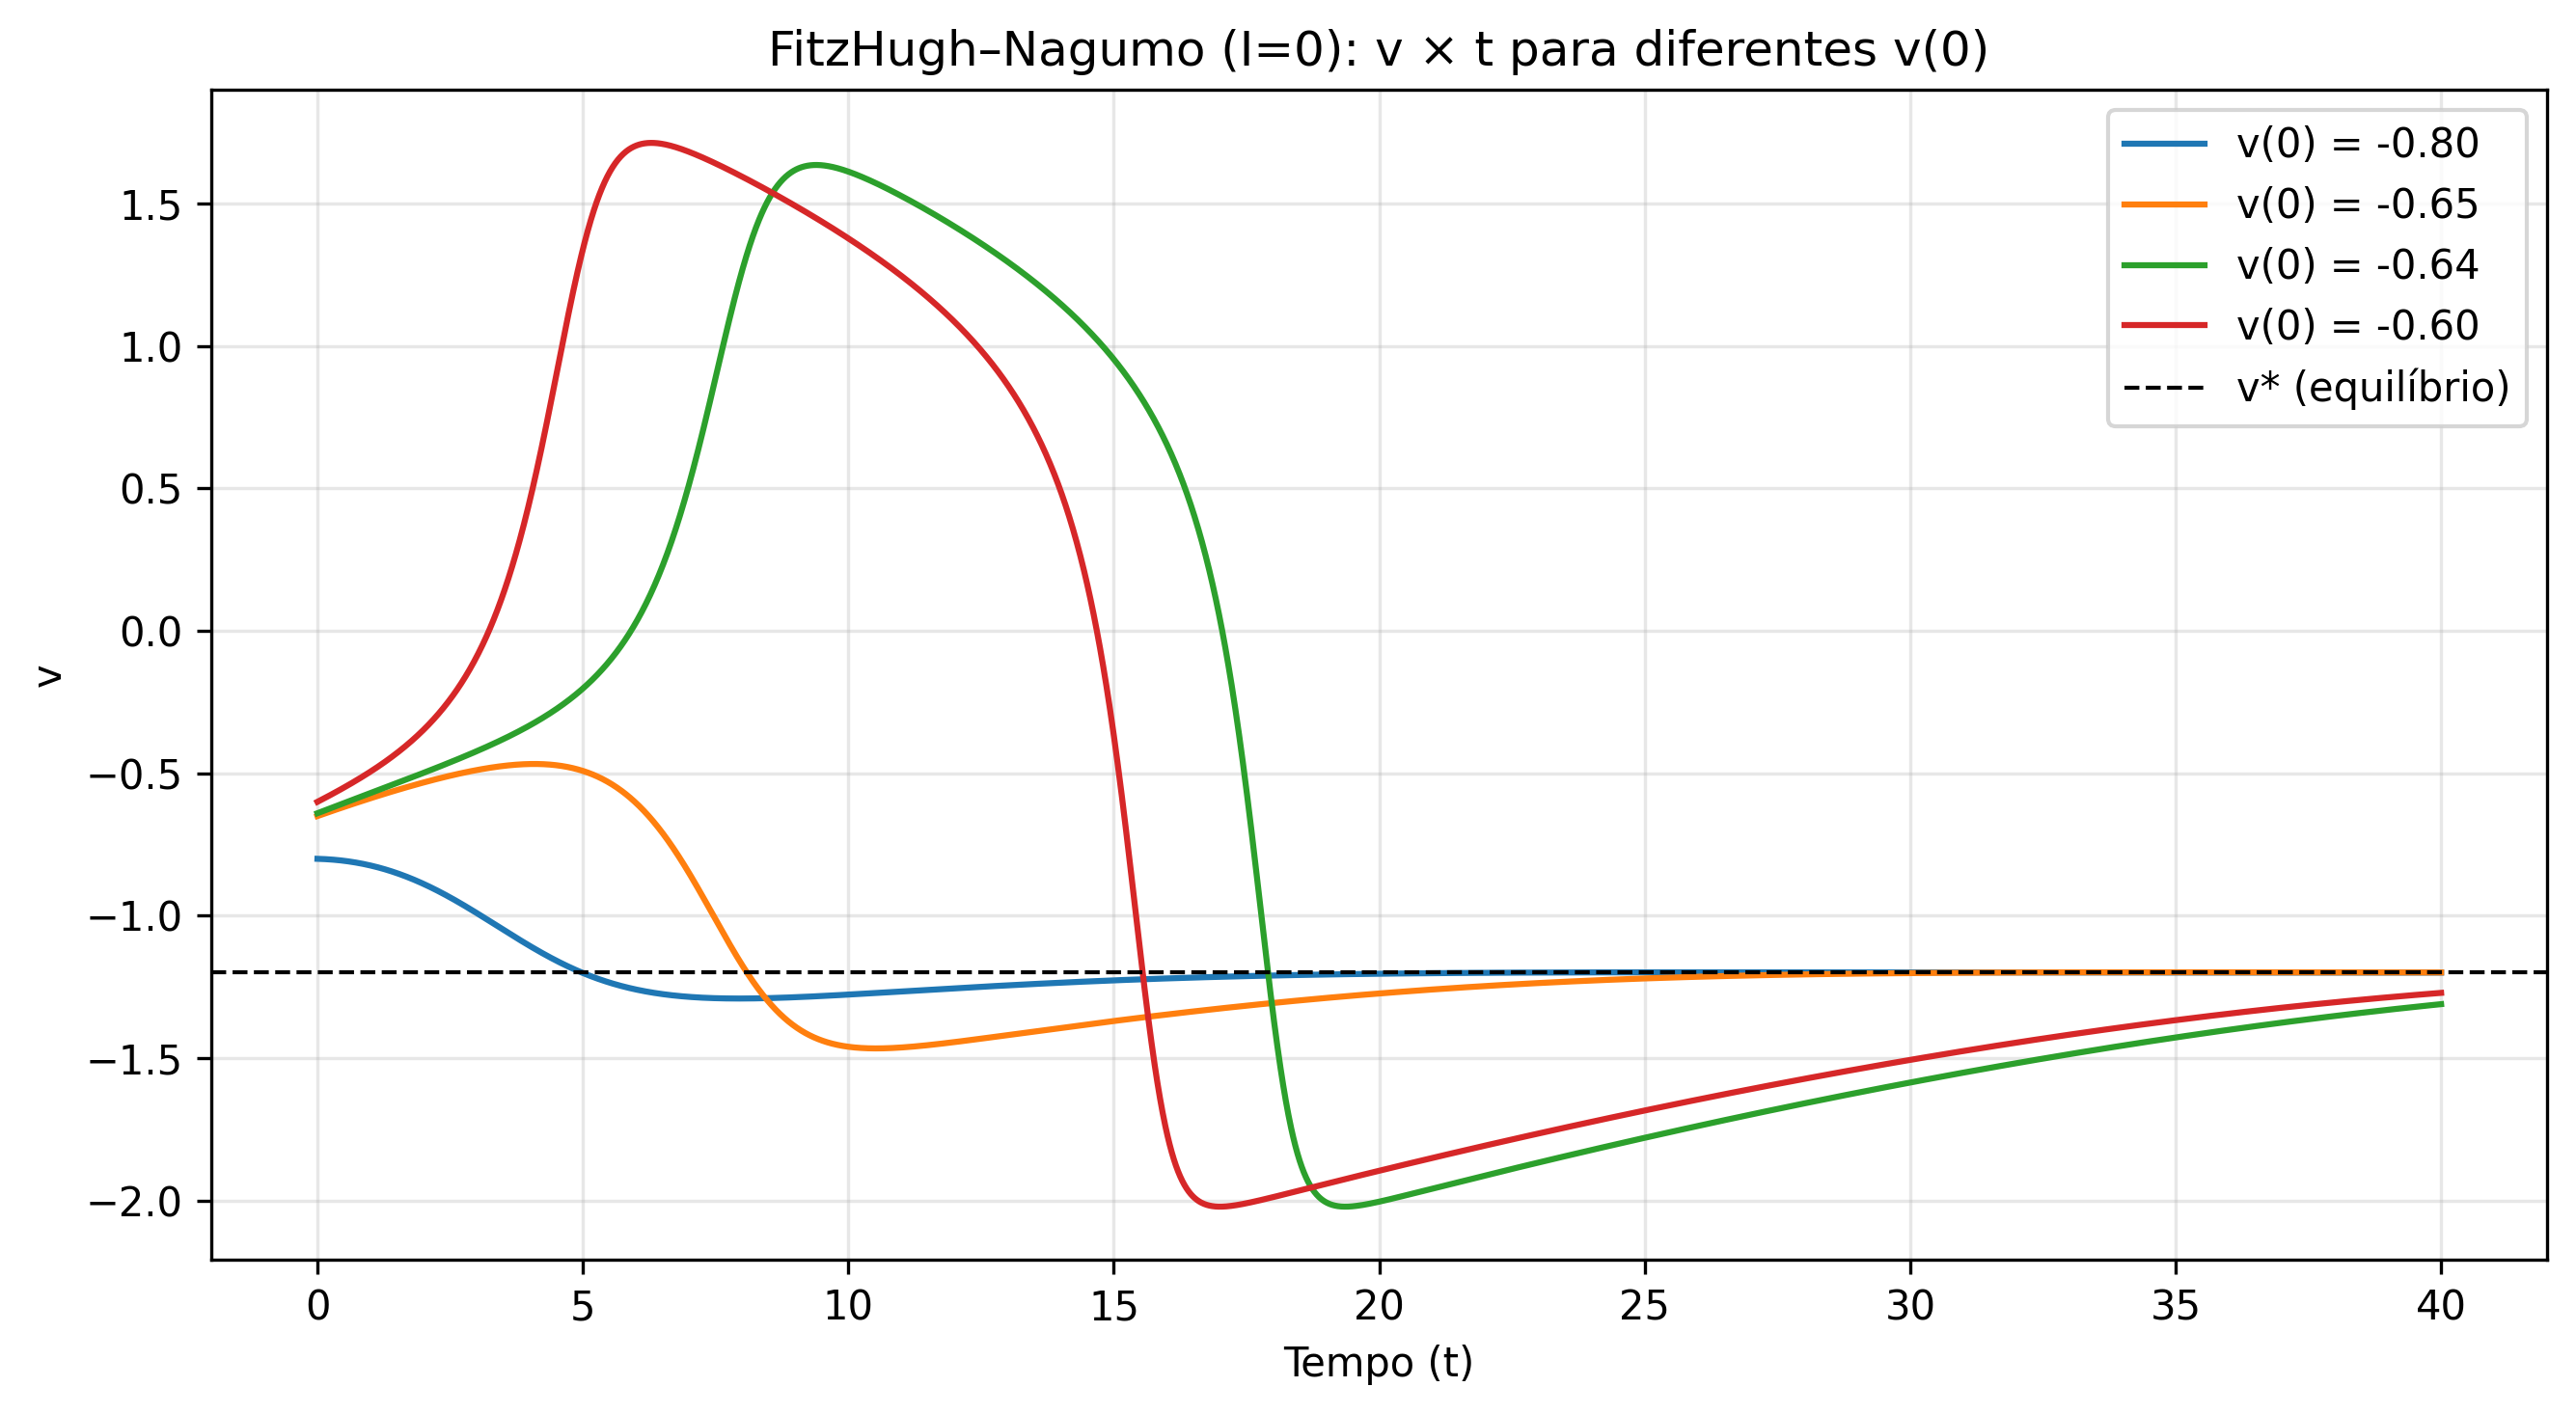
\includegraphics[width=11cm]{../figures/ex_1h_1.png}
		\caption{$v \times t$ do modelo FitzHugh-Nagumo para diferentes valores de $v(0)$.}
	\end{figure}
	
	\begin{figure}[H]
		\centering
		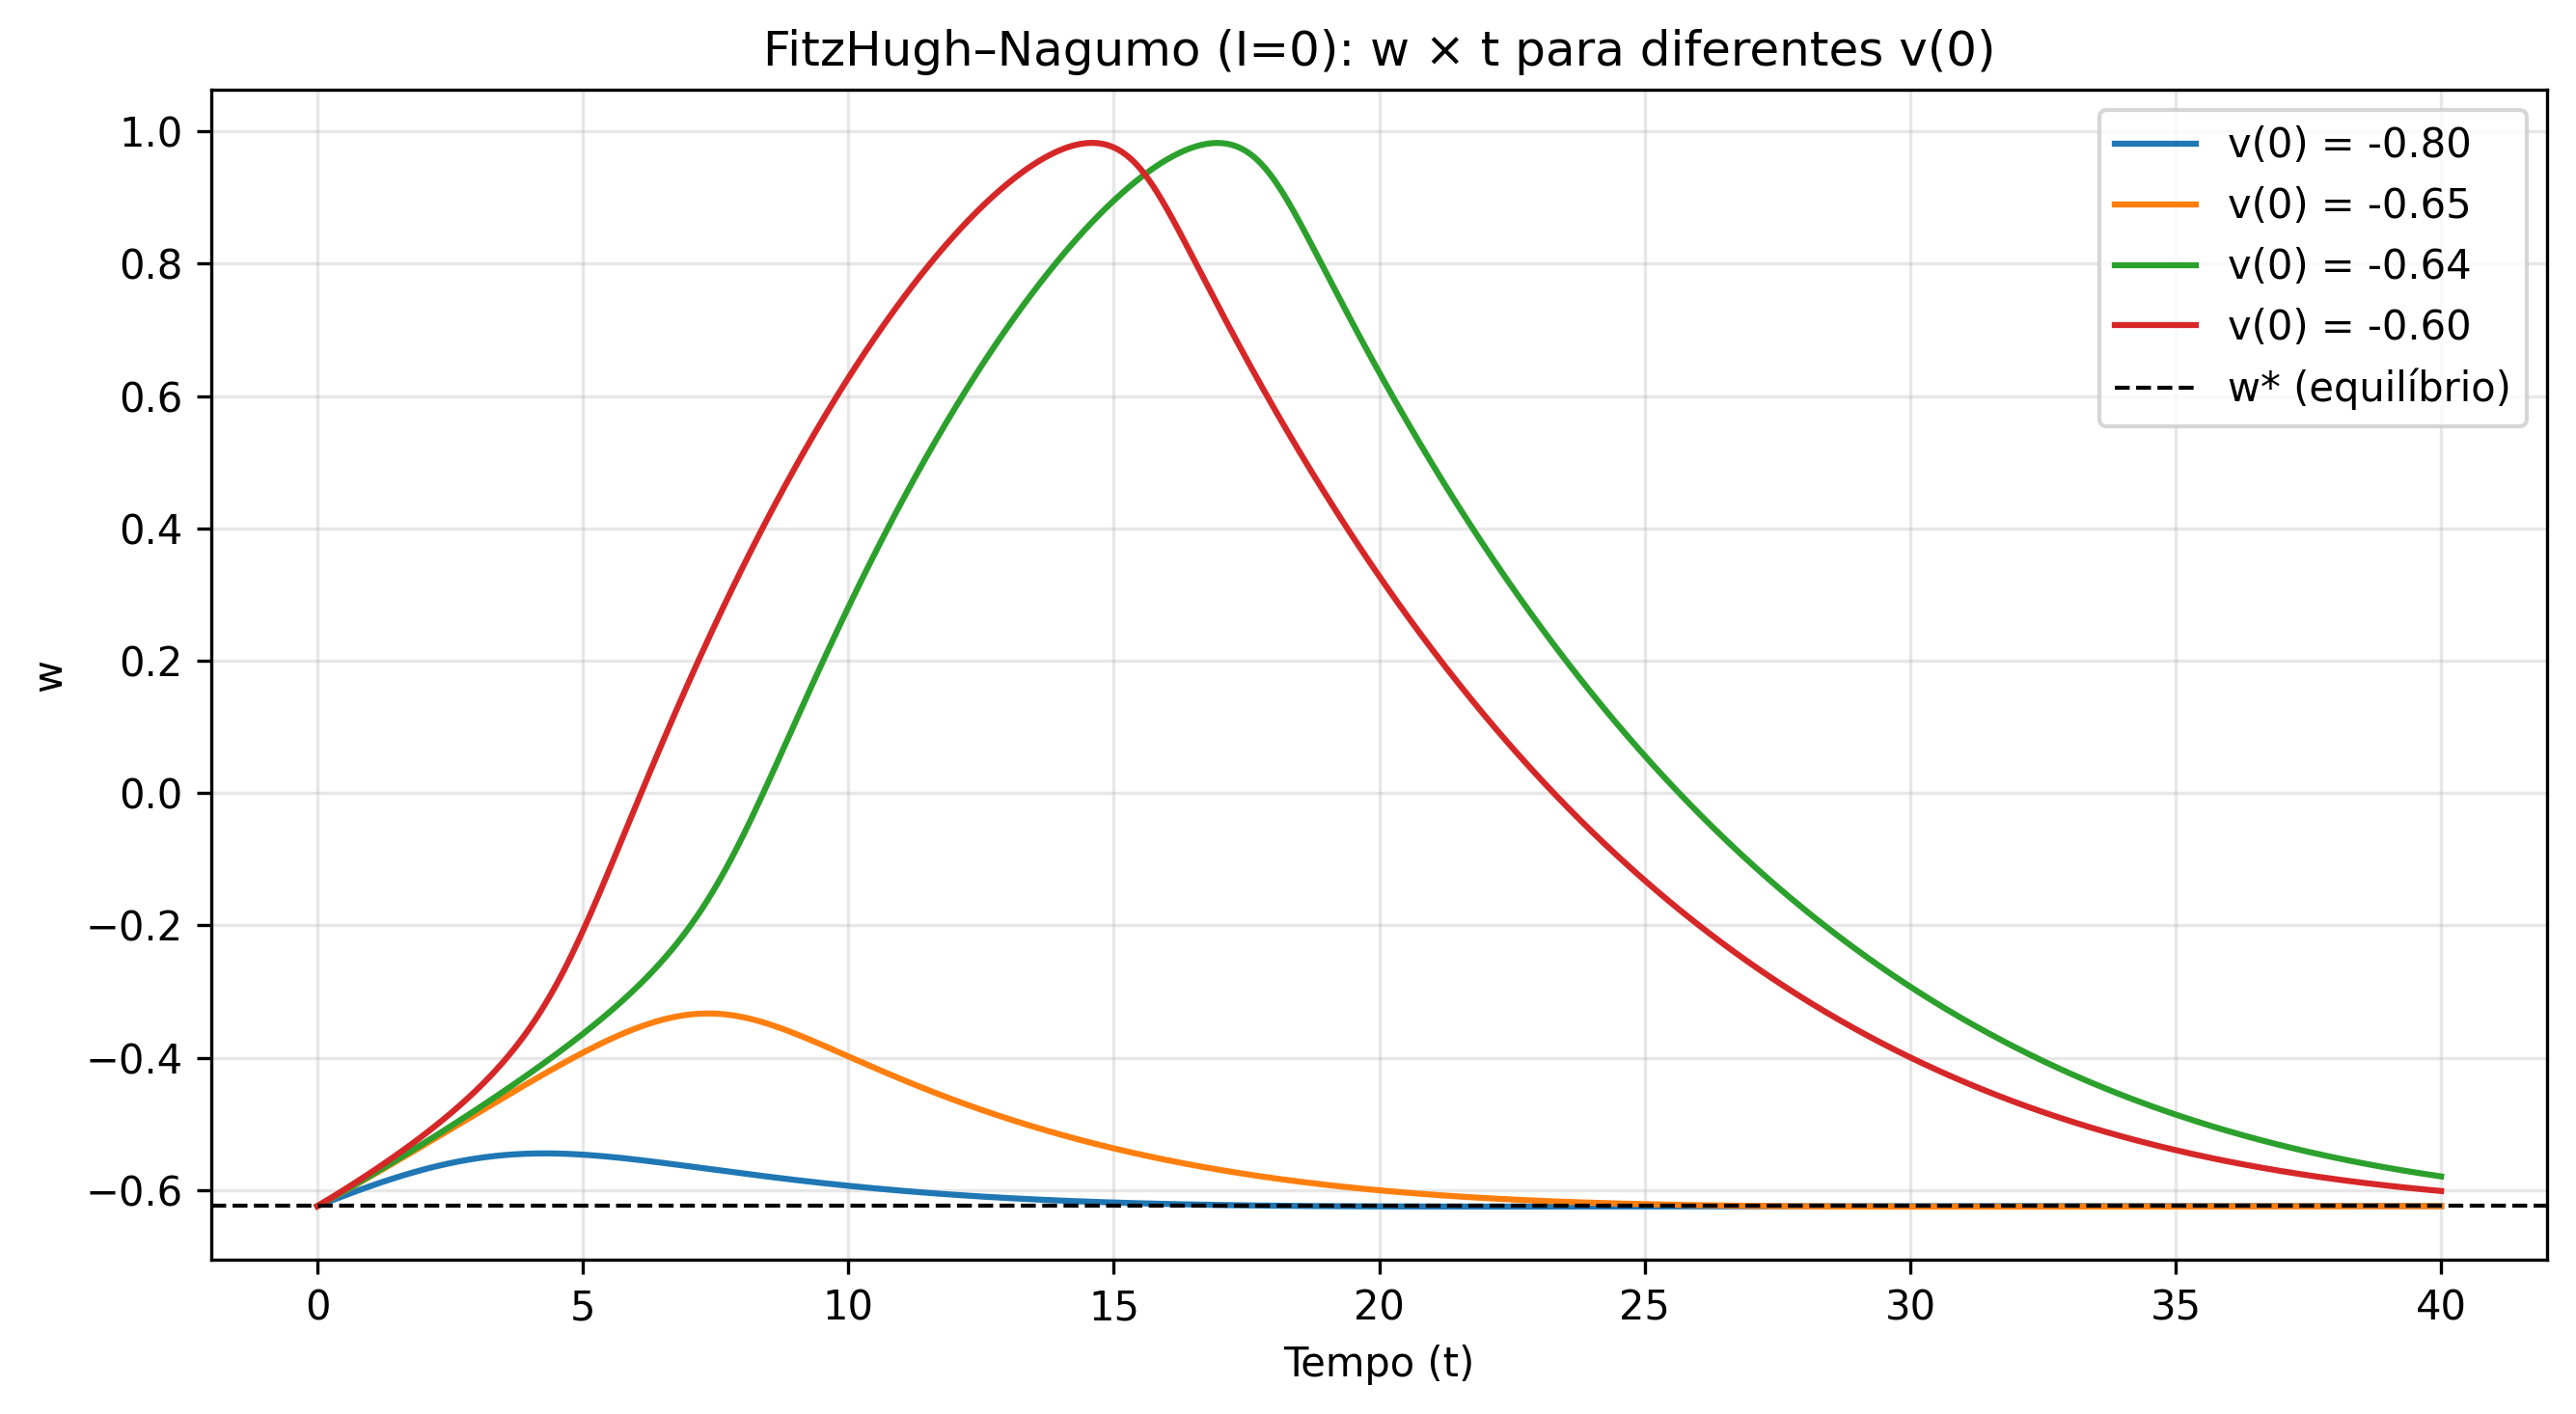
\includegraphics[width=11cm]{../figures/ex_1h_2.png}
		\caption{$w \times t$ do modelo FitzHugh-Nagumo para diferentes valores de $v(0)$}
	\end{figure}
	
	\begin{figure}[H]
		\centering
		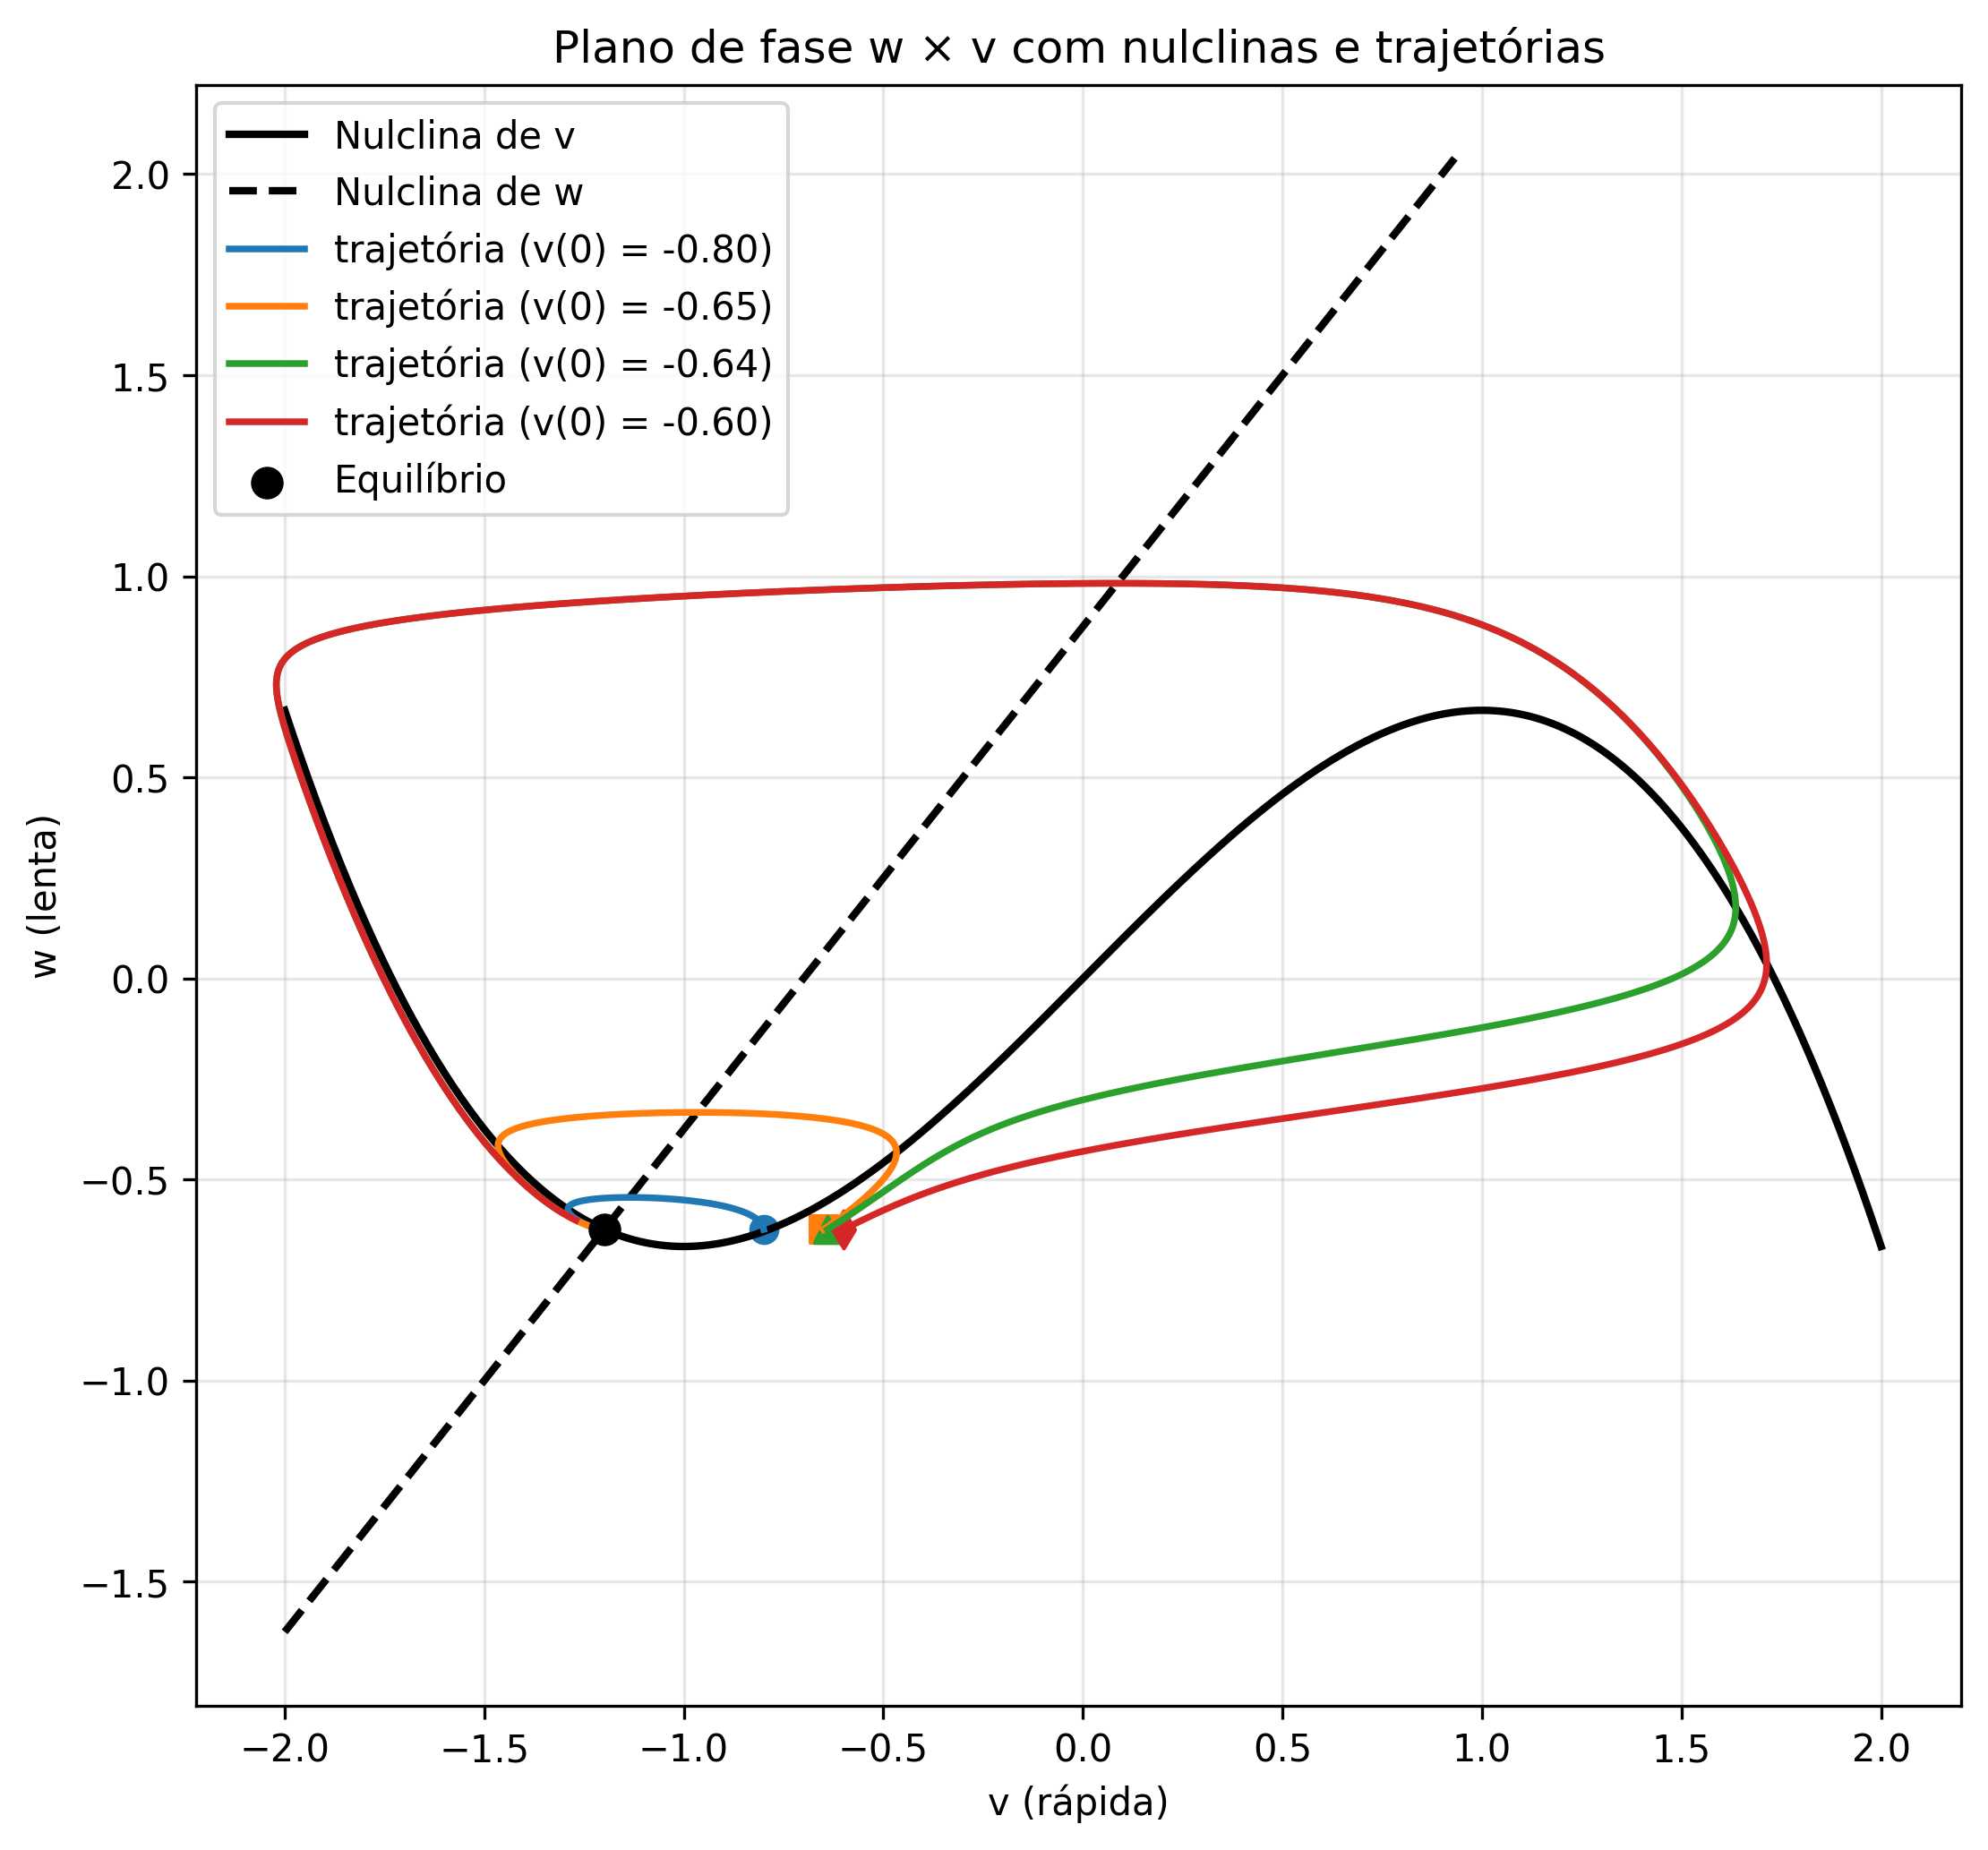
\includegraphics[width=11cm]{../figures/ex_1h_3.png}
		\caption{Plano de fase do modelo FitzHugh-Nagumo para diferentes valores de $v(0)$.}
	\end{figure}
	
	\noindent\textbf{(i)} Repita o que foi feito nos itens (a)-(g) para dois outros valores de $I$: $I = 1$ e $I = 1{,}5$.\\
	
	\noindent\textbf{Resposta:}
	
	\noindent\textit{Resultados resumidos para $I=1$ e $I=1{,}5$.}
	\[
	w_v(v)=v-\frac{v^3}{3}+I, 
	\qquad 
	w_w(v)=\frac{v+a}{b}, 
	\quad (a=0{,}7,\ b=0{,}8,\ \phi=0{,}08).
	\]
	No equilíbrio: \(w^{*}=w_v(v^{*})\). 
	Jacobiano em \((v^{*},w^{*})\): 
	\[
	J=\begin{bmatrix}p & q\\ r & s\end{bmatrix}
	=\begin{bmatrix}1-(v^{*})^2 & -1\\ \phi & -\phi b\end{bmatrix},\quad
	\tau=p+s,\ \Delta=ps-qr.
	\]
	
	\medskip
	\underline{\(\mathbf{I=1}\)}:
	\[
	\begin{aligned}
		&v^{*}\approx 0{,}408866,\qquad w^{*}\approx 1{,}386082,\\
		&p\approx 0{,}832829,\quad q=-1,\quad r=0{,}08,\quad s=-0{,}064,\\
		&\tau\approx 0{,}768829,\quad \Delta\approx 0{,}026699,\\
		&\lambda_{1,2}\approx 0{,}732373\ \ \text{e}\ \ 0{,}036455\quad(\text{reais e positivos}).
	\end{aligned}
	\]
	\(\Rightarrow\) \textbf{nó instável} (hiperbólico).
	
	\medskip
	\underline{\(\mathbf{I=1{,}5}\)}:
	\[
	\begin{aligned}
		&v^{*}\approx 1{,}032480,\qquad w^{*}\approx 2{,}165600,\\
		&p\approx -0{,}066015,\quad q=-1,\quad r=0{,}08,\quad s=-0{,}064,\\
		&\tau\approx -0{,}130015,\quad \Delta\approx 0{,}084225,\\
		&\lambda_{1,2}\approx -0{,}065008 \pm 0{,}282841\,i\quad(\text{complexos, parte real negativa}).
	\end{aligned}
	\]
	\(\Rightarrow\) \textbf{foco estável} (hiperbólico).\\\\
	
	
	\noindent\textbf{(j)} Use o seu programa para simular as equações do modelo de FitzHugh-Nagumo para simular o modelo nos casos em que $I = 1$ e $I = 1{,}5$. Use como condição inicial para os dois casos o ponto de equilíbrio do sistema para $I = 0$. Nestes casos, faça o programa gerar, para cada valor de $I$, os gráficos de $v \times t$ e $w \times t$ e o plano de fase $w \times v$ mostrando as nulclinas de $v$ e $w$ e as trajetórias correspondentes. Interprete seus resultados à luz do que foi discutido na aula de análise qualitativa do modelo de Hodgkin-Huxley usando os resultados obtidos no item (i) acima. Pode ser útil também ler o artigo sobre o modelo de FitzHugh-Nagumo na Scholarpedia (\url{http://www.scholarpedia.org/article/FitzHugh-Nagumo_model}), especificamente o tópico sobre bloqueio por excitação (\textit{excitation block} em inglês).\\
	
	\noindent\textbf{Resposta:}
	
	\begin{figure}[H]
		\centering
		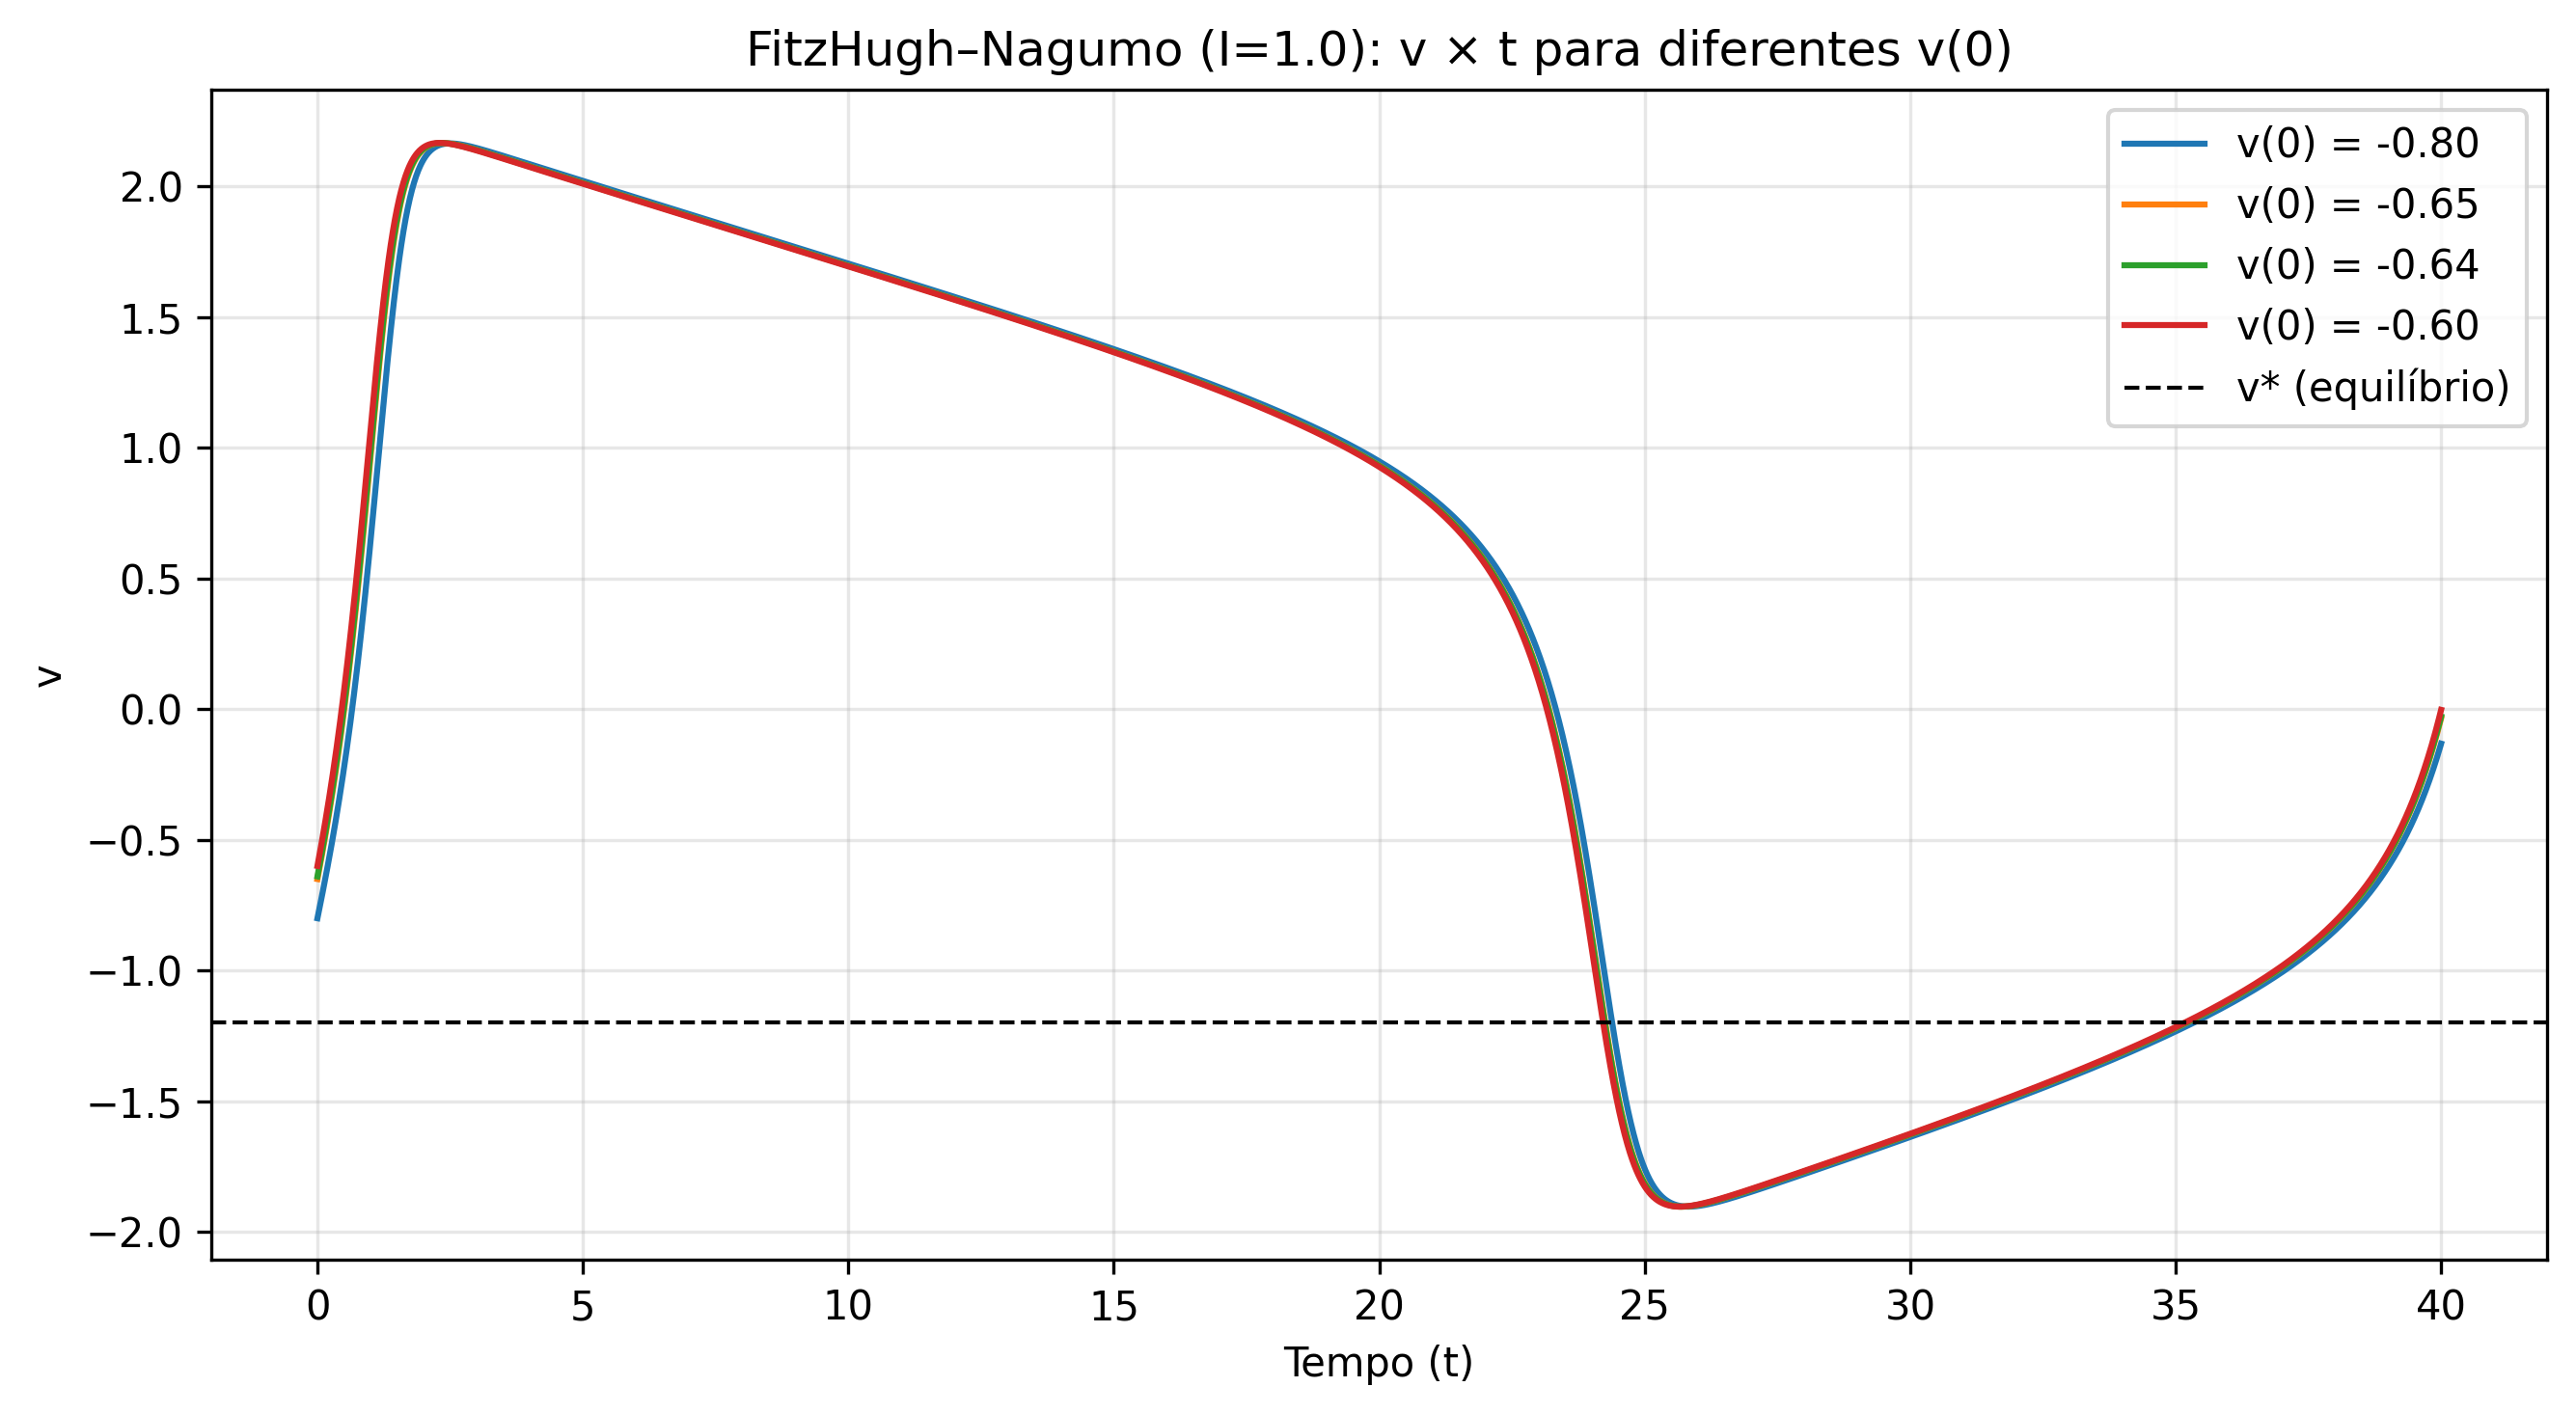
\includegraphics[width=11cm]{../figures/ex_1j_I1.0_1.png}
		\caption{$v \times t$ do modelo FitzHugh-Nagumo para diferentes valores de $v(0)$ e $I = 1.0$.}
	\end{figure}
	
	\begin{figure}[H]
		\centering
		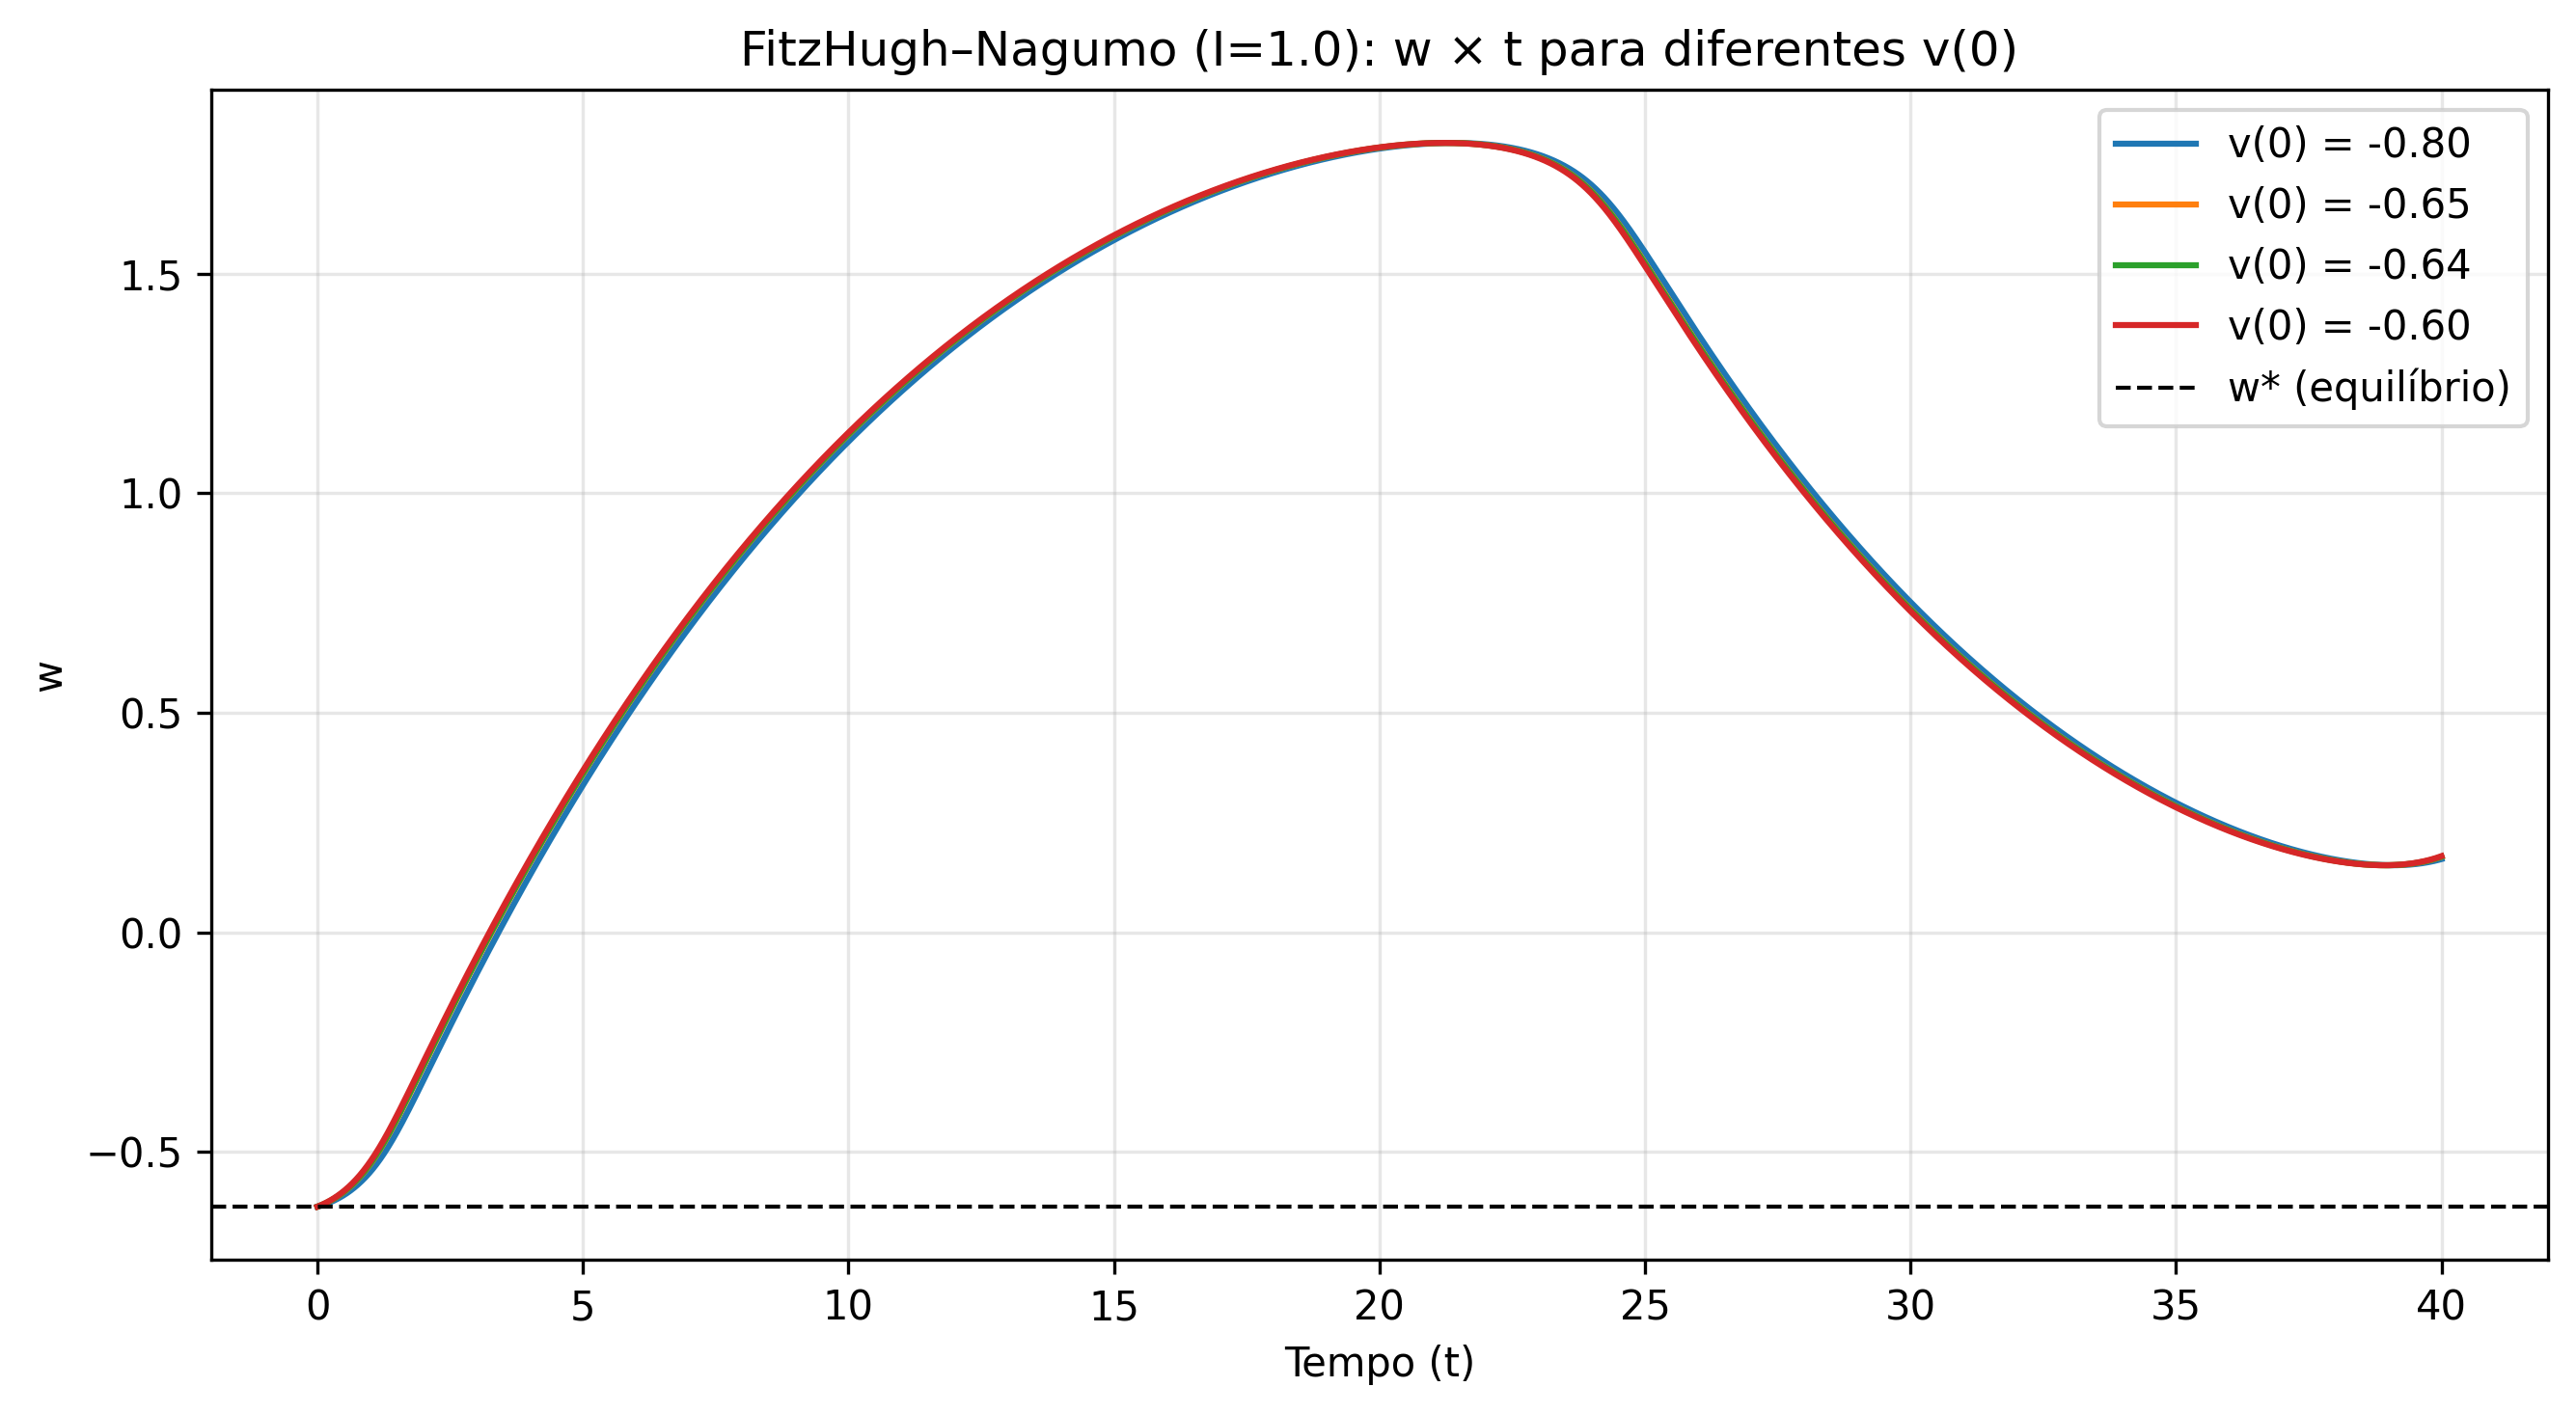
\includegraphics[width=11cm]{../figures/ex_1j_I1.0_2.png}
		\caption{$w \times t$ do modelo FitzHugh-Nagumo para diferentes valores de $v(0)$ e $I = 1.0$.}
	\end{figure}
	
	\begin{figure}[H]
		\centering
		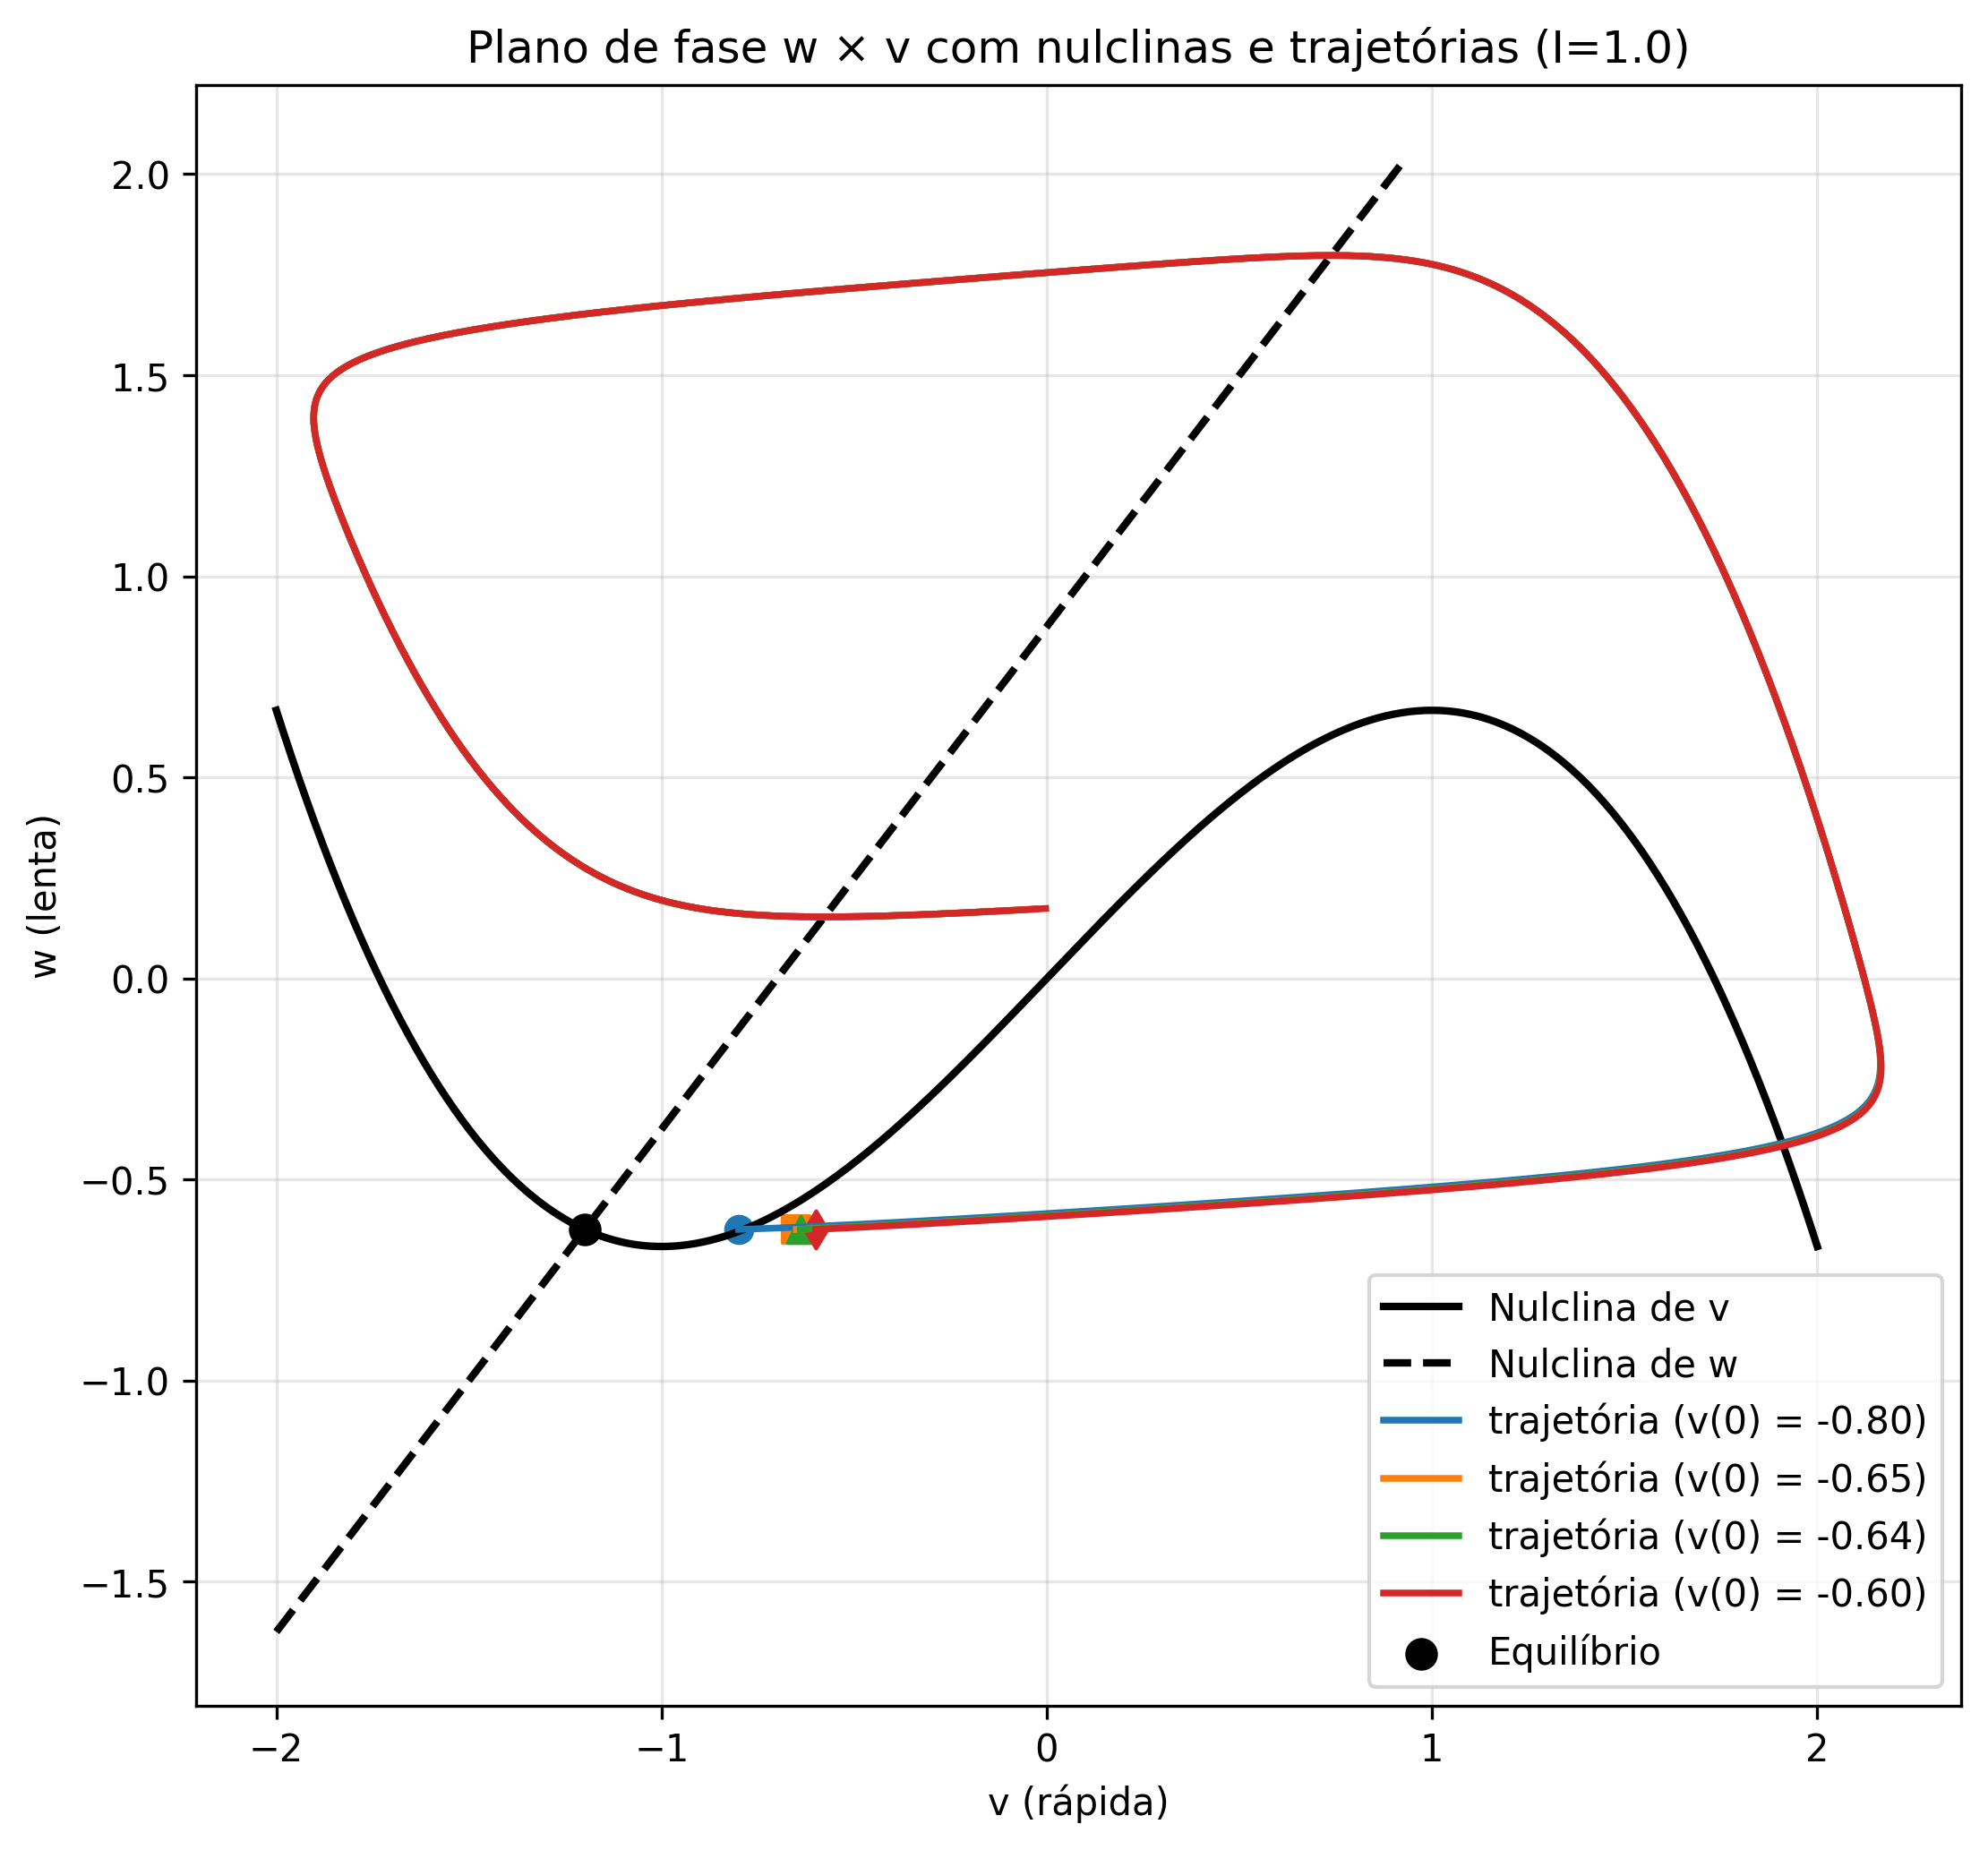
\includegraphics[width=11cm]{../figures/ex_1j_I1.0_3.png}
		\caption{Plano de fase do modelo FitzHugh-Nagumo para diferentes valores de $v(0)$ e $I = 1.0$.}
	\end{figure}
	
	\begin{figure}[H]
		\centering
		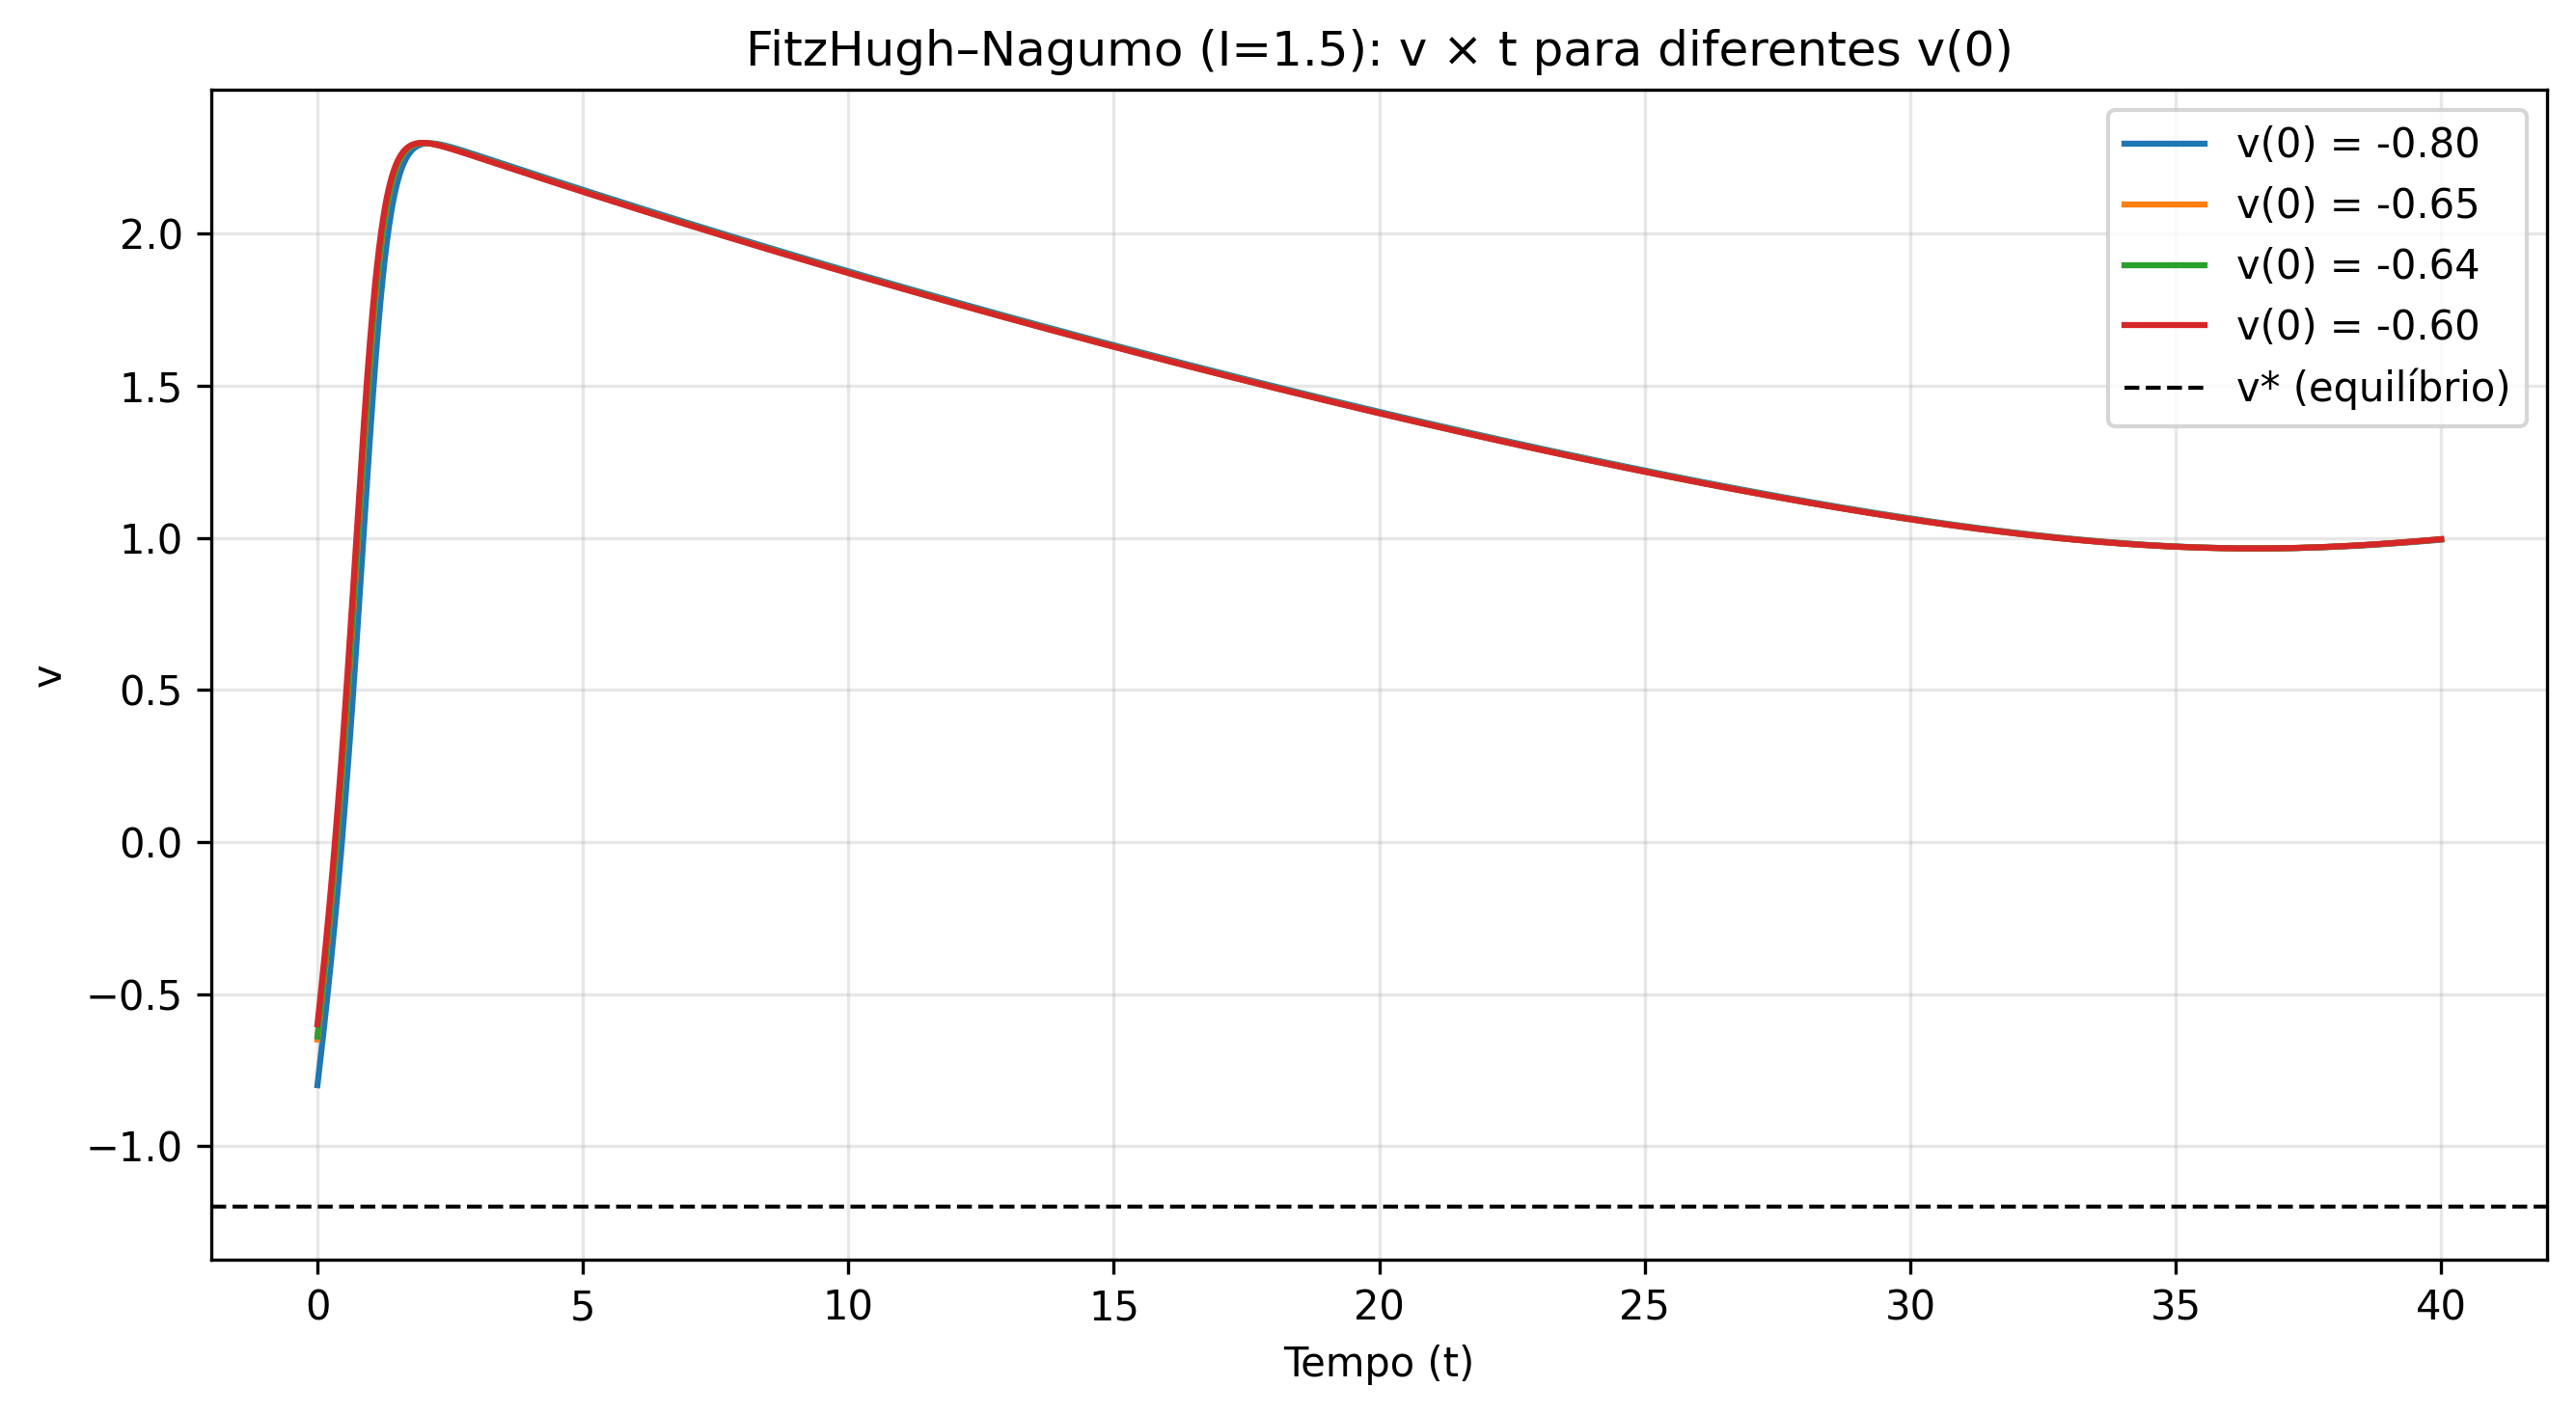
\includegraphics[width=11cm]{../figures/ex_1j_I1.5_1.png}
		\caption{$v \times t$ do modelo FitzHugh-Nagumo para diferentes valores de $v(0)$ e $I = 1.5$.}
	\end{figure}
	
	\begin{figure}[H]
		\centering
		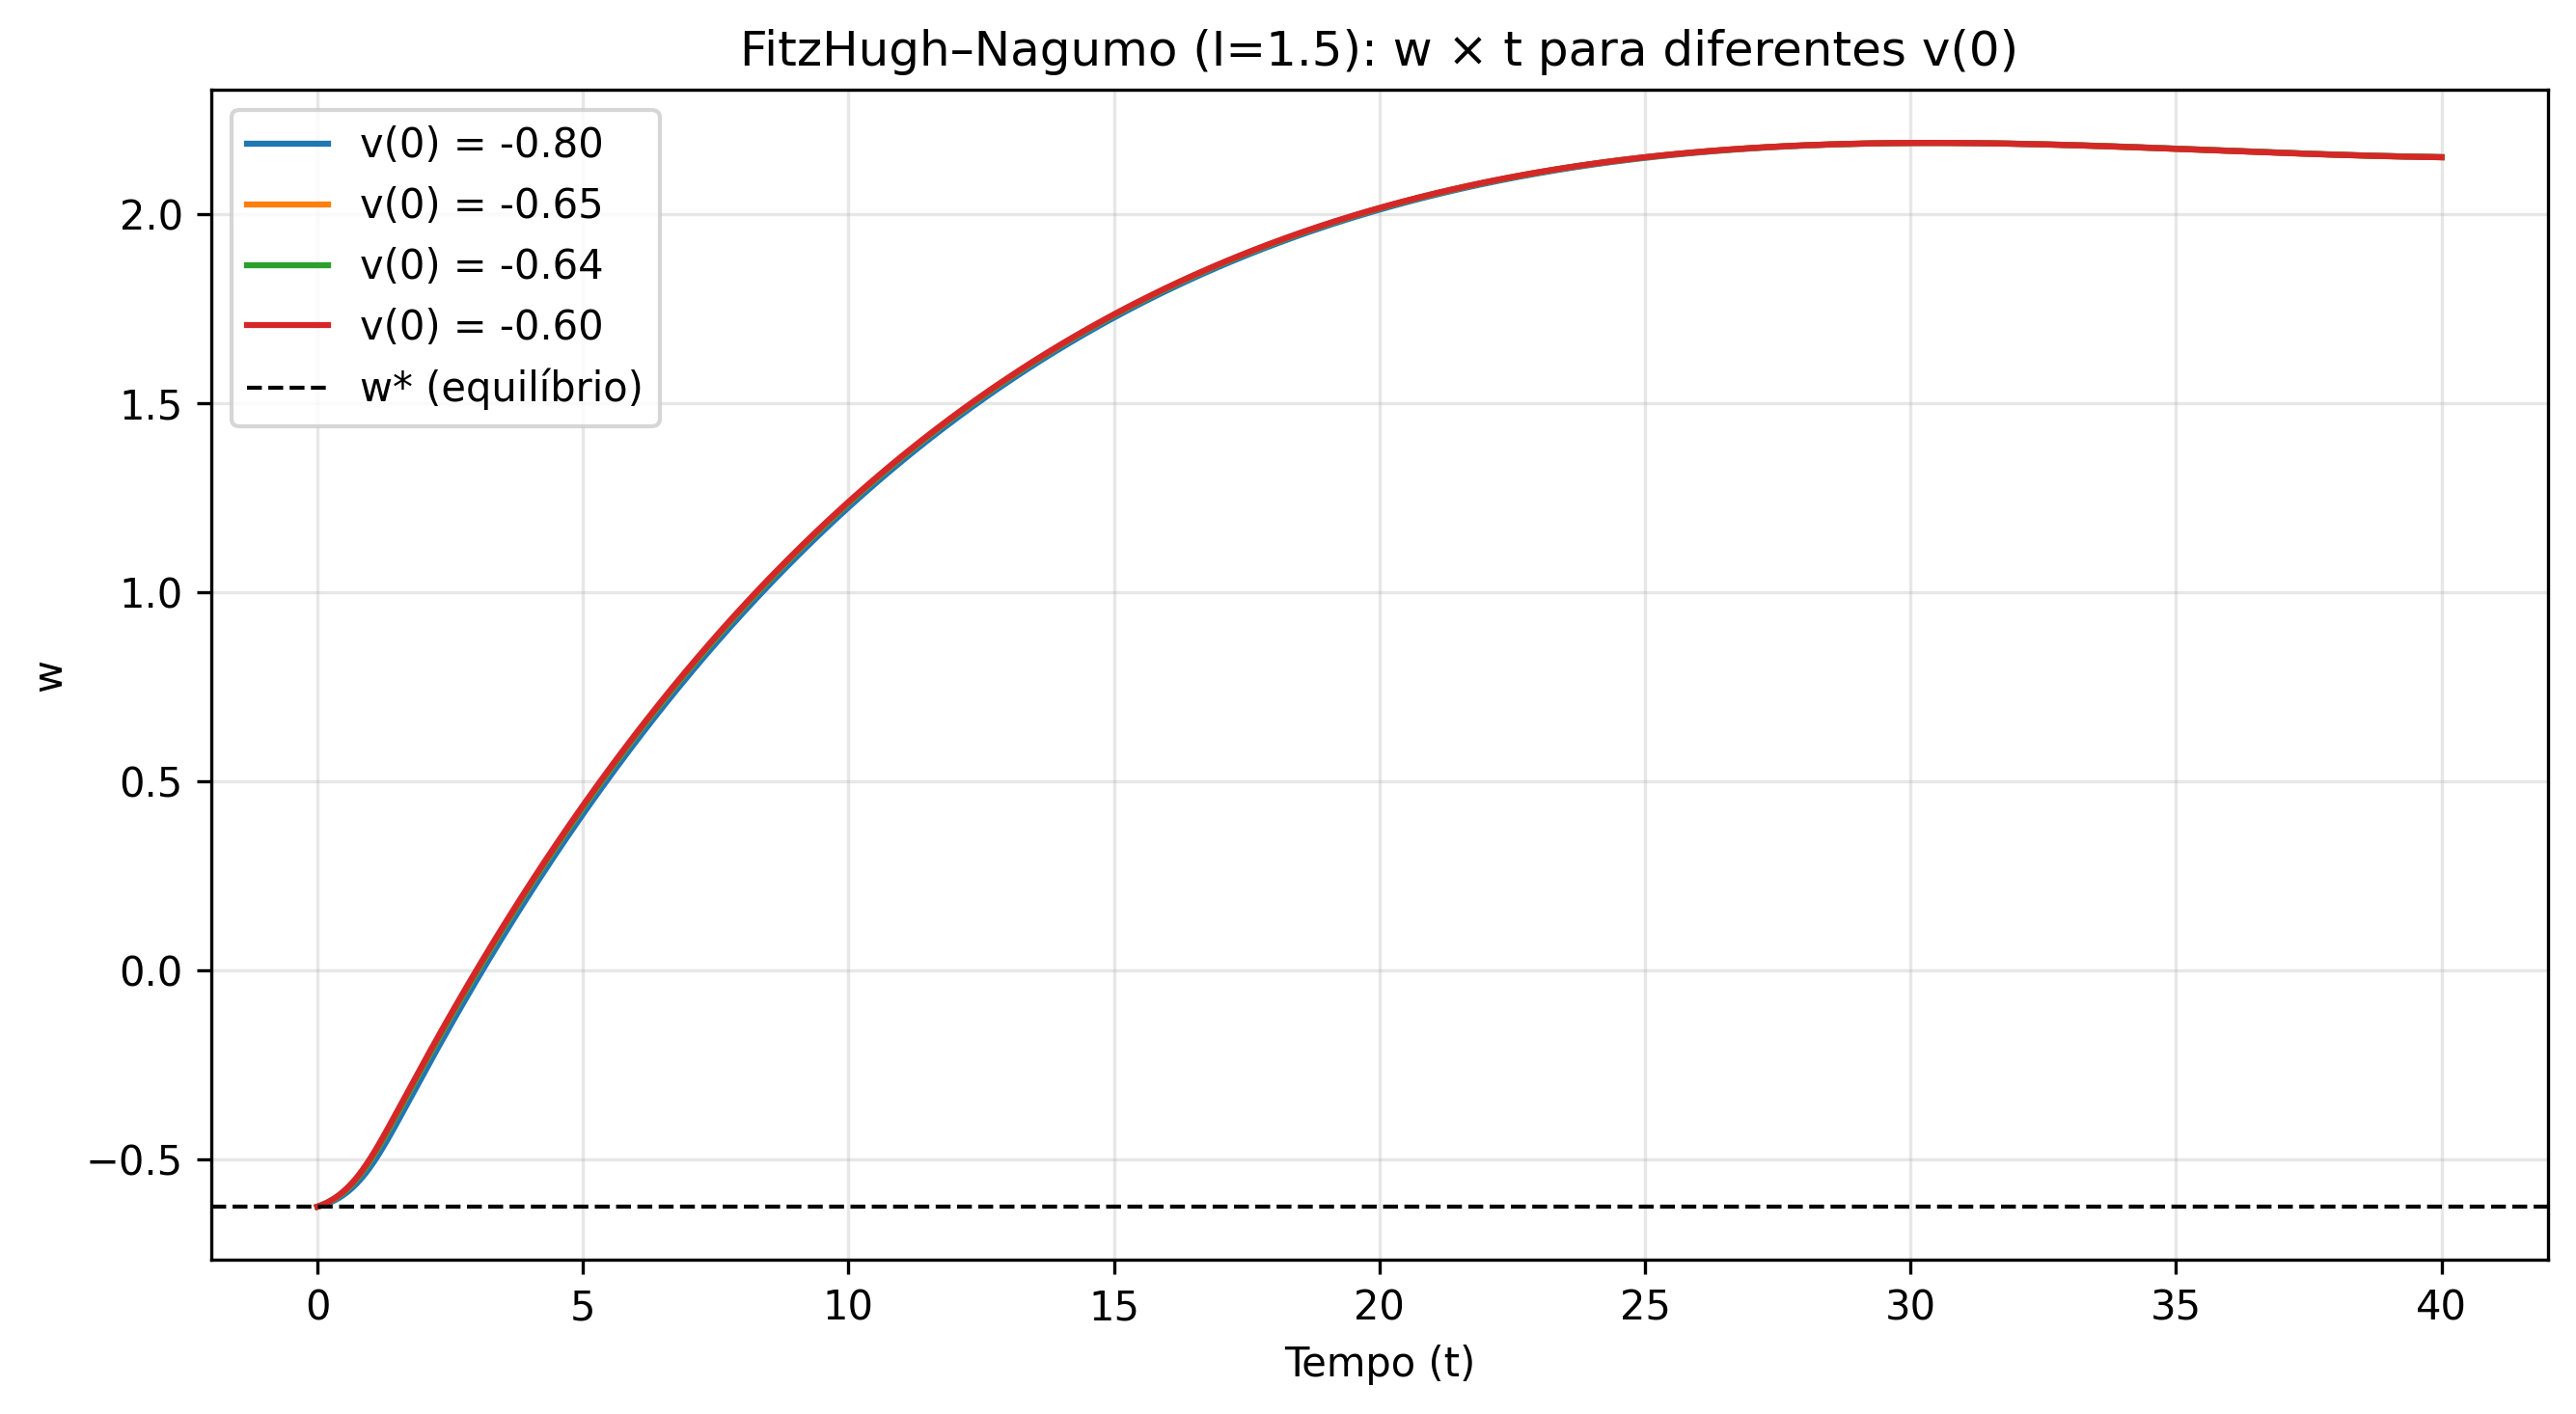
\includegraphics[width=11cm]{../figures/ex_1j_I1.5_2.png}
		\caption{$w \times t$ do modelo FitzHugh-Nagumo para diferentes valores de $v(0)$ e $I = 1.5$.}
	\end{figure}
	
	\begin{figure}[H]
		\centering
		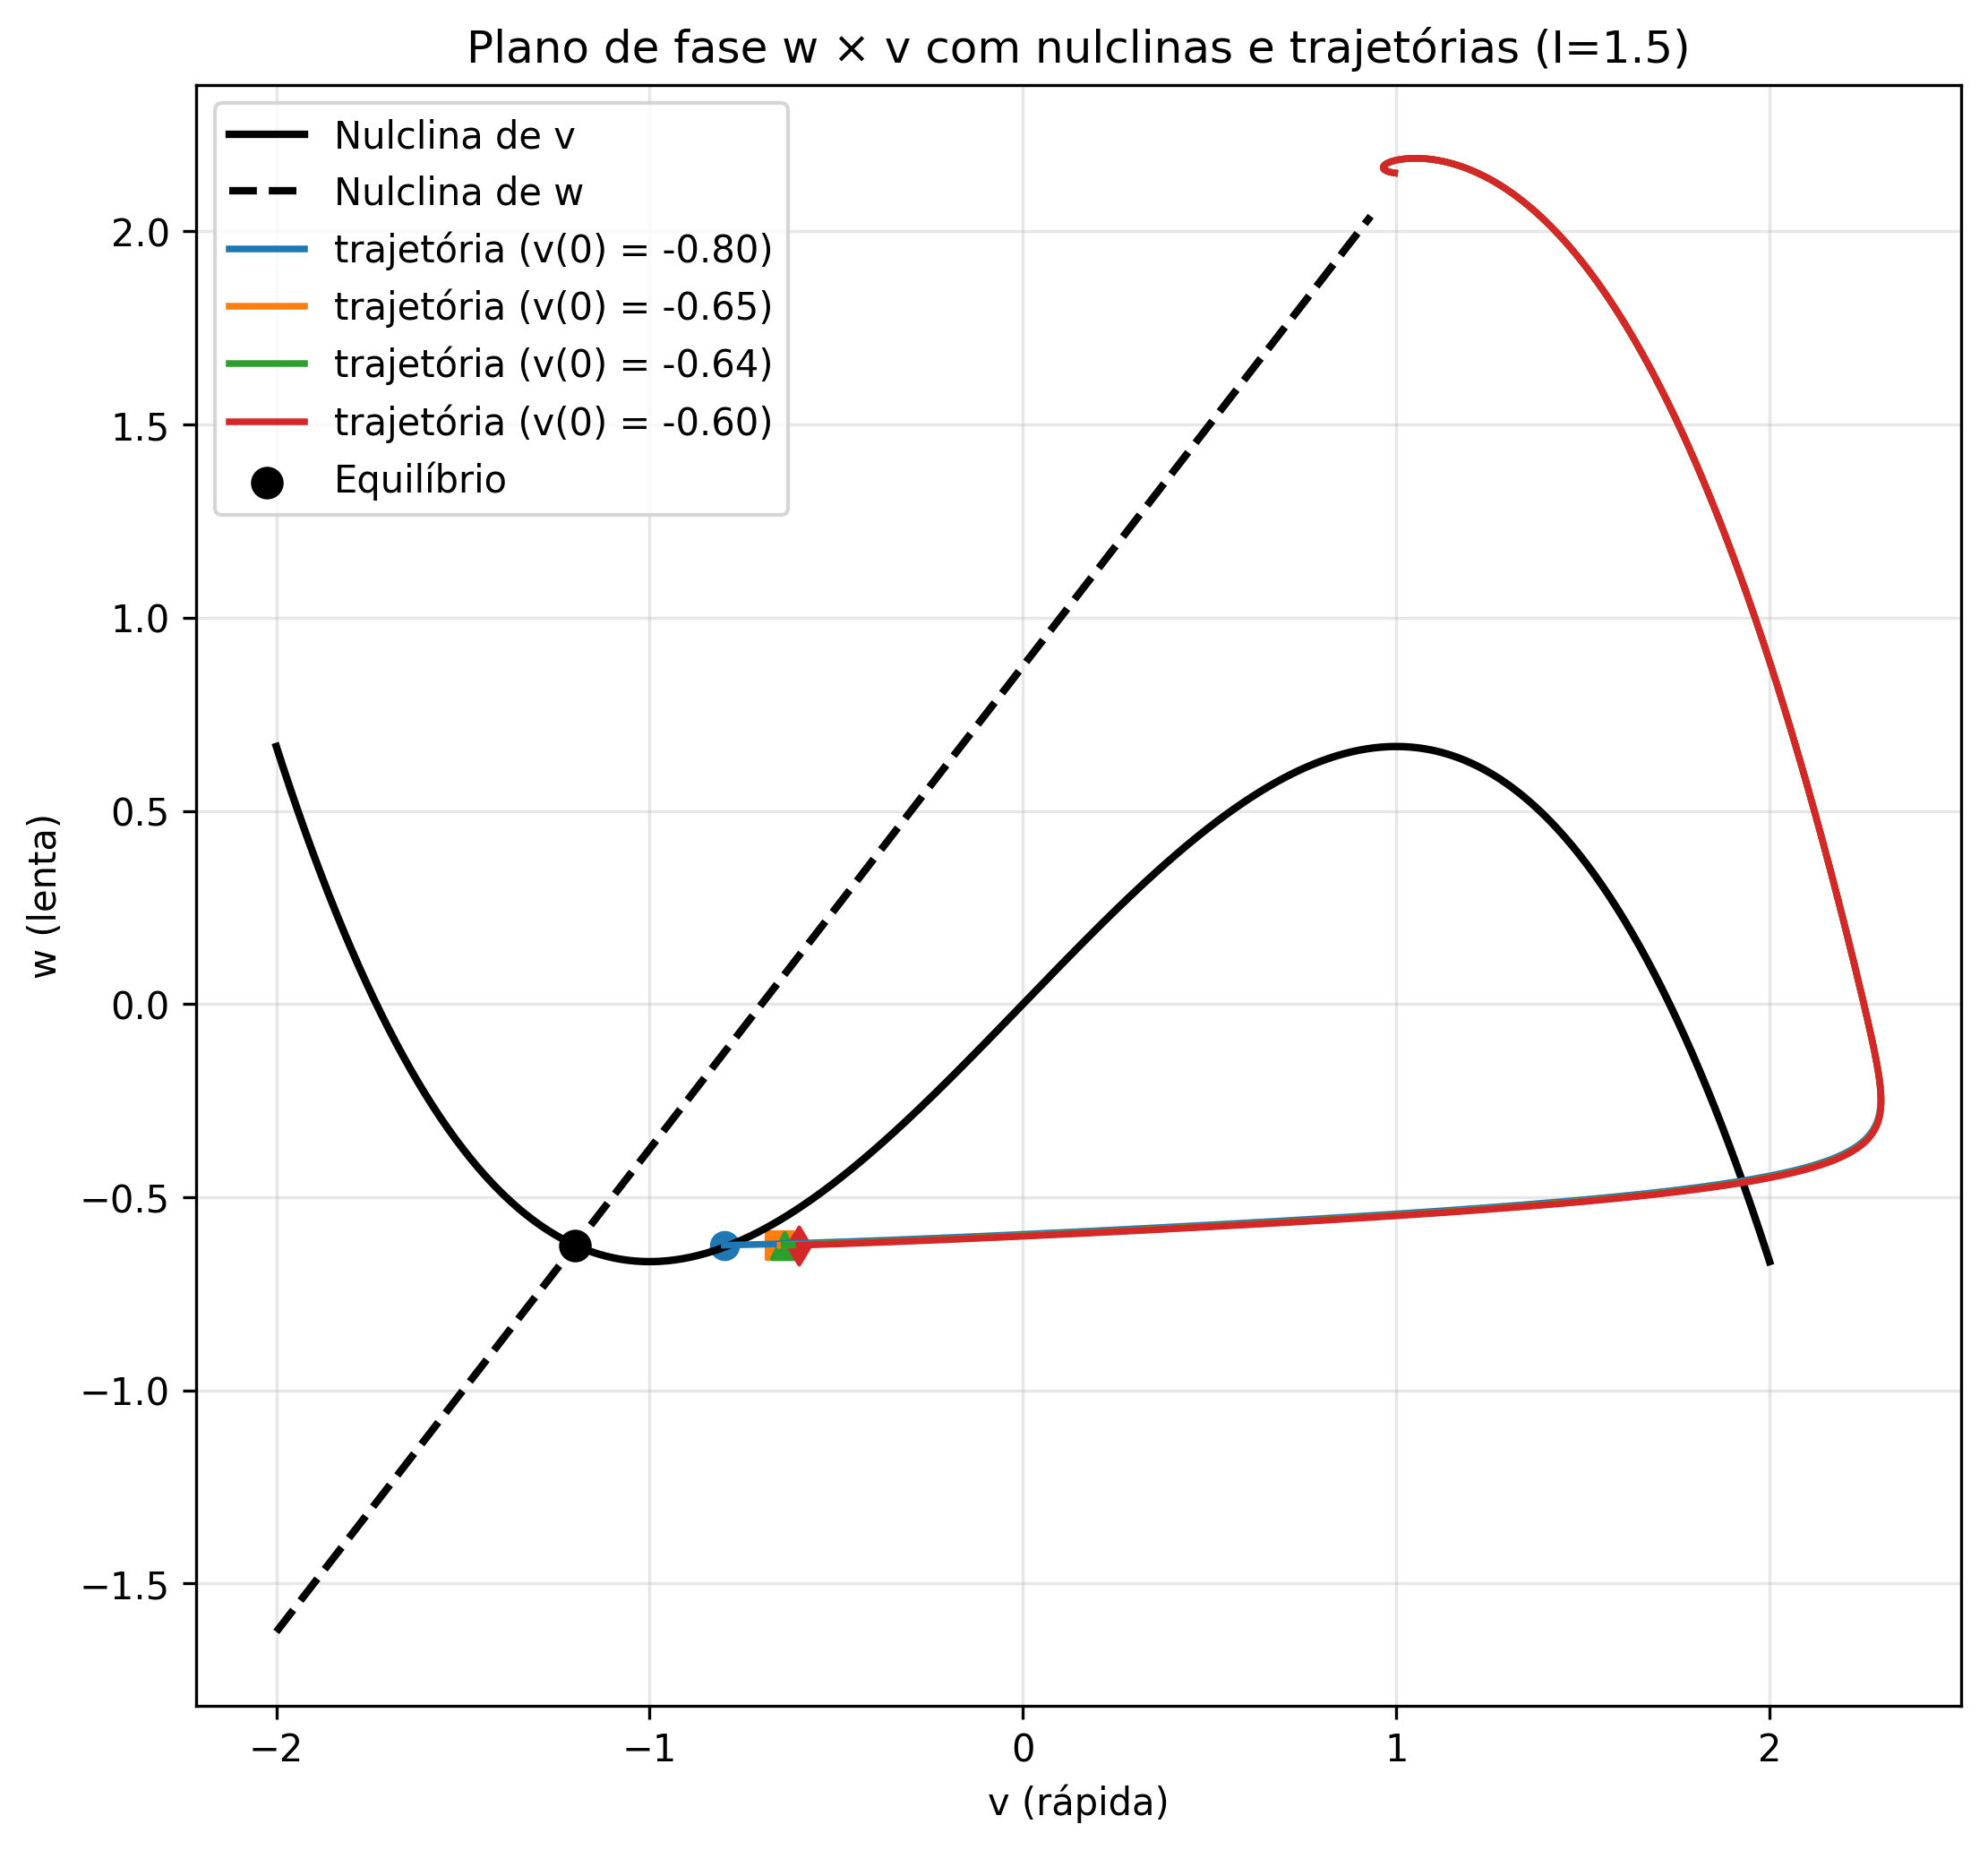
\includegraphics[width=11cm]{../figures/ex_1j_I1.5_3.png}
		\caption{Plano de fase do modelo FitzHugh-Nagumo para diferentes valores de $v(0)$ e $I = 1.5$.}
	\end{figure}
	
	\noindent\textbf{Interpretação dos gráficos — casos $I=1$ e $I=1{,}5$.}
	
	\medskip
	\underline{\textbf{$I=1$ (oscilatório)}}.
	Partindo do equilíbrio de $I=0$, o degrau em $I$ desloca a nulclina cúbica para cima e o equilíbrio para o ramo médio, que é instável (nó instável; cf. item (i)). 
	Nos gráficos $v\times t$ e $w\times t$ observa-se um \emph{pico de despolarização} rápido (dinâmica da variável rápida $v$), seguido de uma fase de \emph{plateau} com variação lenta (controle por $w$) e, por fim, uma \emph{repolarização} rápida; o ciclo reinicia, indicando \textbf{oscilação sustentada} (limite cíclico). 
	No plano de fase $w\times v$, a trajetória contorna a cúbica: (i) subida rápida para o ramo direito; (ii) deriva lenta ao longo do ramo direito conforme $w$ cresce; (iii) salto pelo ramo instável; (iv) deriva lenta pelo ramo esquerdo. 
	As diferentes condições iniciais de $v(0)$ convergem para a \textbf{mesma órbita} (atração para o limite cíclico), coerente com o fato de o equilíbrio local ser instável.
	
	\medskip
	\underline{\textbf{$I=1{,}5$ (bloqueio por excitação / estado despolarizado)}}.
	Com $I$ maior, o equilíbrio se desloca para o ramo direito e torna-se \textbf{estável} (foco estável; cf. item (i)).
	Nos gráficos $v\times t$ e $w\times t$, após um overshoot inicial, $v(t)$ e $w(t)$ aproximam-se \emph{monotônica} (ou quase-) e \emph{lentamente} de $(v^*,w^*)$ no patamar alto (depolarizado), sem oscilações sustentadas. 
	No plano de fase, todas as trajetórias entram na bacia de atração do ponto fixo no ramo direito e convergem a ele.
	Esse regime corresponde ao \textbf{bloqueio por excitação}: correntes tônicas grandes suprimem o ciclo-limite e o neurônio permanece em um estado despolarizado estável, como discutido qualitativamente para Hodgkin--Huxley e no verbete do FitzHugh--Nagumo (``\textit{excitation block}'').
	
	\medskip
	\noindent\textbf{Síntese.} 
	A transição entre os dois regimes é compatível com a análise no plano $(\tau,\Delta)$: para $I=1$ o equilíbrio está na região \emph{instável} (o que sugere a existência de um limite cíclico atrator), enquanto para $I=1{,}5$ cruza-se a fronteira (próximo de uma bifurcação de Andronov--Hopf), e o equilíbrio passa a \emph{estável}, eliminando as oscilações sustentadas.\\\\
	
	
	\noindent\textbf{(k)} Construa a curva f-I do modelo de FitzHugh-Nagumo para $I$ no intervalo $0 \leq I \leq 1$. O modelo é de tipo I ou tipo II?\\
	
	\noindent\textbf{Resposta:}
	
	\begin{figure}[H]
		\centering
		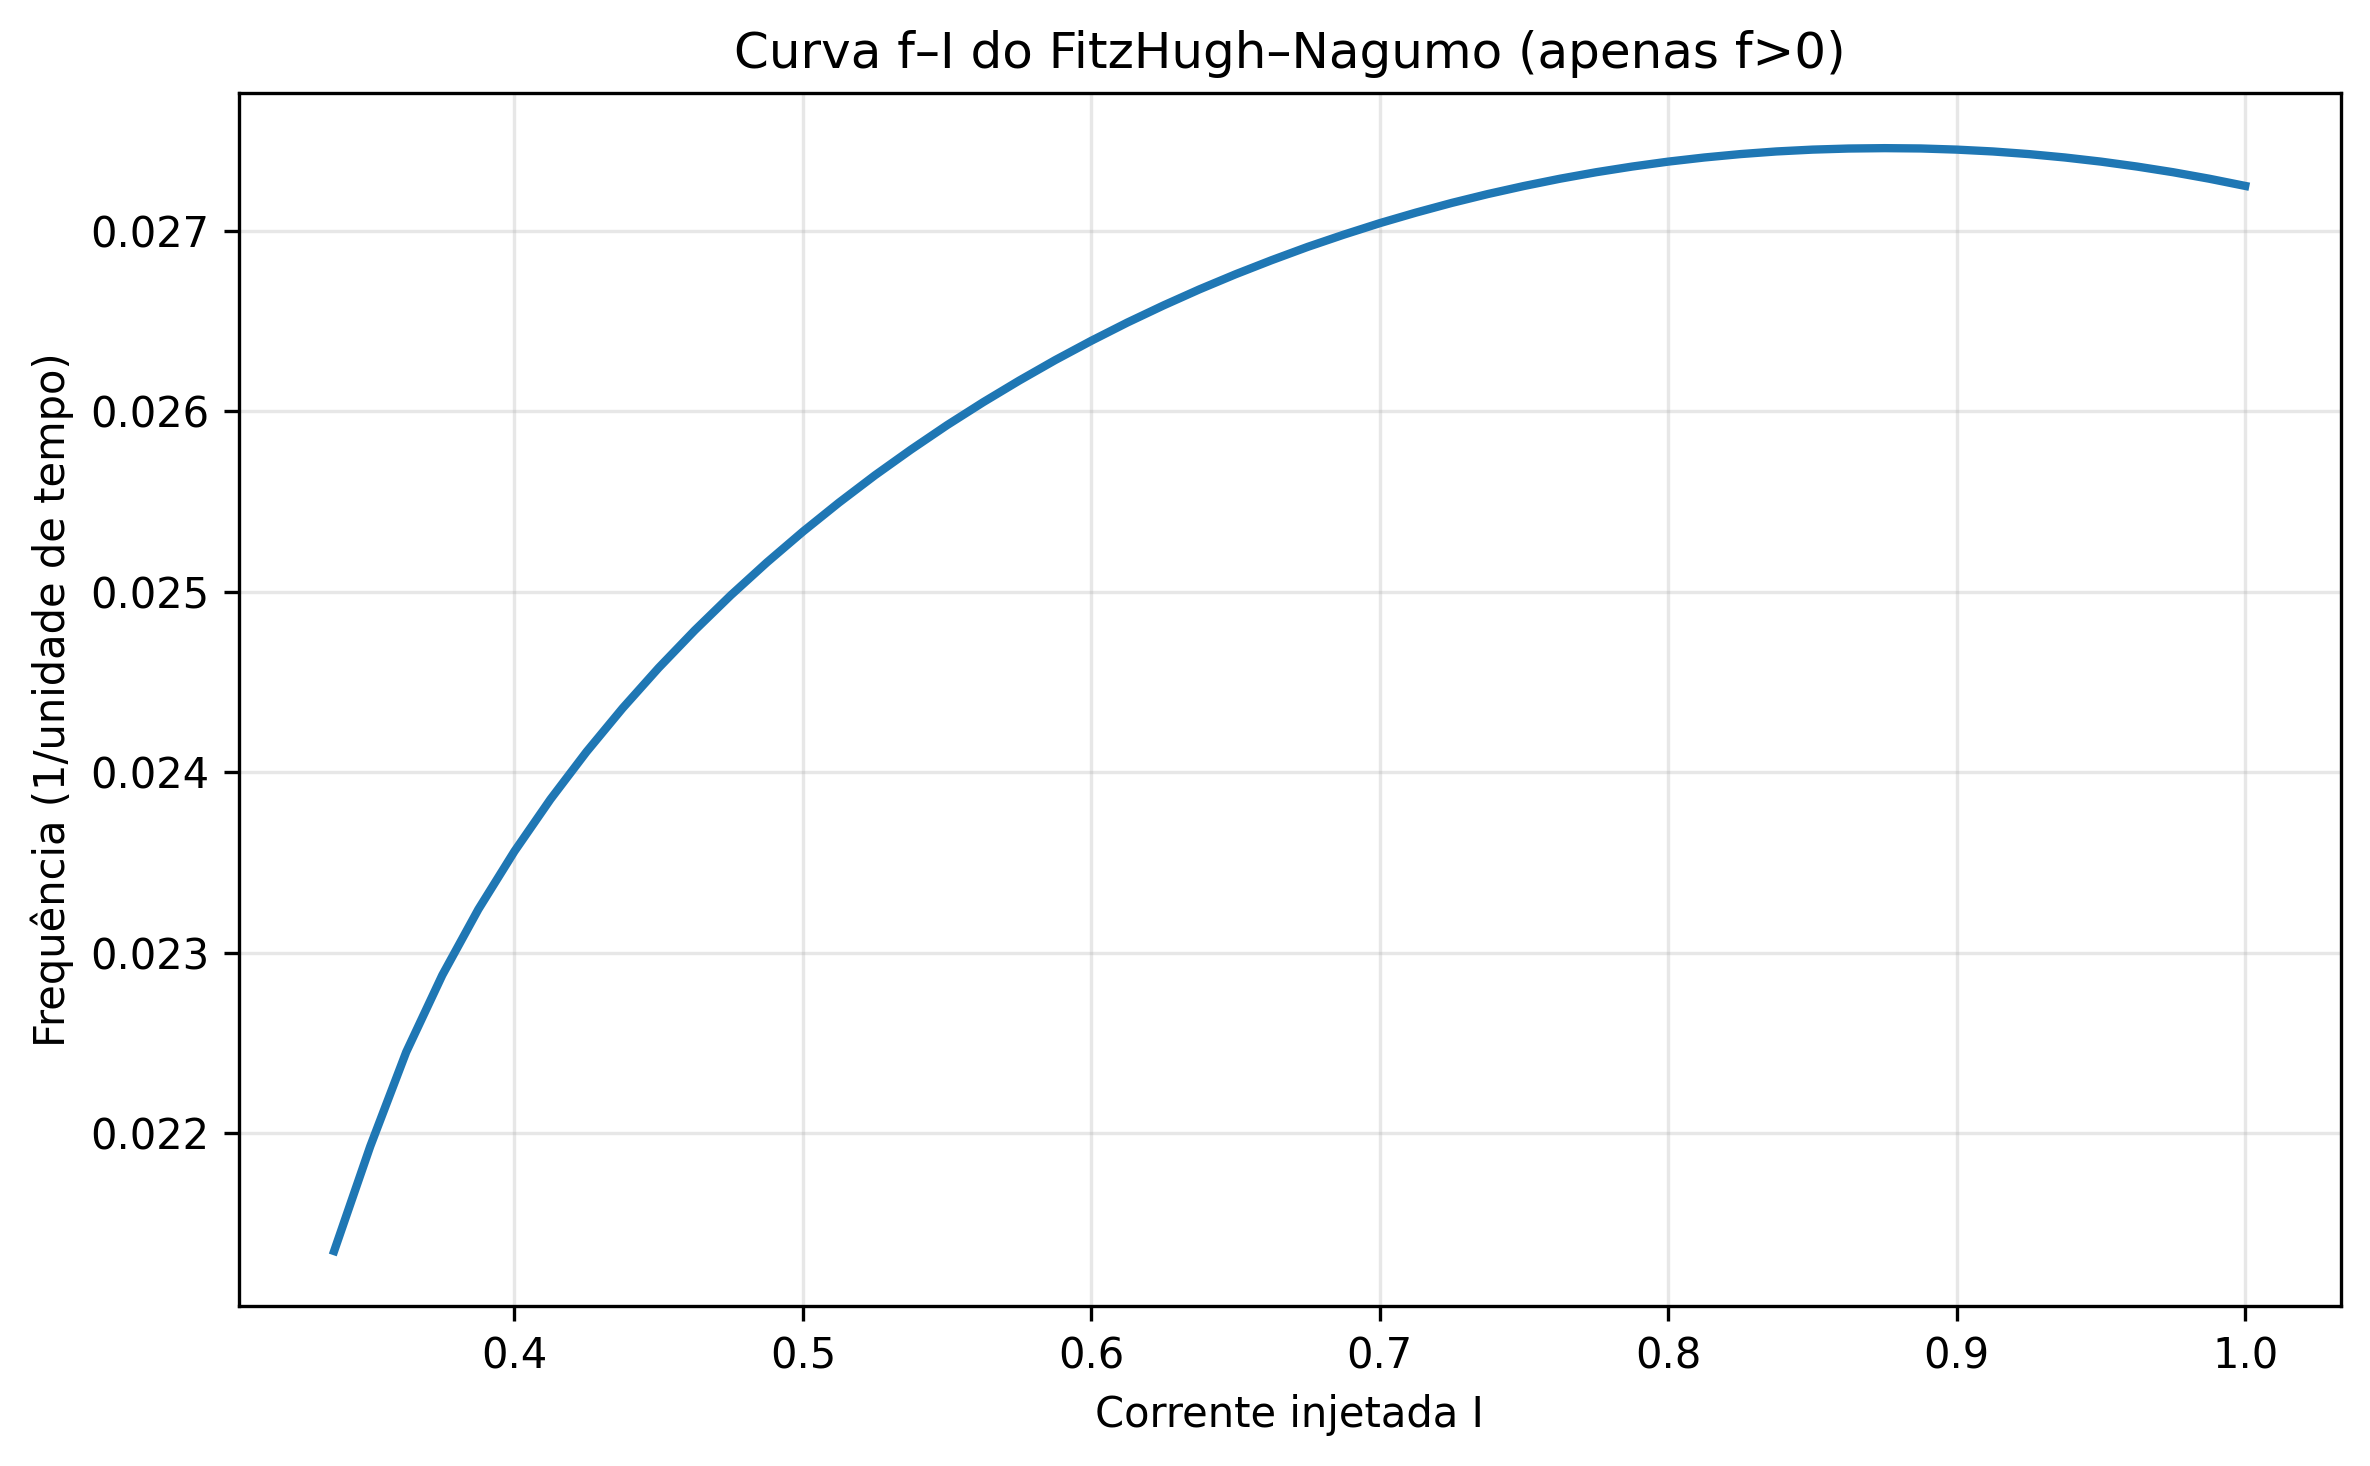
\includegraphics[width=11cm]{../figures/ex_1k.png}
		\caption{Curva f-I do modelo FitzHugh-Nagumo.}
	\end{figure}
	
	\noindent O modelo é de tipo 2, pois o módulo da frequência dá um salto em $I \approx 0.35$, sendo que antes disso ela é nula.\\\\
	
	\noindent\textbf{Questão 2.}
	
	\noindent\textbf{(a)} Obtenha as expressões para as nulclinas de $V_m$ e $n$ e gere um gráfico do espaço de fase $n$–$V_m$ mostrando essas nulclinas. Identifique o(s) ponto(s) fixo(s) do sistema e seu(s) tipo(s) de estabilidade.\\
	
	\noindent\textbf{Resposta:}
	
	\noindent\textit{Nulclinas, pontos fixos e estabilidade (parâmetros de Rinzel–Ermentrout e $J=15\,\mu\mathrm{A/cm}^2$).}
	
	\medskip
	O modelo é
	\[
	\begin{cases}
		C_m\,\dfrac{dV}{dt} \;=\; F(V,n) 
		= -\bar g_{\mathrm{Ca}}\,m_\infty(V)\,(V-E_{\mathrm{Ca}})
		- \bar g_{\mathrm K}\,n\,(V-E_{\mathrm K})
		- \bar g_{\mathrm L}\,(V-E_{\mathrm L})
		+ J,\\[6pt]
		\tau_n(V)\,\dfrac{dn}{dt} \;=\; G(V,n)
		= n_\infty(V)-n,
	\end{cases}
	\]
	com
	\[
	m_\infty(V)=\tfrac12\!\left(1+\tanh\dfrac{V+1}{15}\right),\quad
	n_\infty(V)=\tfrac12\!\left(1+\tanh\dfrac{V}{30}\right),\quad
	\tau_n(V)=\dfrac{5}{\cosh(V/60)}.
	\]
	
	\noindent As \textbf{nulclinas} são dadas por $dV/dt=0$ e $dn/dt=0$:
	
	\[
	\boxed{\; n = n_\infty(V) \;} \qquad (\text{nulclina de }n),
	\]
	
	\[
	\boxed{\;
		n \;=\; \dfrac{J - \bar g_{\mathrm{Ca}}\,m_\infty(V)\,(V-E_{\mathrm{Ca}})
			- \bar g_{\mathrm L}\,(V-E_{\mathrm L})}
		{\bar g_{\mathrm K}\,(V-E_{\mathrm K})}
		\;}\qquad (\text{nulclina de }V,\; V\neq E_{\mathrm K}).
	\]
	
	\medskip
	Os \textbf{pontos fixos} são as interseções das nulclinas. Para os parâmetros
	\[
	\bar g_{\mathrm{Ca}}=1.1,\quad \bar g_{\mathrm K}=2.0,\quad \bar g_{\mathrm L}=0.5,\quad
	E_{\mathrm{Ca}}=100\,\mathrm{mV},\ E_{\mathrm K}=-70\,\mathrm{mV},\ E_{\mathrm L}=-50\,\mathrm{mV},\ 
	C_m=1,
	\]
	e $J=15$, obtemos numericamente um único equilíbrio
	\[
	\boxed{\; V^\ast \approx -31.73\ \mathrm{mV},\qquad n^\ast = n_\infty(V^\ast)\approx 0.1076.\;}
	\]
	
	\noindent A \textbf{estabilidade} é dada pelos autovalores de
	\[
	J(V^\ast,n^\ast)=
	\begin{bmatrix}
		F_V & F_n\\ G_V & G_n
	\end{bmatrix}_{(V^\ast,n^\ast)},
	\]
	onde
	\[
	\begin{aligned}
		F_V &= \frac{-\bar g_{\mathrm{Ca}}\!\left(m_\infty'(V)(V-E_{\mathrm{Ca}})+m_\infty(V)\right)-\bar g_{\mathrm K}n-\bar g_{\mathrm L}}{C_m},\qquad
		&F_n &= \frac{-\bar g_{\mathrm K}(V-E_{\mathrm K})}{C_m},\\[4pt]
		G_V &= \frac{n_\infty'(V)}{\tau_n(V)},\qquad
		&G_n &= -\frac{1}{\tau_n(V)},
	\end{aligned}
	\]
	com
	\(
	m_\infty'(V)=\tfrac{1}{30}\,\mathrm{sech}^2\!\big((V+1)/15\big),\ 
	n_\infty'(V)=\tfrac{1}{60}\,\mathrm{sech}^2\!(V/30).
	\)
	Avaliando em $(V^\ast,n^\ast)$ resulta
	\[
	\lambda_{1,2}\approx -0.3256 \pm 0.3203\,i,
	\]
	isto é, \textbf{foco estável} (parte real negativa).
	
	\begin{figure}[H]
		\centering
		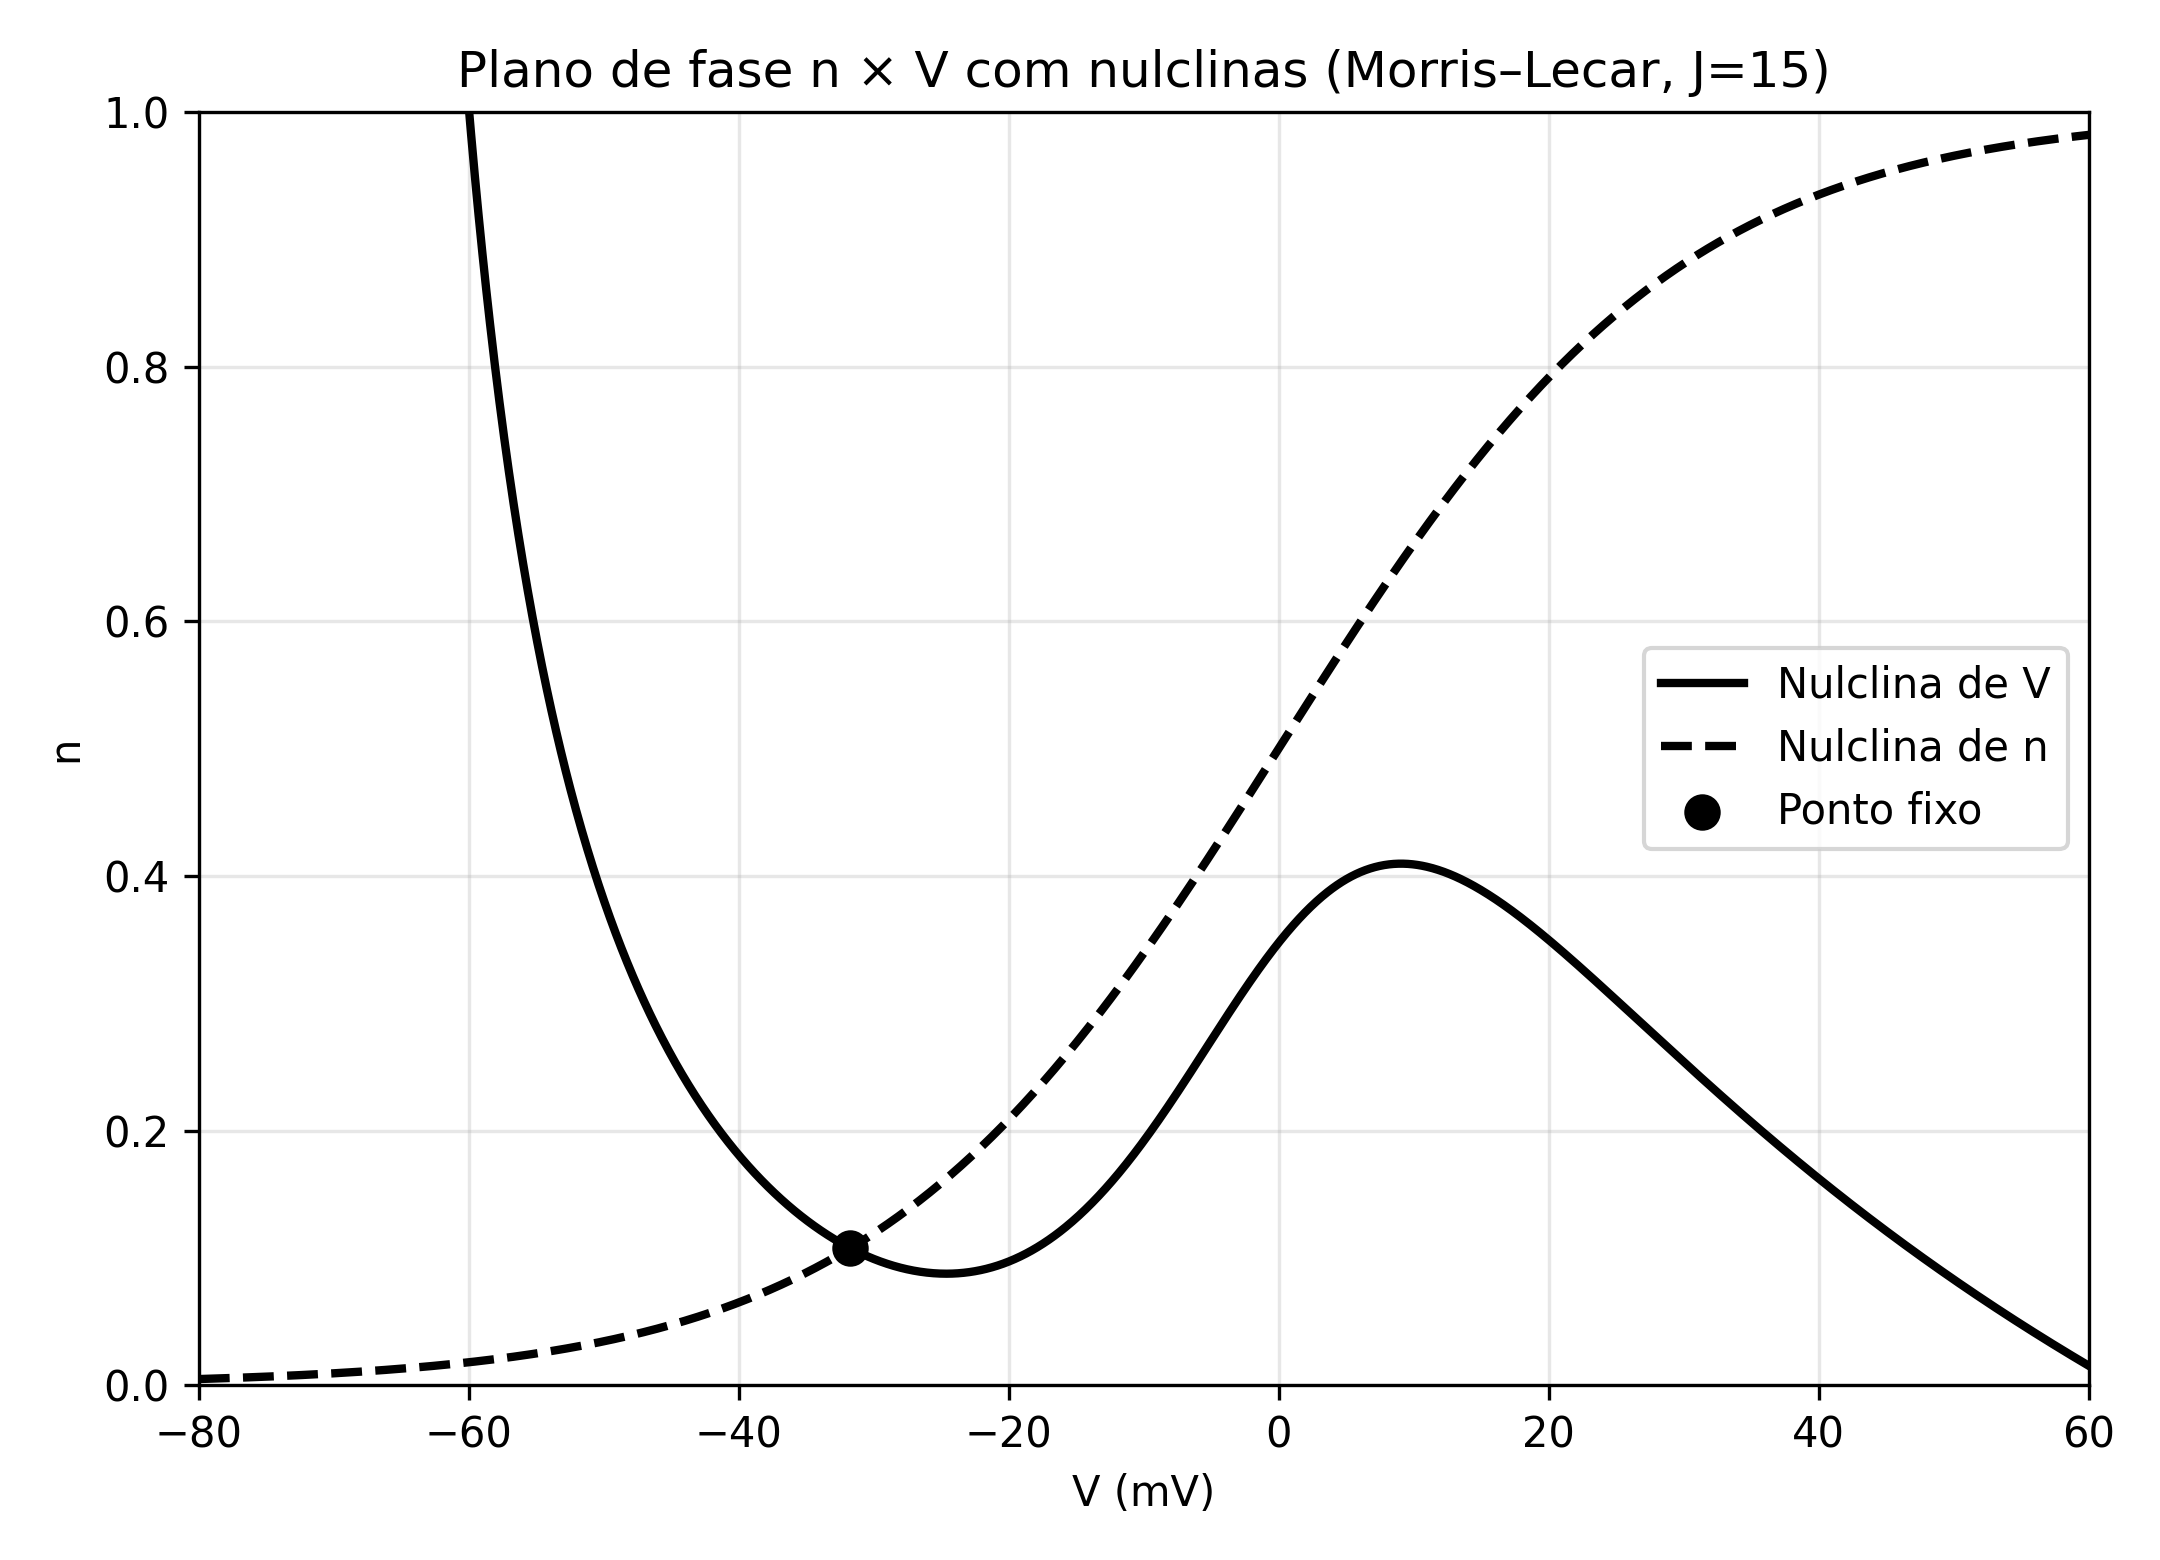
\includegraphics[width=11cm]{../figures/ex_2a.png}
		\caption{Nulclinas do modelo Morris-Lecar.}
	\end{figure}
	
	
	\noindent\textbf{(b)} Estude o efeito de pulsos instantâneos de corrente sobre o modelo de Morris-Lecar (como feito no item (h) da questão anterior). Para isso, simule as equações do modelo com os seguintes valores de $V_m$ como condição inicial $V_m(0)$: $-18$ mV, $-14{,}8$ mV, $-14{,}7$ mV e $-12$ mV. Use para $n(0)$ o valor de $n^*$ do ponto de equilíbrio encontrado no item anterior. Faça suas simulações durarem de $t = 0$ a $t = 20$ ms. Produza três gráficos com os dados de suas simulações: (i) um gráfico com as curvas de $V_m \times t$ para os quatro valores de $v(0)$ superpostas (cada curva indicada por uma cor ou símbolo diferente); (ii) um gráfico com as curvas de $n \times t$ para os quatro valores de $v(0)$ superpostas (cada curva indicada por uma cor ou símbolo diferente); (iii) um gráfico do plano de fase $n \times V_m$ mostrando as nulclinas de $V_m$ e $n$ (em cores ou símbolos diferentes) e as trajetórias correspondentes aos quatro casos simulados (também em cores ou símbolos diferentes).\\
	
	\noindent\textbf{Resposta:}
	
	\begin{figure}[H]
		\centering
		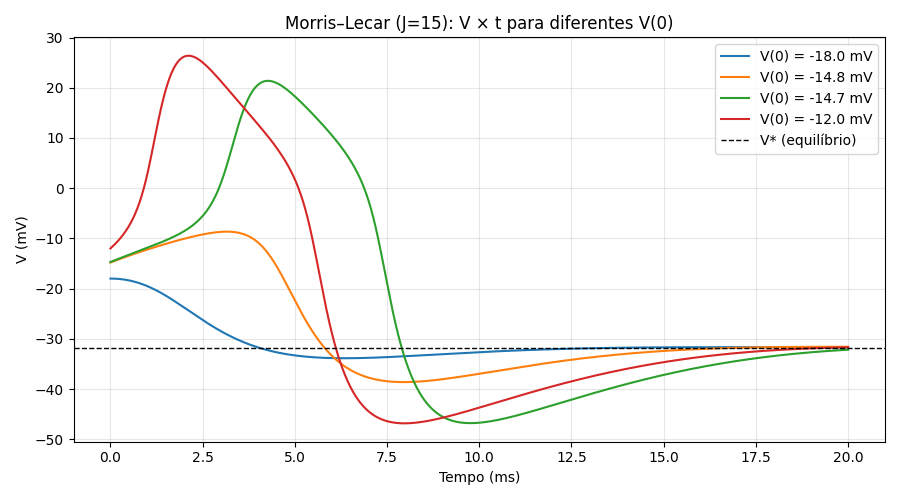
\includegraphics[width=11cm]{../figures/ex_2b_1.png}
		\caption{Gráfico de $V$ para diferentes $V(0)$ do modelo Morris-Lecar.}
	\end{figure}
	
	\begin{figure}[H]
		\centering
		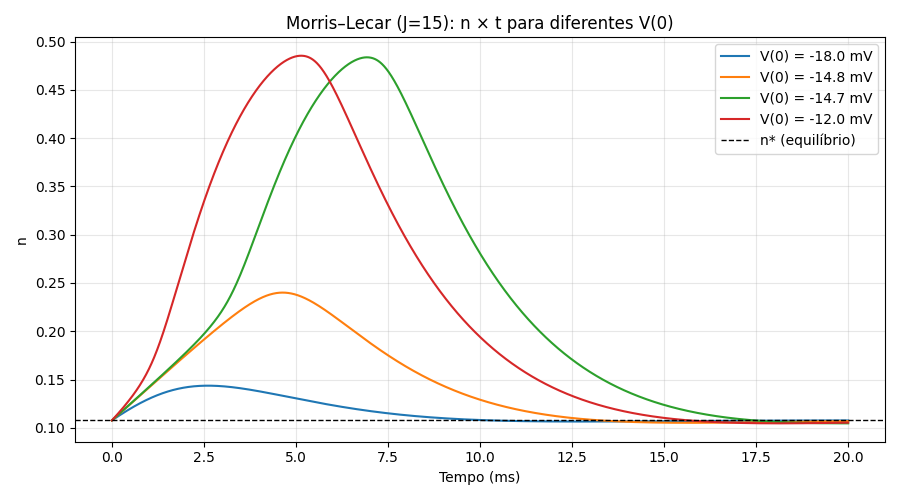
\includegraphics[width=11cm]{../figures/ex_2b_2.png}
		\caption{Gráfico de $n$ para diferentes $V(0)$ do modelo Morris-Lecar.}
	\end{figure}
	
	\begin{figure}[H]
		\centering
		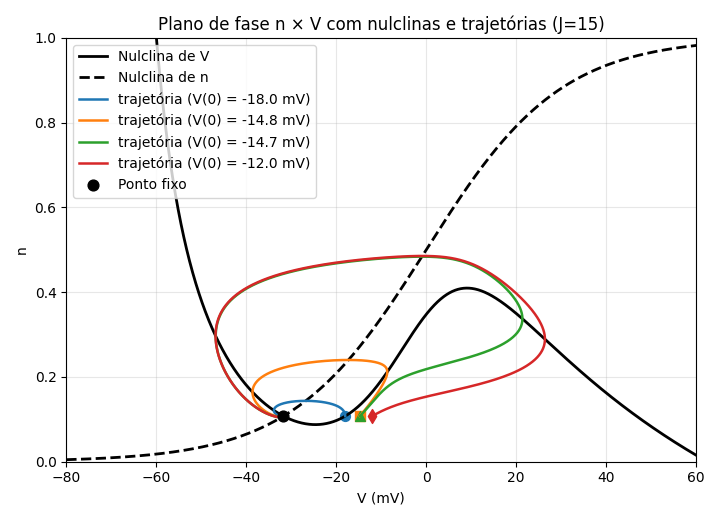
\includegraphics[width=11cm]{../figures/ex_2b_3.png}
		\caption{Plano de fase com trajetorias para diferentes $V(0)$ do modelo Morris-Lecar.}
	\end{figure}
	
	\noindent\textbf{(c)} Estude agora o efeito de correntes injetadas constantes (desconsiderando a corrente $J = 15~\mu$A/cm$^2$) sobre o modelo de Morris-Lecar. Faça uma varredura por valores de $J$ na equação (3) indo de $20~\mu$A/cm$^2$ a $40~\mu$A/cm$^2$ e construa a curva f–I do modelo. O modelo de Morris-Lecar, com os parâmetros dados, é de tipo I ou tipo II? Tente determinar o valor de $J$ para o qual as oscilações começam. Faça o gráfico de $V_m \times t$ para uma das simulações que produz um trem de disparos (à sua escolha). Como o modelo de Morris-Lecar se compara com o modelo de FitzHugh-Nagumo estudado na questão anterior? Para ajudar na sua resposta, construa gráficos do espaço de fase $n$–$V_m$ mostrando as nulclinas e as trajetórias do sistema para dois valores de $J$ (desconsiderando a corrente $J = 15~\mu$A/cm$^2$): $J = 24{,}8~\mu$A/cm$^2$ e $J = 25~\mu$A/cm$^2$.\\
	
	\noindent\textbf{Resposta:}
	
	\begin{figure}[H]
		\centering
		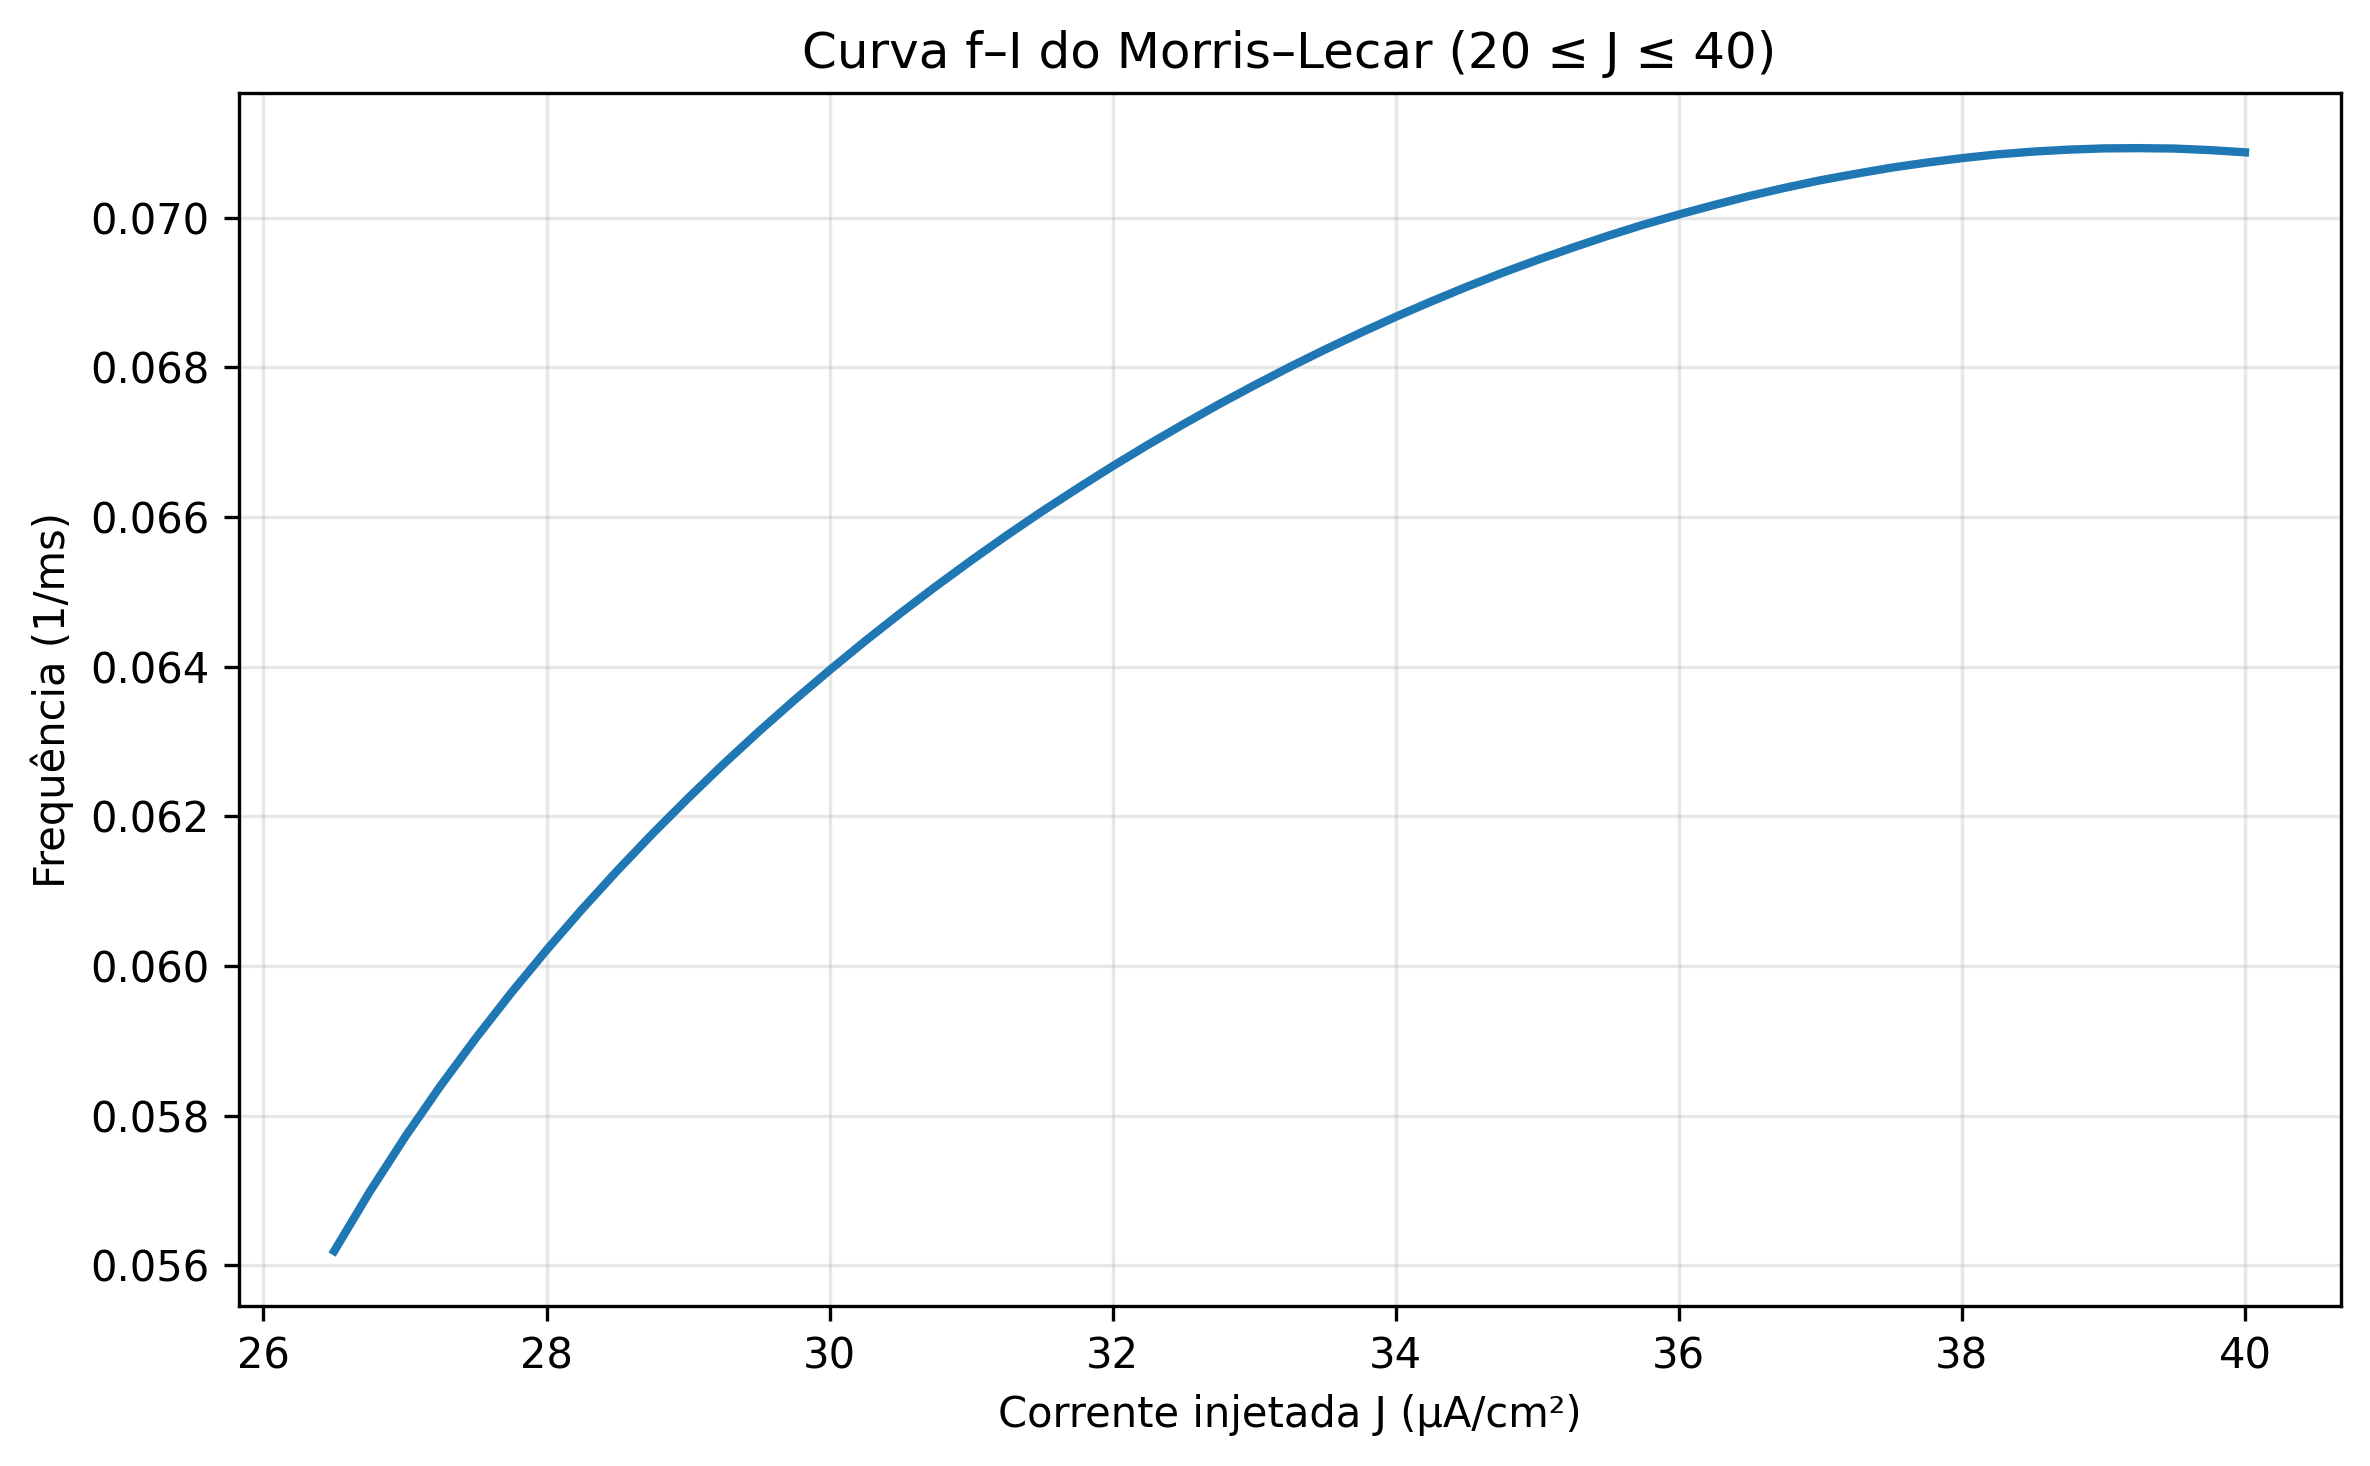
\includegraphics[width=11cm]{../figures/ex_2c_fI.png}
		\caption{Curva f-I do modelo Morris-Lecar.}
	\end{figure}
	
	\begin{figure}[H]
		\centering
		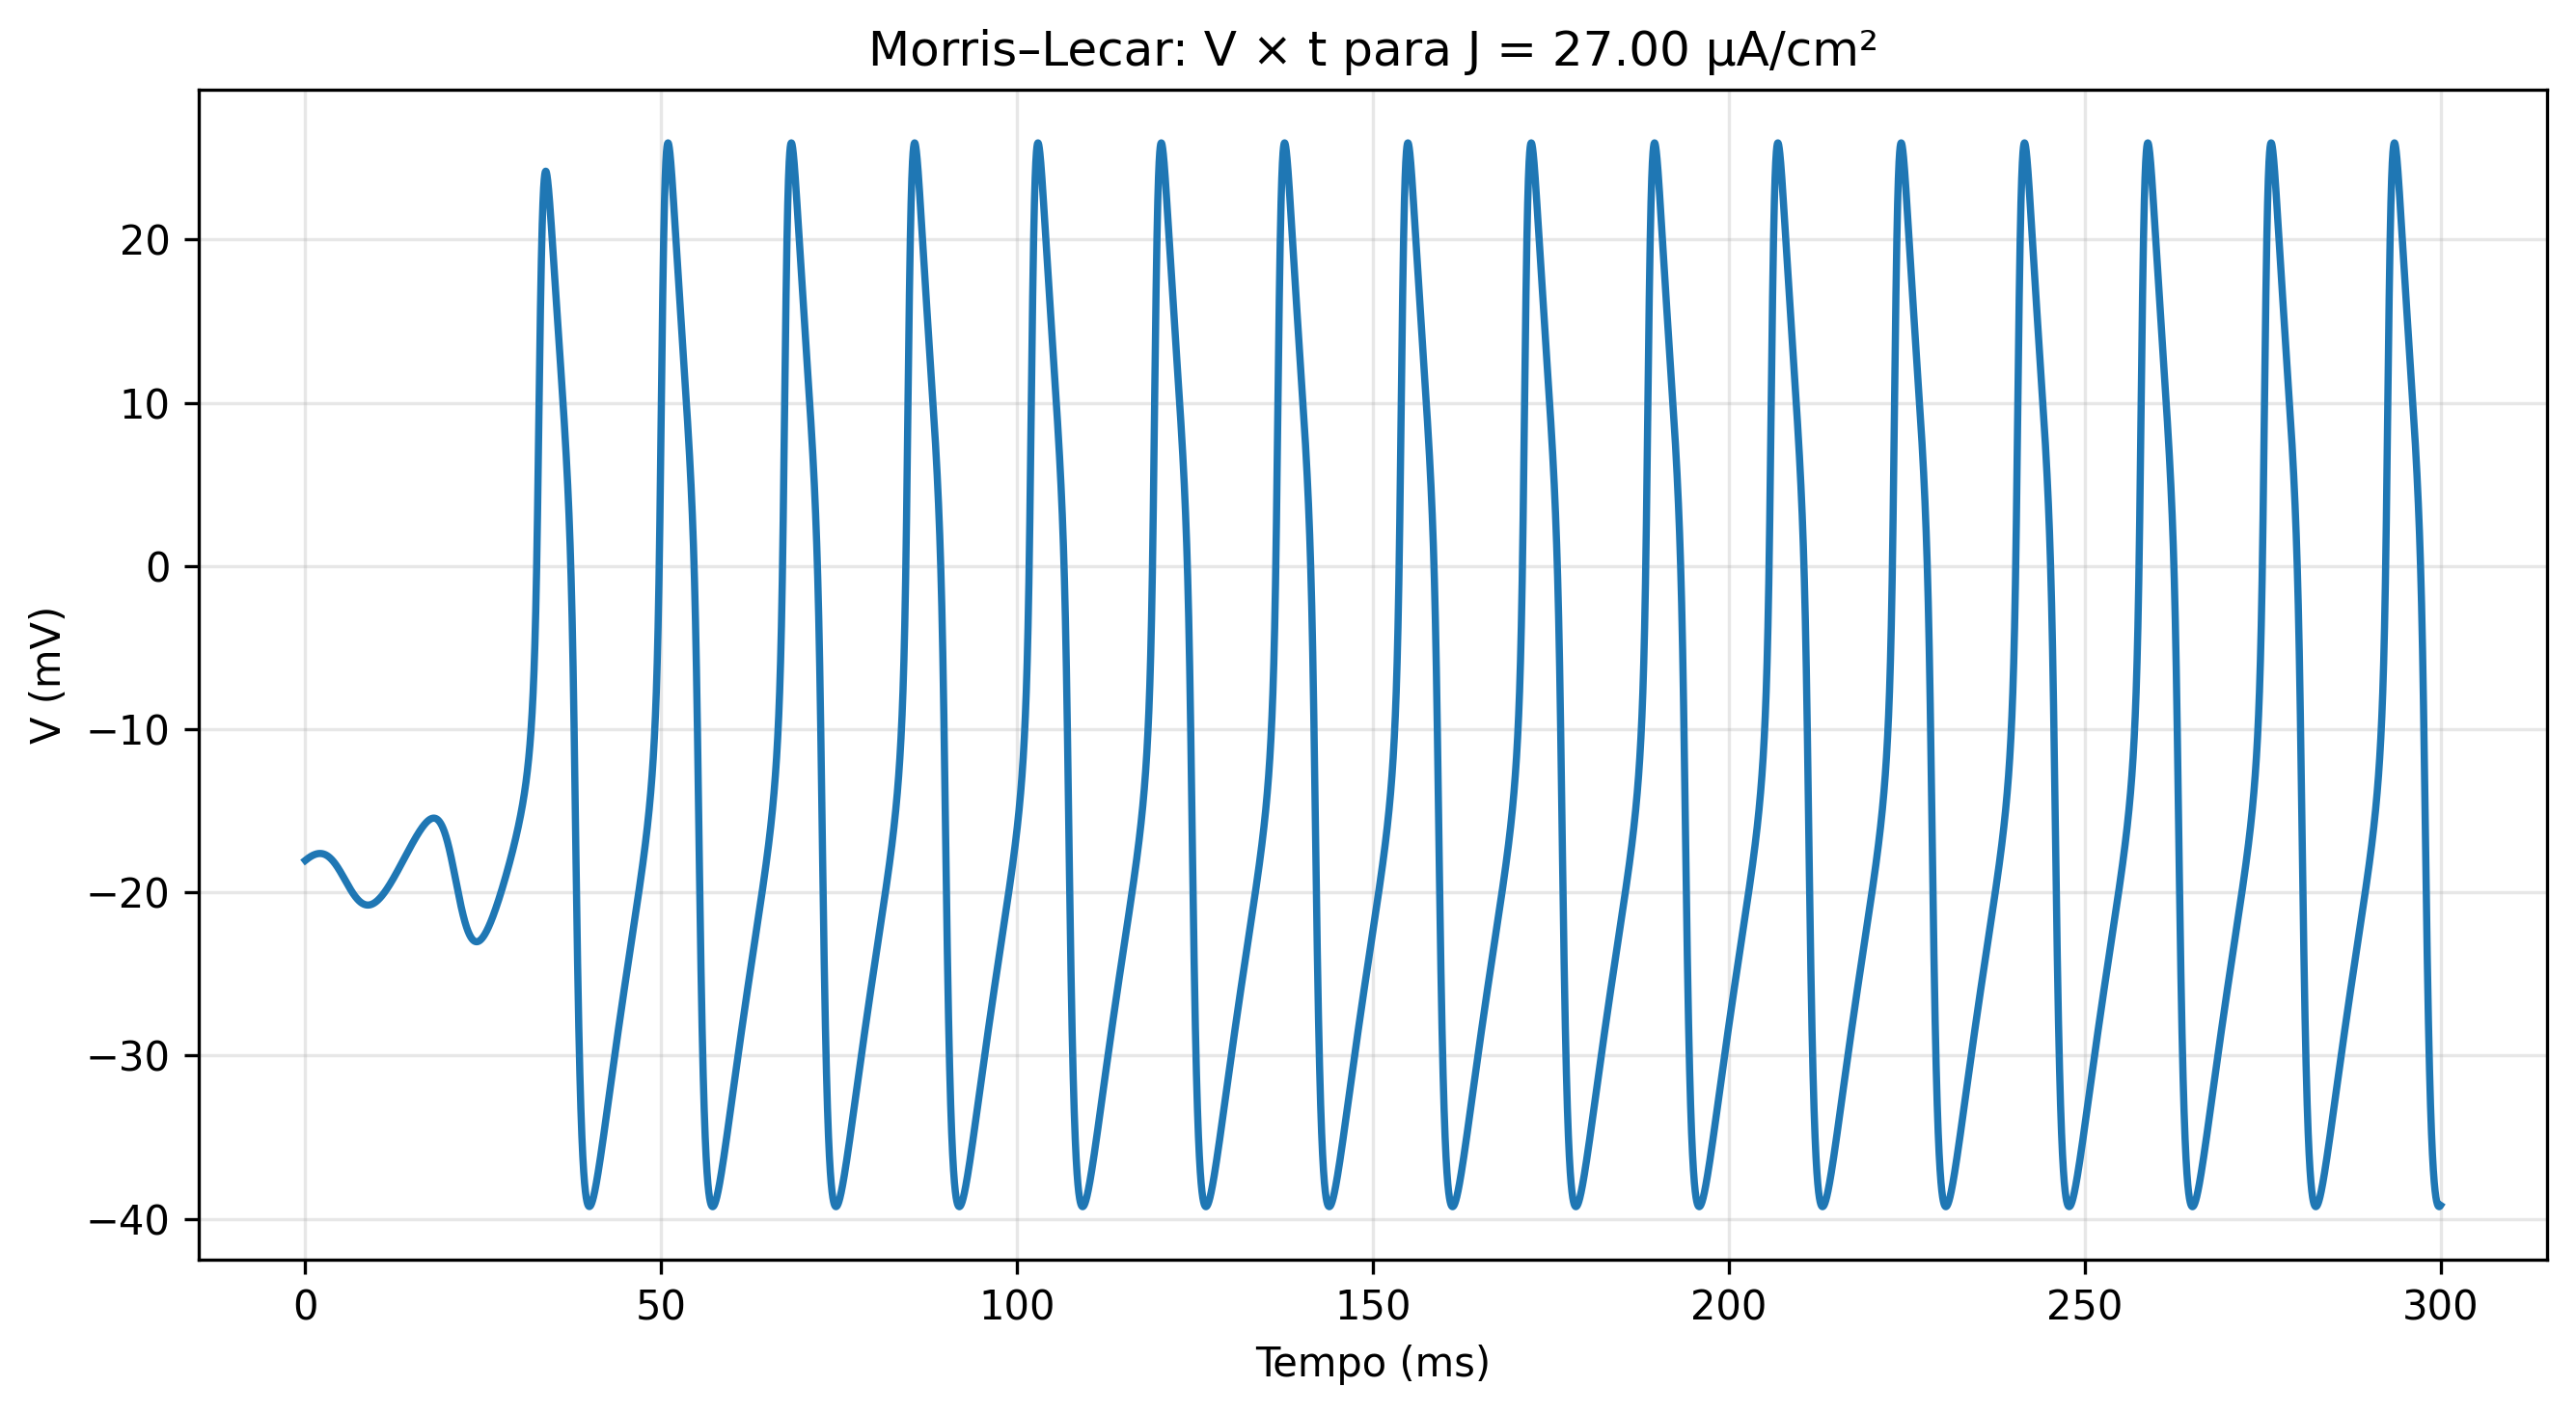
\includegraphics[width=11cm]{../figures/ex_2c_Vt.png}
		\caption{Trem de disparos do modelo Morris-Lecar.}
	\end{figure}
	
	\begin{figure}[H]
		\centering
		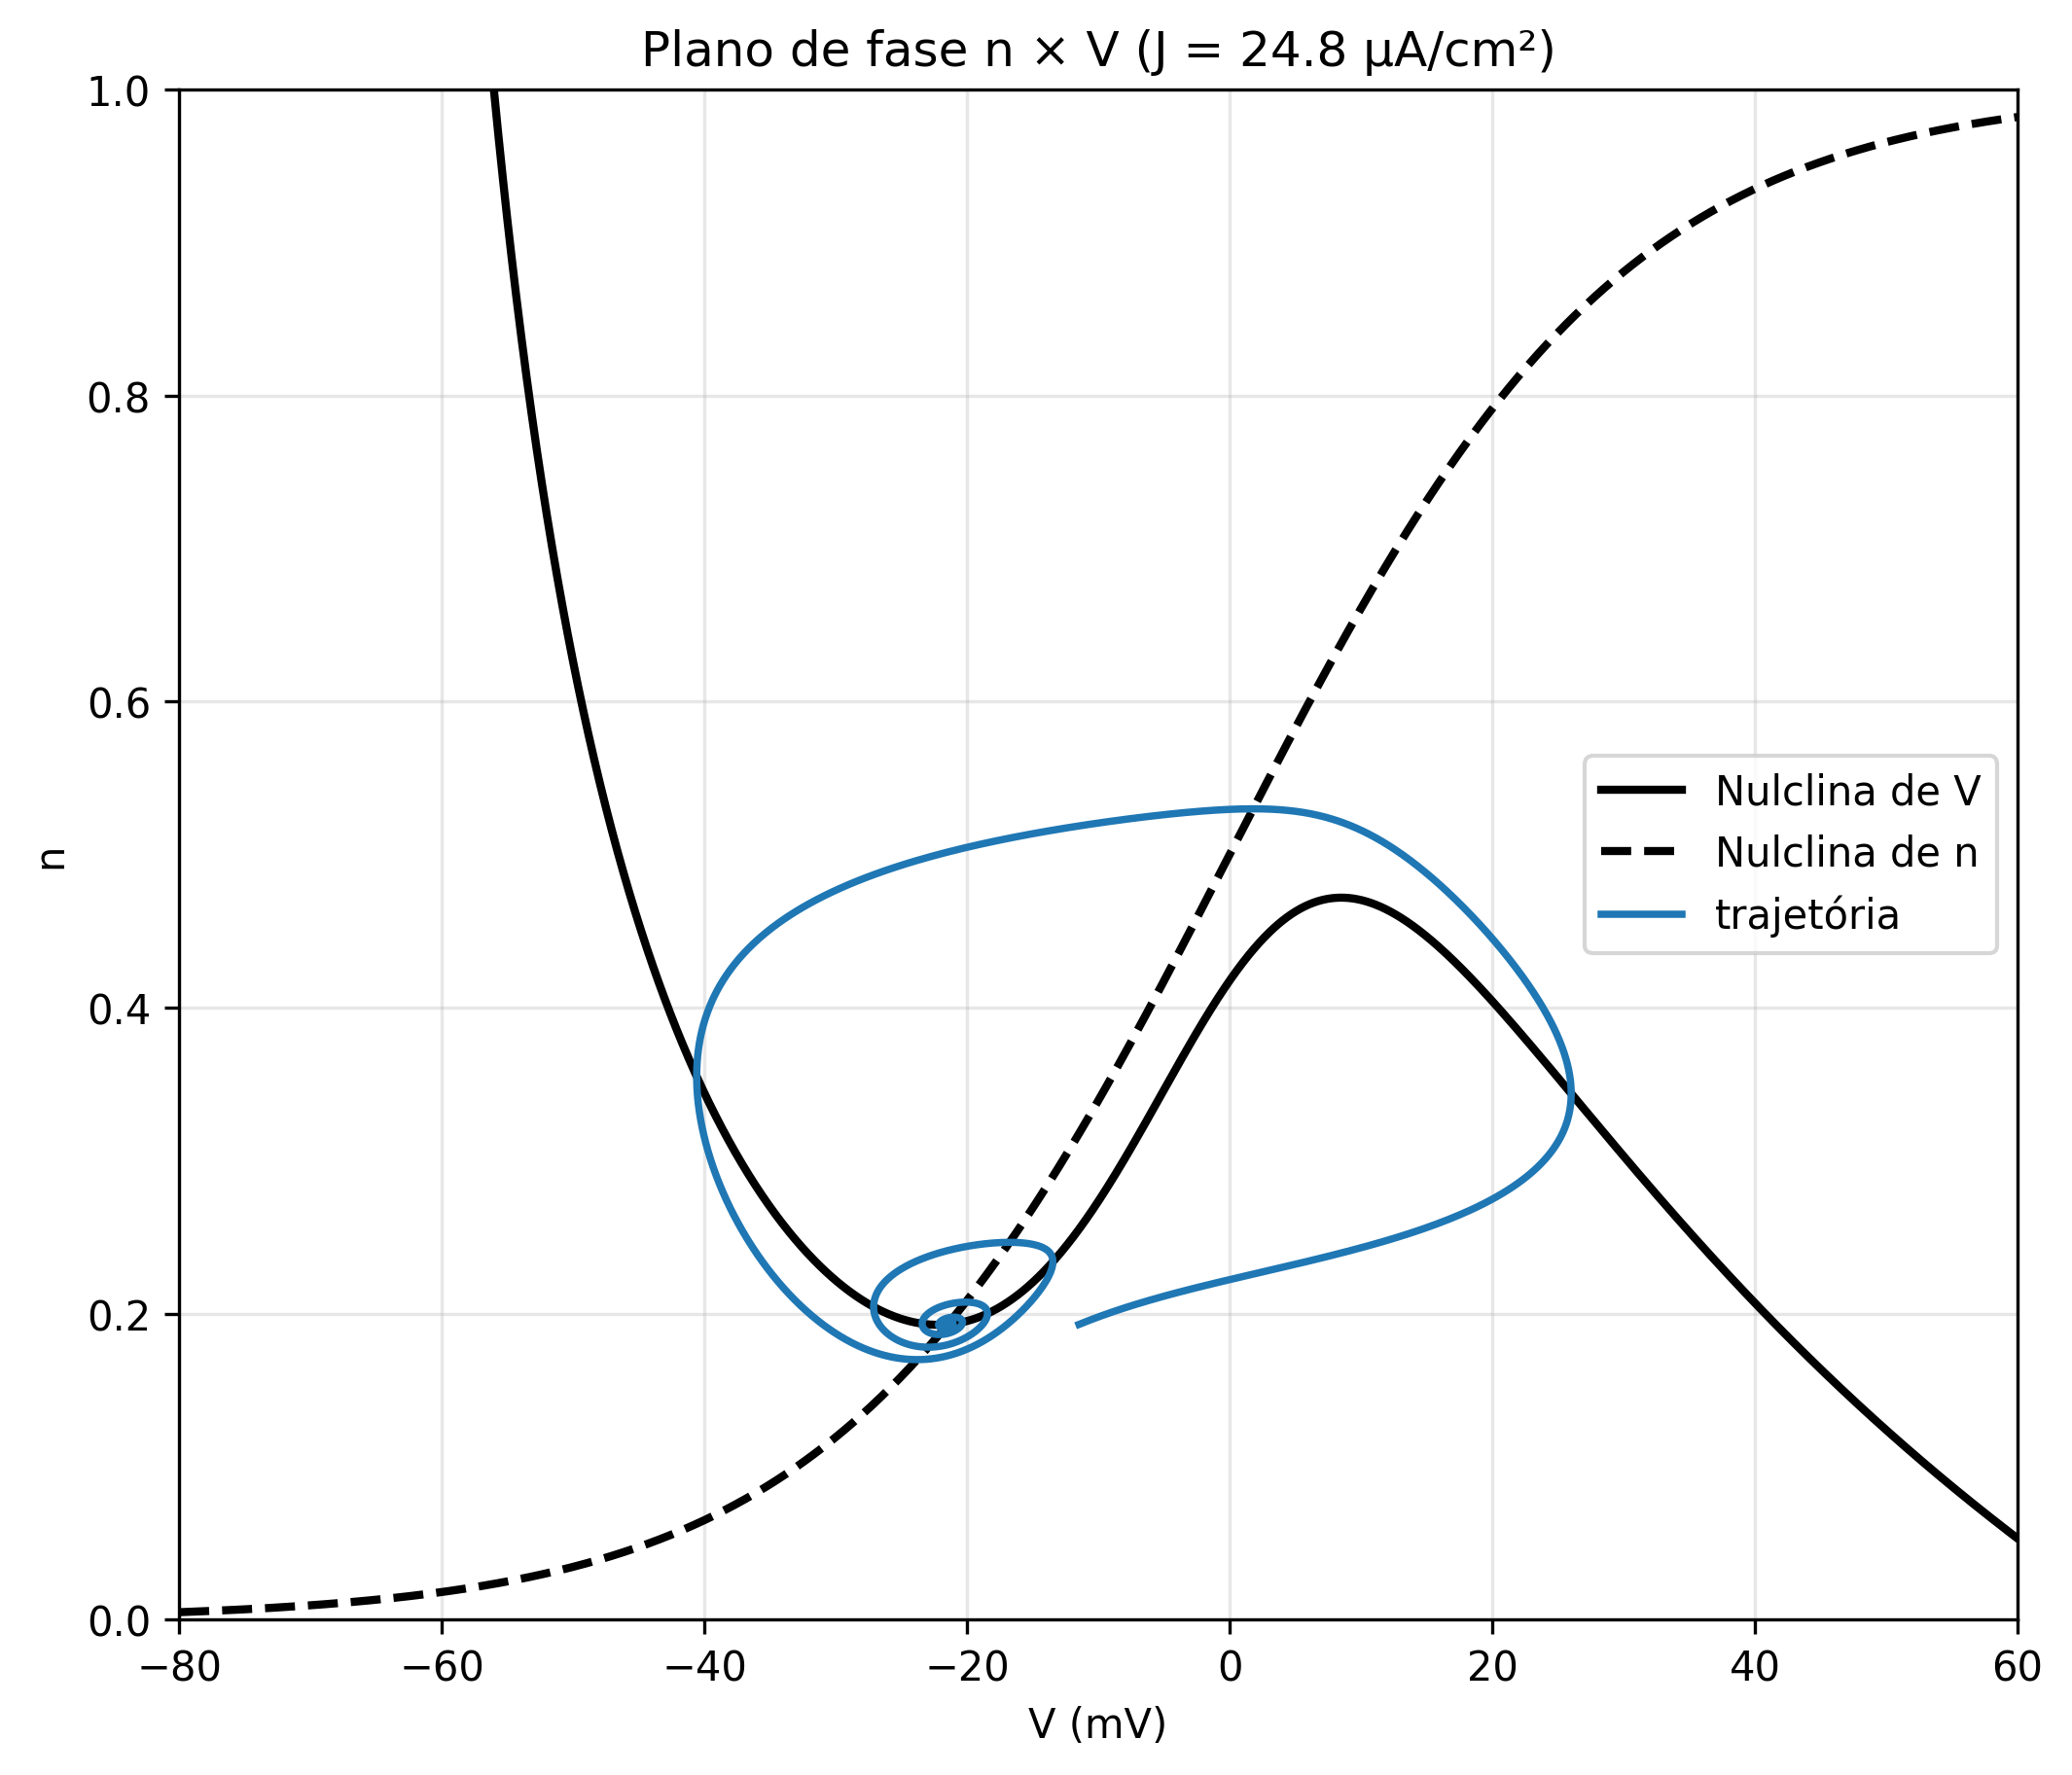
\includegraphics[width=11cm]{../figures/ex_2c_phase_J24p8.png}
		\caption{Trajetória do espaço de fase do modelo Morris-Lecar para $J = 24,8$ $\mu$A/cm$^2$.}
	\end{figure}
	
	\begin{figure}[H]
		\centering
		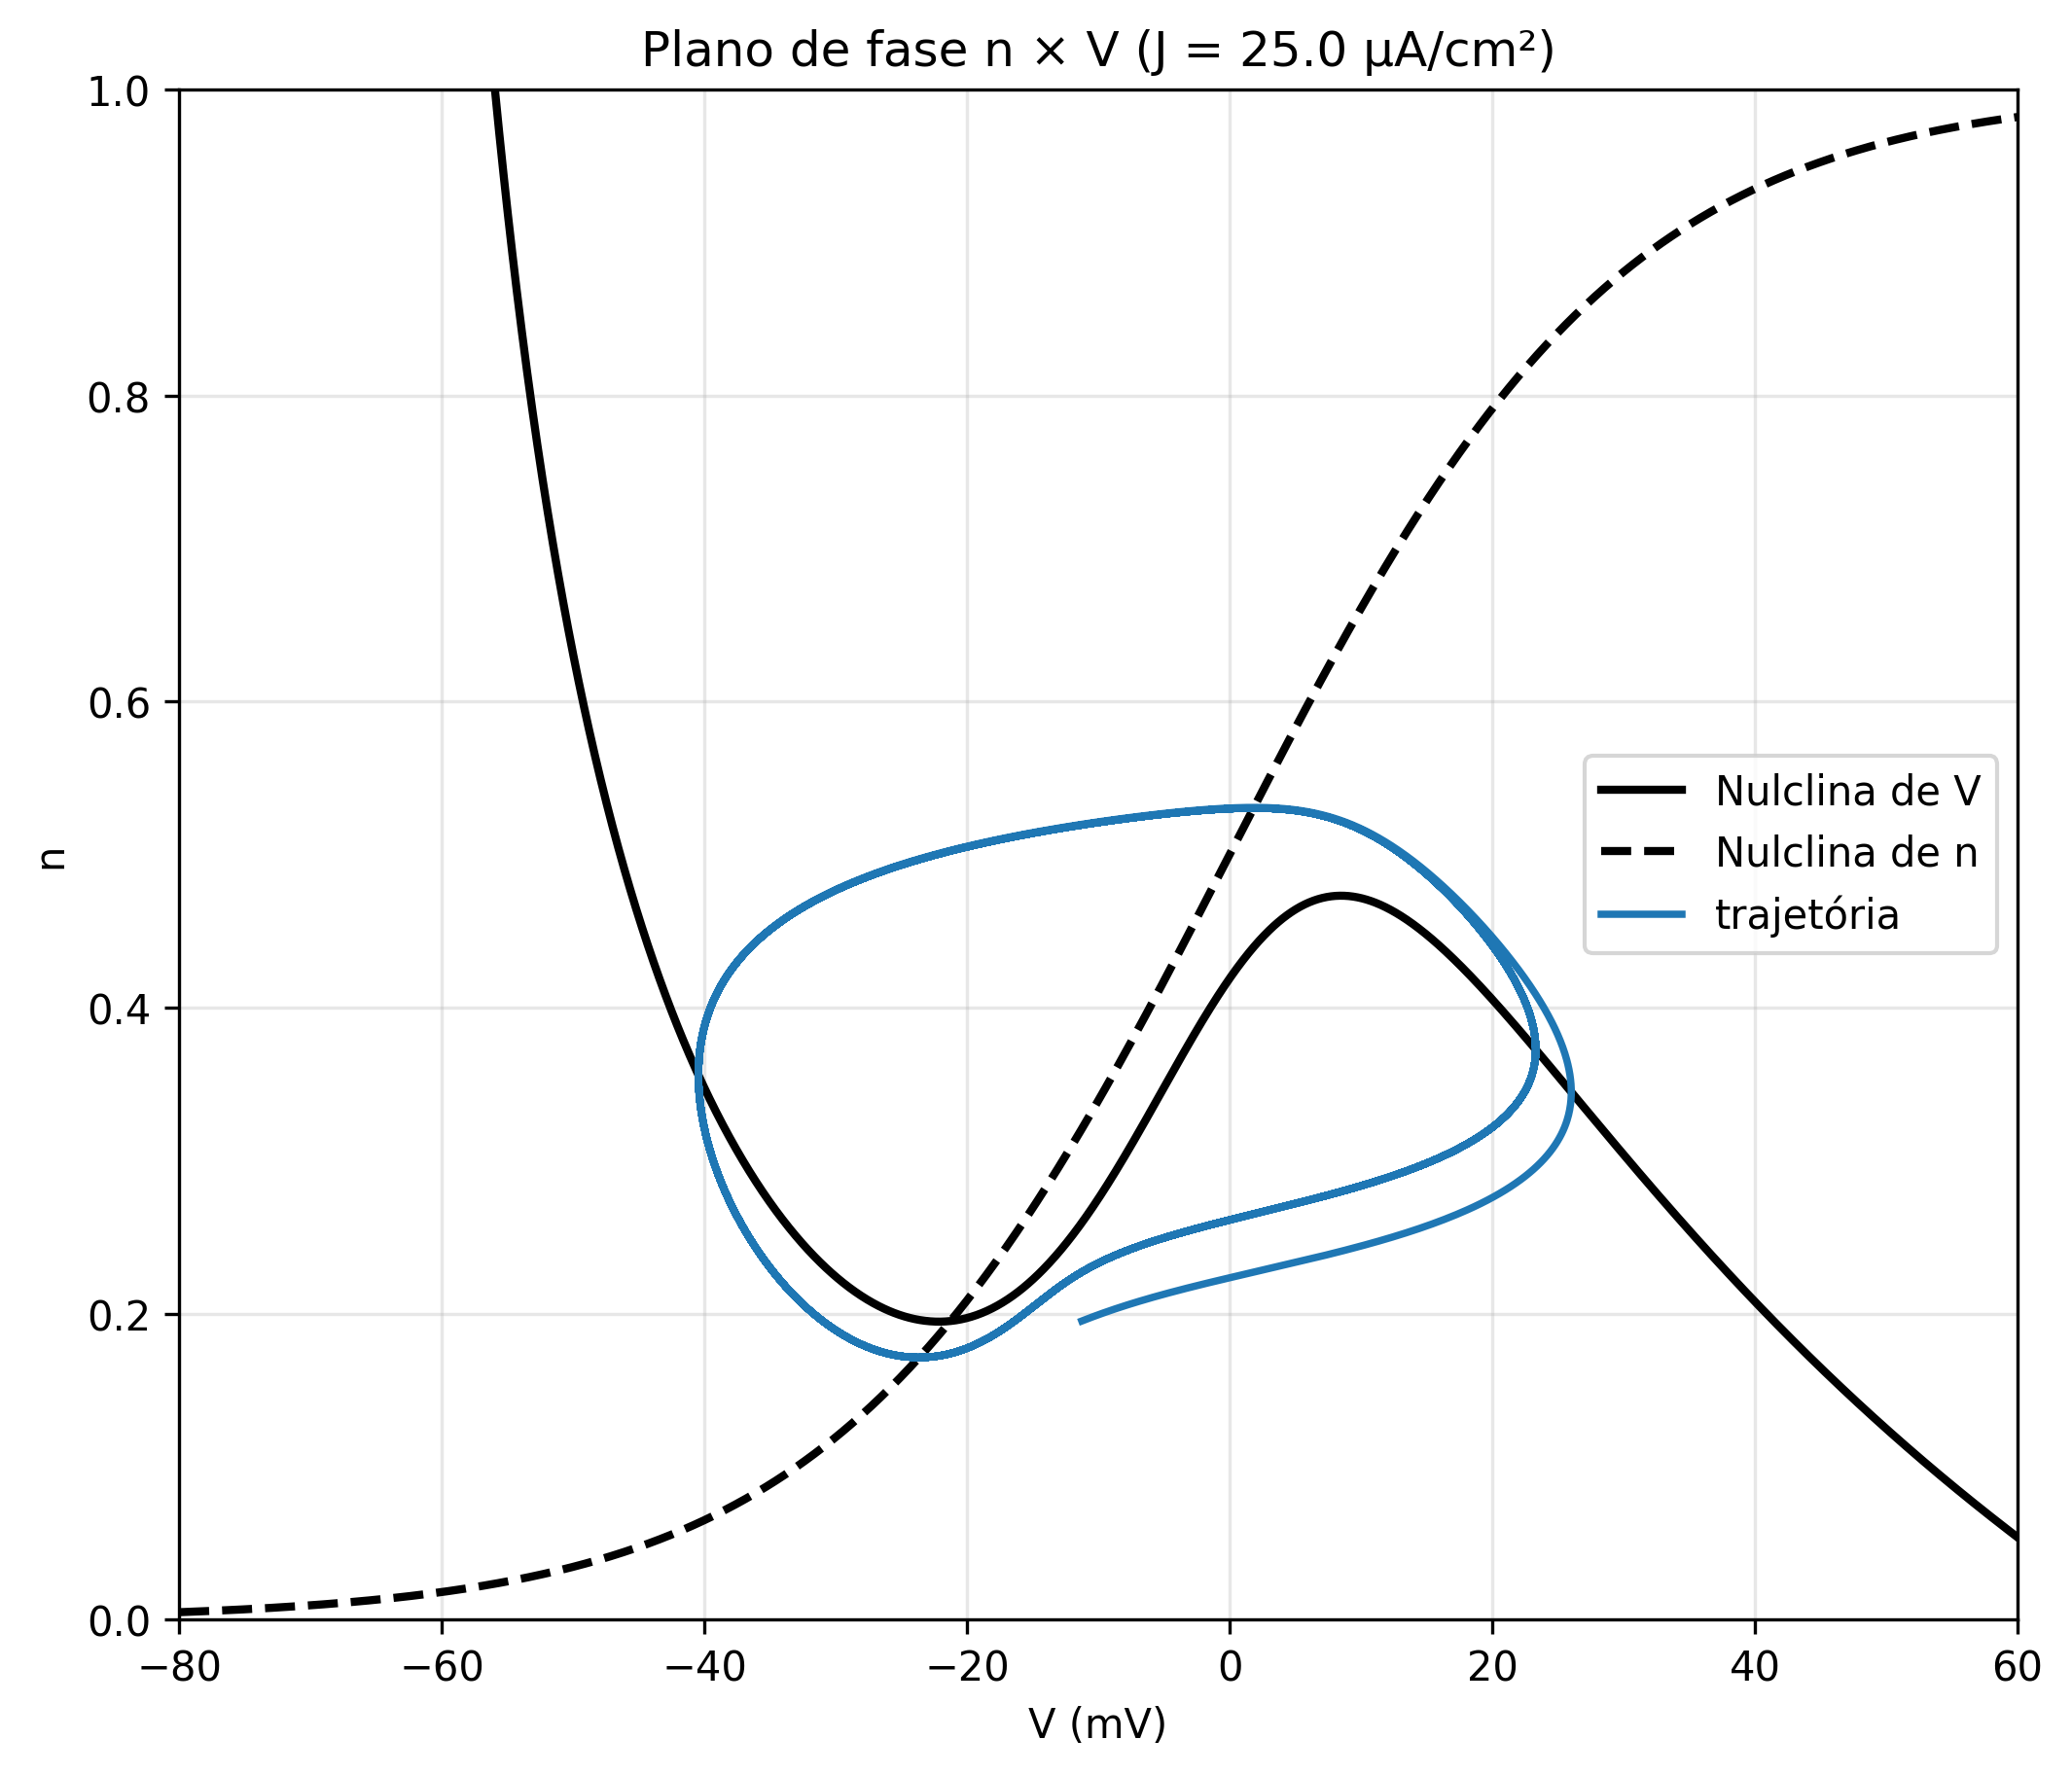
\includegraphics[width=11cm]{../figures/ex_2c_phase_J25p0.png}
		\caption{Trajetória do espaço de fase do modelo Morris-Lecar para $J = 24,8$ $\mu$A/cm$^2$.}
	\end{figure}
	
	
	
	
	Ambos os modelos estudados exibem retratos de fase qualitativamente equivalentes: dois tempos, foco que perde estabilidade por Hopf e ciclo-limite atrator; diferem sobretudo no desenho das nulclinas (cúbica+reta vs. N+sigmoide) e na geometria das trajetórias (FHN mais “quebrado”, ML mais suave).\\\\
	
	
	\noindent\textbf{(d)} Estude o modelo de Morris-Lecar com as seguintes modificações em relação ao que foi considerado acima. As funções que descrevem o valor estacionário e a constante de tempo da variável de ativação do potássio são modificadas para:
	\[
	n_{\infty}(V_m) = 0{,}5 \left( 1 + \tanh \frac{V_m - 10}{14{,}5} \right),
	\]
	\[
	\tau_n = \frac{3}{\cosh \frac{V_m - 10}{29}}.
	\]
	Mude também a densidade de condutância máxima do cálcio para $\bar{g}_{\text{Ca}} = 1$ mS/cm$^2$. Todos os demais parâmetros do modelo devem permanecer como estavam nos itens anteriores (sem a corrente de ajuste $J = 15~\mu$A/cm$^2$). Faça os gráficos das nulclinas de $V_m$ e $n$ para o modelo de Morris-Lecar modificado no seu espaço de fase. Identifique o(s) ponto(s) fixo(s) e seu(s) tipo(s) de estabilidade.\\
	
	\noindent\textbf{Resposta:}
	
	\noindent\textit{Morris–Lecar modificado (sem $J=15$).}
	
	\[
	m_\infty(V)=\tfrac12\!\left(1+\tanh\dfrac{V+1}{15}\right),\qquad
	n_\infty(V)=\tfrac12\!\left(1+\tanh\dfrac{V-10}{14.5}\right),\qquad
	\tau_n(V)=\dfrac{3}{\cosh\!\left(\dfrac{V-10}{29}\right)}.
	\]
	
	Com \( \bar g_{\mathrm{Ca}}=1.0\,\mathrm{mS/cm}^2\), \( \bar g_{\mathrm K}=2.0\), \( \bar g_{\mathrm L}=0.5\),
	\(E_{\mathrm{Ca}}=100\,\mathrm{mV}\), \(E_{\mathrm K}=-70\,\mathrm{mV}\), \(E_{\mathrm L}=-50\,\mathrm{mV}\), \(C_m=1\), e \(J=0\).
	
	As \textbf{nulclinas} são:
	
	\[
	\boxed{\, n=n_\infty(V) \,}\qquad(\text{nulclina de }n),
	\]
	
	\[
	\boxed{\, n=\dfrac{-\,\bar g_{\mathrm{Ca}}\,m_\infty(V)\,(V-E_{\mathrm{Ca}})
			-\bar g_{\mathrm L}(V-E_{\mathrm L})}{\bar g_{\mathrm K}(V-E_{\mathrm K})} \,}\qquad(\text{nulclina de }V,\;V\neq E_{\mathrm K}).
	\]
	
	\noindent O(s) ponto(s) de equilíbrio $(V^*,n^*)$ são obtidos pela interseção das nulclinas, isto é,
	\[
	n_\infty(V^*) = \dfrac{-\,\bar g_{\mathrm{Ca}}\,m_\infty(V^*)\,(V^*-E_{\mathrm{Ca}})
		-\bar g_{\mathrm L}(V^*-E_{\mathrm L})}{\bar g_{\mathrm K}(V^*-E_{\mathrm K})}.
	\]
	
	Para cada ponto fixo, a estabilidade é dada pelos autovalores da jacobiana:
	\[
	J=\begin{bmatrix}
		F_V & F_n\\[2pt] G_V & G_n
	\end{bmatrix},\quad
	\begin{aligned}
		F_V&=\frac{-\bar g_{\mathrm{Ca}}\!\big(m_\infty'(V)(V-E_{\mathrm{Ca}})+m_\infty(V)\big)-\bar g_{\mathrm K}n-\bar g_{\mathrm L}}{C_m},\\[2pt]
		F_n&=\frac{-\bar g_{\mathrm K}(V-E_{\mathrm K})}{C_m},\\[2pt]
		G_V&=\frac{n_\infty'(V)}{\tau_n(V)},\qquad
		G_n=-\frac{1}{\tau_n(V)}.
	\end{aligned}
	\]
	
	\noindent A classificação segue pelo traço e determinante:
	\[
	\tau = F_V + G_n,\qquad
	\Delta = F_VG_n - F_nG_V,
	\]
	onde:
	\[
	\begin{cases}
		\Delta<0 &\Rightarrow \text{sela (instável)},\\
		\Delta>0,\ \tau<0 &\Rightarrow \text{nó/foco estável},\\
		\Delta>0,\ \tau>0 &\Rightarrow \text{nó/foco instável},\\
		\tau=0 &\Rightarrow \text{Hopf (limiar)}.
	\end{cases}
	\]
	
	\vspace{1em}
	\noindent\textbf{Resultados numéricos obtidos:}
	
	\begin{center}
		\begin{tabular}{c c c c c}
			\toprule
			Equilíbrio & $V^*$ (mV) & $n^*$ & Tipo & Autovalores \\ 
			\midrule
			1 & $-49{,}56$ & $0{,}0003$ & Nó estável & $[-1{,}32,\ -0{,}47]$ \\
			2 & $-7{,}90$  & $0{,}078$  & Sela (instável) & $[1{,}76,\ -0{,}17]$ \\
			3 & $0{,}14$   & $0{,}204$  & Nó instável & $[1{,}10,\ 0{,}41]$ \\
			\bottomrule
		\end{tabular}
	\end{center}
	
	\noindent Assim, o modelo modificado apresenta \textbf{três pontos de equilíbrio}:
	um nó estável em potenciais hiperpolarizados, uma sela intermediária e um nó instável próximo de zero volts.
	Essa estrutura é típica de sistemas excitatórios com dinâmica bistável — indicando que, para pequenas correntes injetadas,
	perturbações podem deslocar o sistema de um regime estacionário estável para trajetórias excitatórias transitórias.
	
	
	\begin{figure}[H]
		\centering
		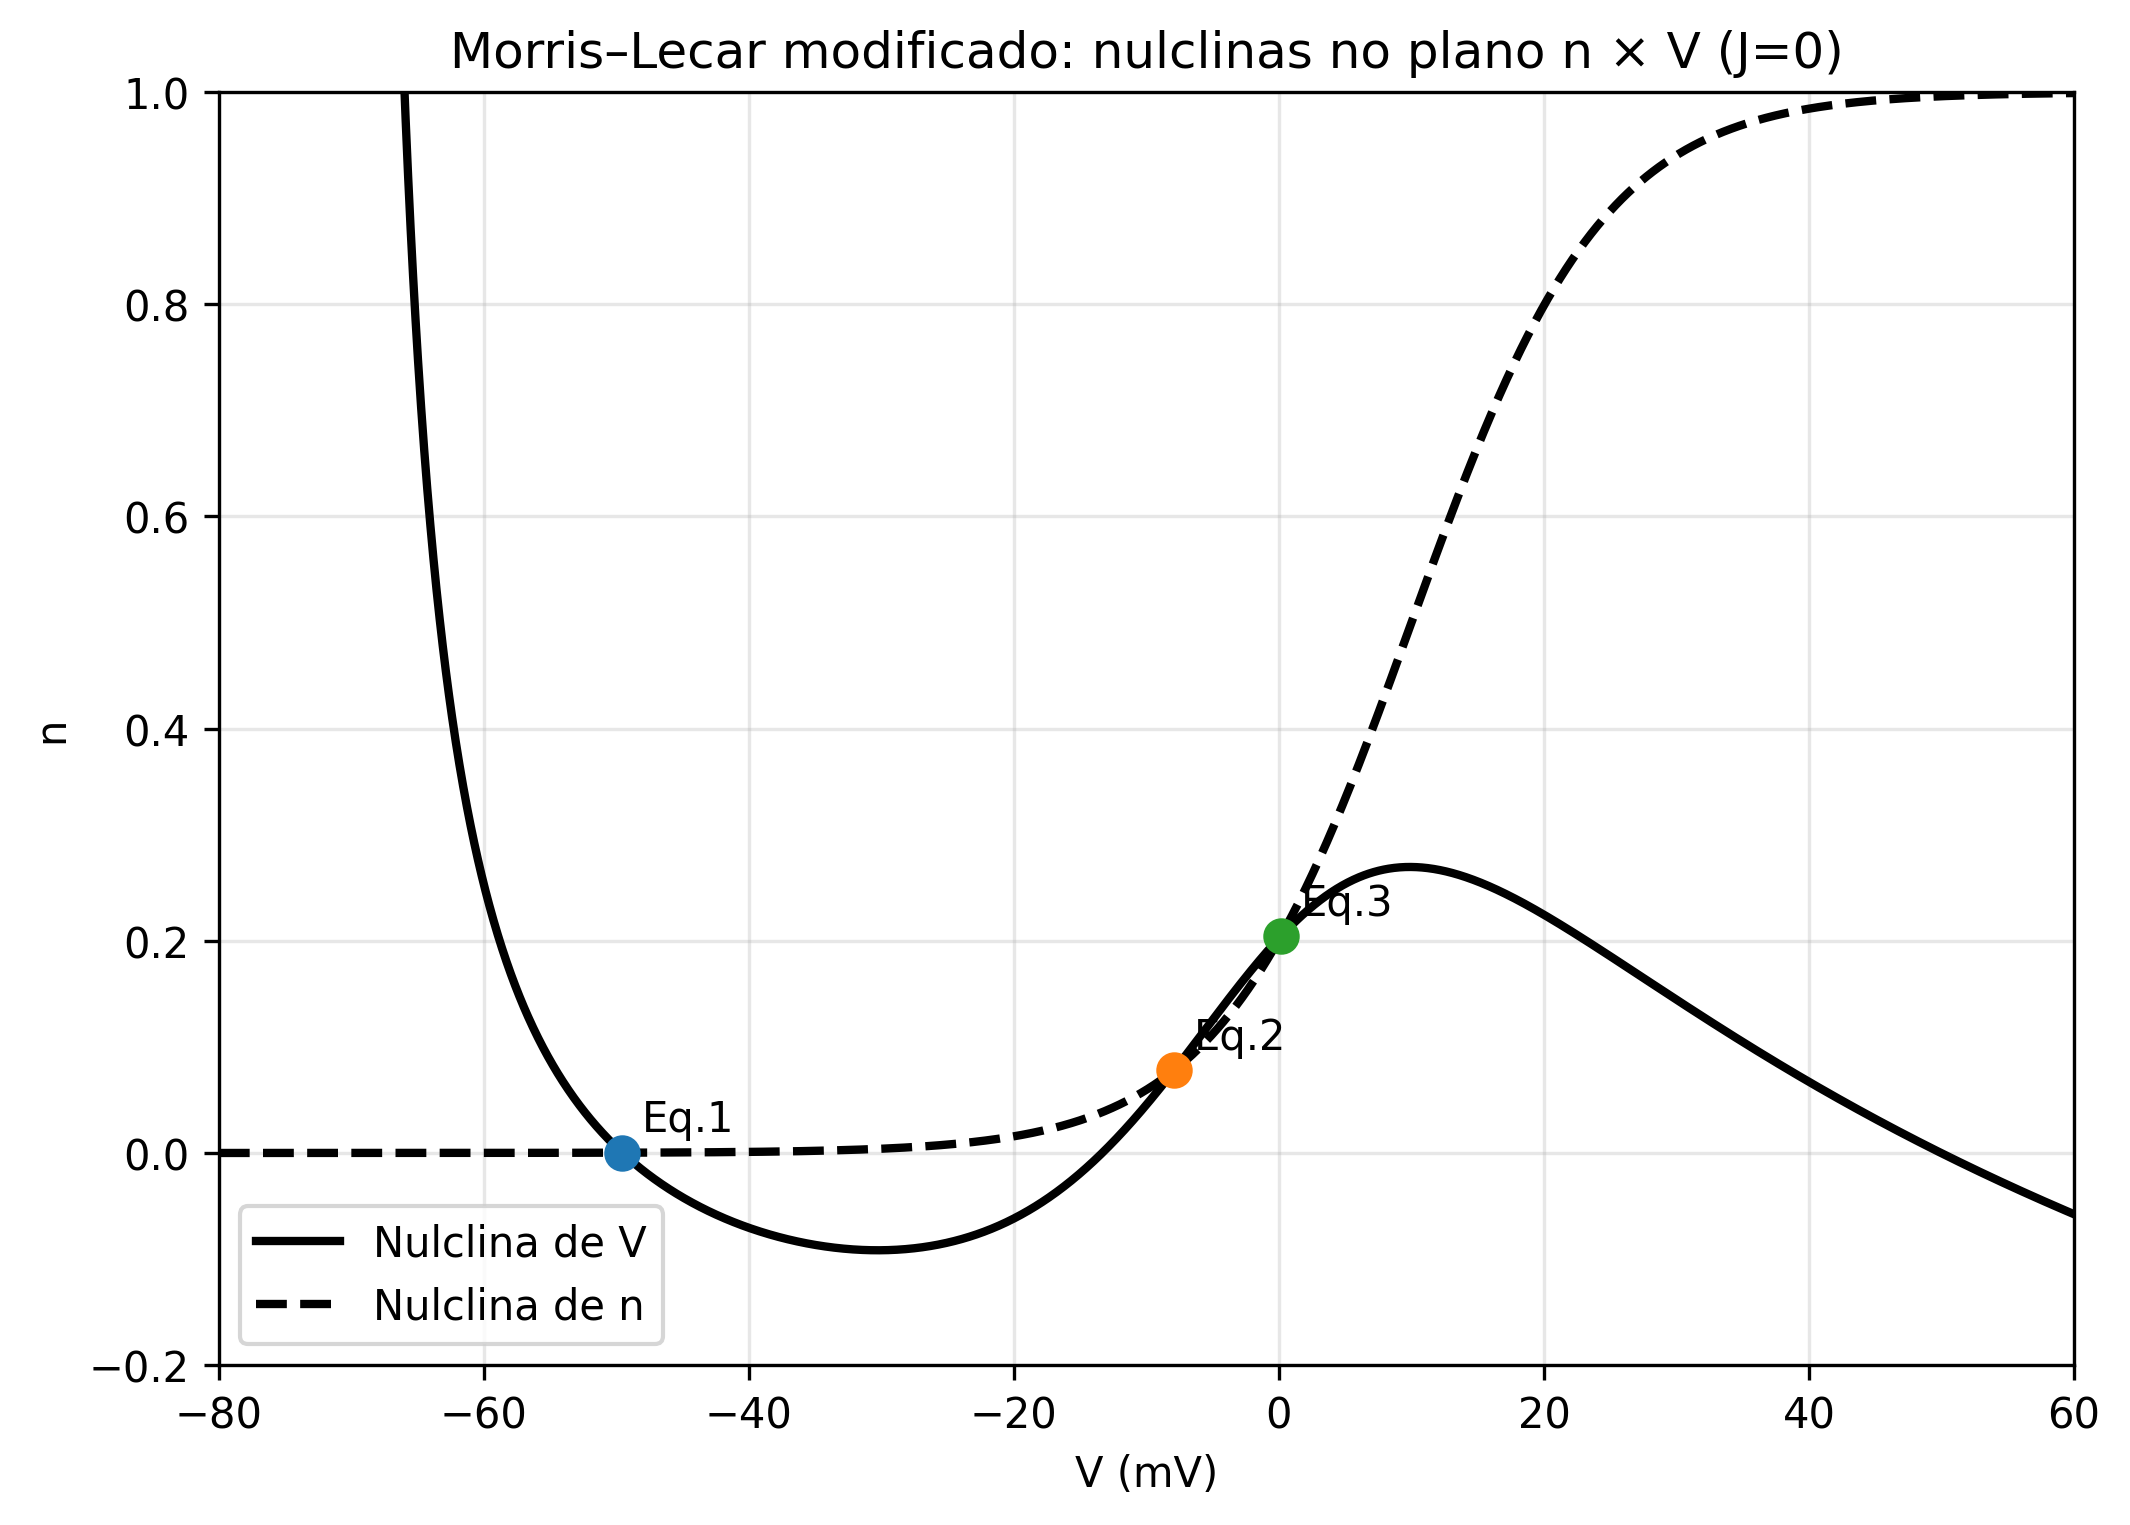
\includegraphics[width=11cm]{../figures/ex_2d.png}
		\caption{Nulclinas e pontos fixos do modelo Morris-Lecar modificado.}
	\end{figure}
	
	\noindent\textbf{(e)} Estude o efeito de pulsos instantâneos de corrente sobre o modelo de Morris-Lecar (como feito no item (b) desta questão). Para isso, simule as equações do modelo com os seguintes valores de $V_m$ como condição inicial $V_m(0)$: $-40$ mV, $-15$ mV, $-12$ mV e $-2$ mV. Use para $n(0)$ o valor de $n^*$ do ponto de equilíbrio \textit{estável} encontrado no item anterior. Faça suas simulações durarem de $t = 0$ a $t = 200$ ms. Produza três gráficos com os dados de suas simulações: (i) um gráfico com as curvas de $V_m \times t$ para os quatro valores de $v(0)$ superpostas (cada curva indicada por uma cor ou símbolo diferente); (ii) um gráfico com as curvas de $n \times t$ para os quatro valores de $v(0)$ superpostas (cada curva indicada por uma cor ou símbolo diferente); (iii) um gráfico do plano de fase $n \times V_m$ mostrando as nulclinas de $V_m$ e $n$ (em cores ou símbolos diferentes) e as trajetórias correspondentes aos quatro casos simulados (também em cores ou símbolos diferentes).\\
	
	\noindent\textbf{Resposta:}
	
	\begin{figure}[H]
		\centering
		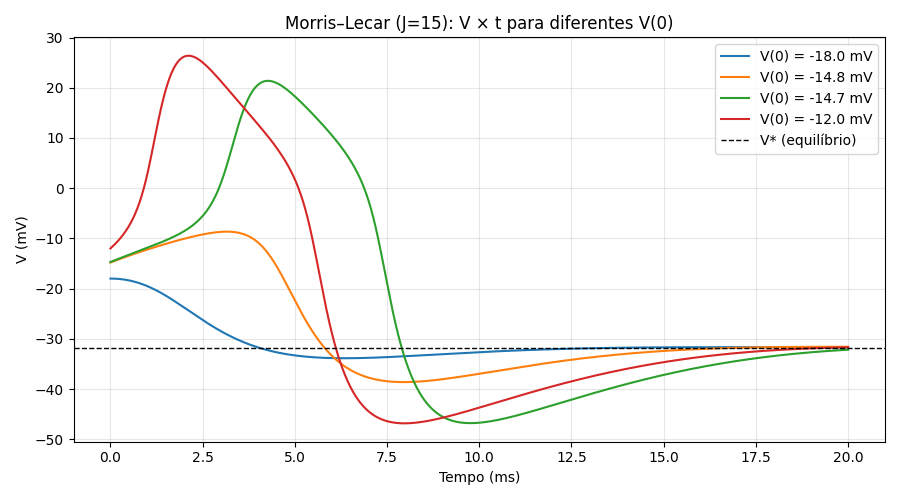
\includegraphics[width=11cm]{../figures/ex_2b_1.png}
		\caption{Gráfico de $V$ para diferentes $V(0)$ do modelo Morris-Lecar modificado.}
	\end{figure}
	
	\begin{figure}[H]
		\centering
		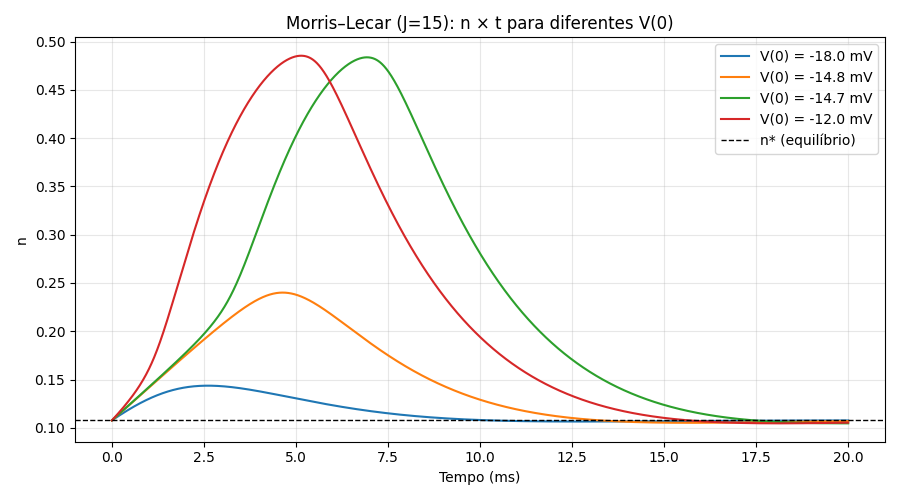
\includegraphics[width=11cm]{../figures/ex_2b_2.png}
		\caption{Gráfico de $n$ para diferentes $V(0)$ do modelo Morris-Lecar modificado.}
	\end{figure}
	
	\begin{figure}[H]
		\centering
		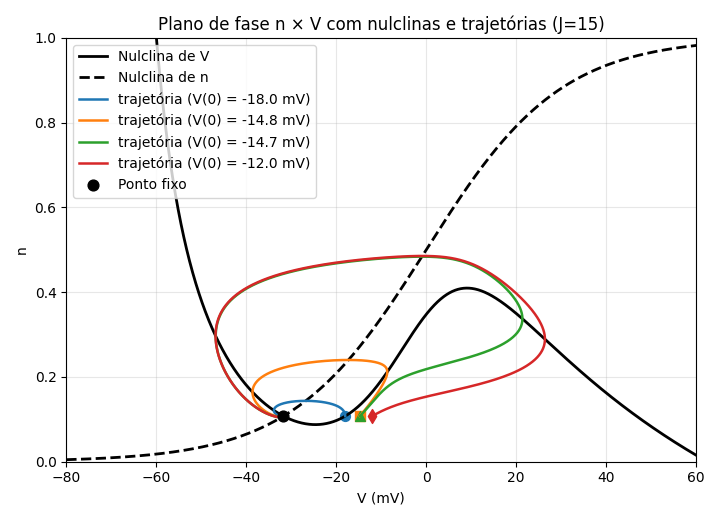
\includegraphics[width=11cm]{../figures/ex_2b_3.png}
		\caption{Plano de fase com trajetorias para diferentes $V(0)$ do modelo Morris-Lecar modificado.}
	\end{figure}
	
	\noindent\textbf{(f)} Faça uma varredura por valores de $J$ indo de $0$ a $20~\mu$A/cm$^2$ e construa a curva f–I do modelo de Morris-Lecar modificado. O modelo de Morris-Lecar modificado é de tipo I ou tipo II? Tente determinar o valor de $J$ para o qual as oscilações começam. Faça um gráfico que mostre as curvas de $V_m \times t$ superpostas (em cores ou símbolos diferentes) para três diferentes valores de $J$: $J = 7{,}9~\mu$A/cm$^2$, $J = 8{,}33~\mu$A/cm$^2$ e $J = 8{,}35~\mu$A/cm$^2$. Como o modelo de Morris-Lecar se compara com o modelo de Connor-Stevens estudado na lista 2? Para ajudar na sua resposta, construa gráficos do espaço de fase $n$–$V_m$ mostrando as nulclinas e as trajetórias do sistema para os três valores de $J$: $J = 7{,}9~\mu$A/cm$^2$, $J = 8{,}33~\mu$A/cm$^2$ e $J = 8{,}35~\mu$A/cm$^2$.\\
	
	\noindent\textbf{Resposta:}
	
	\begin{figure}[H]
		\centering
		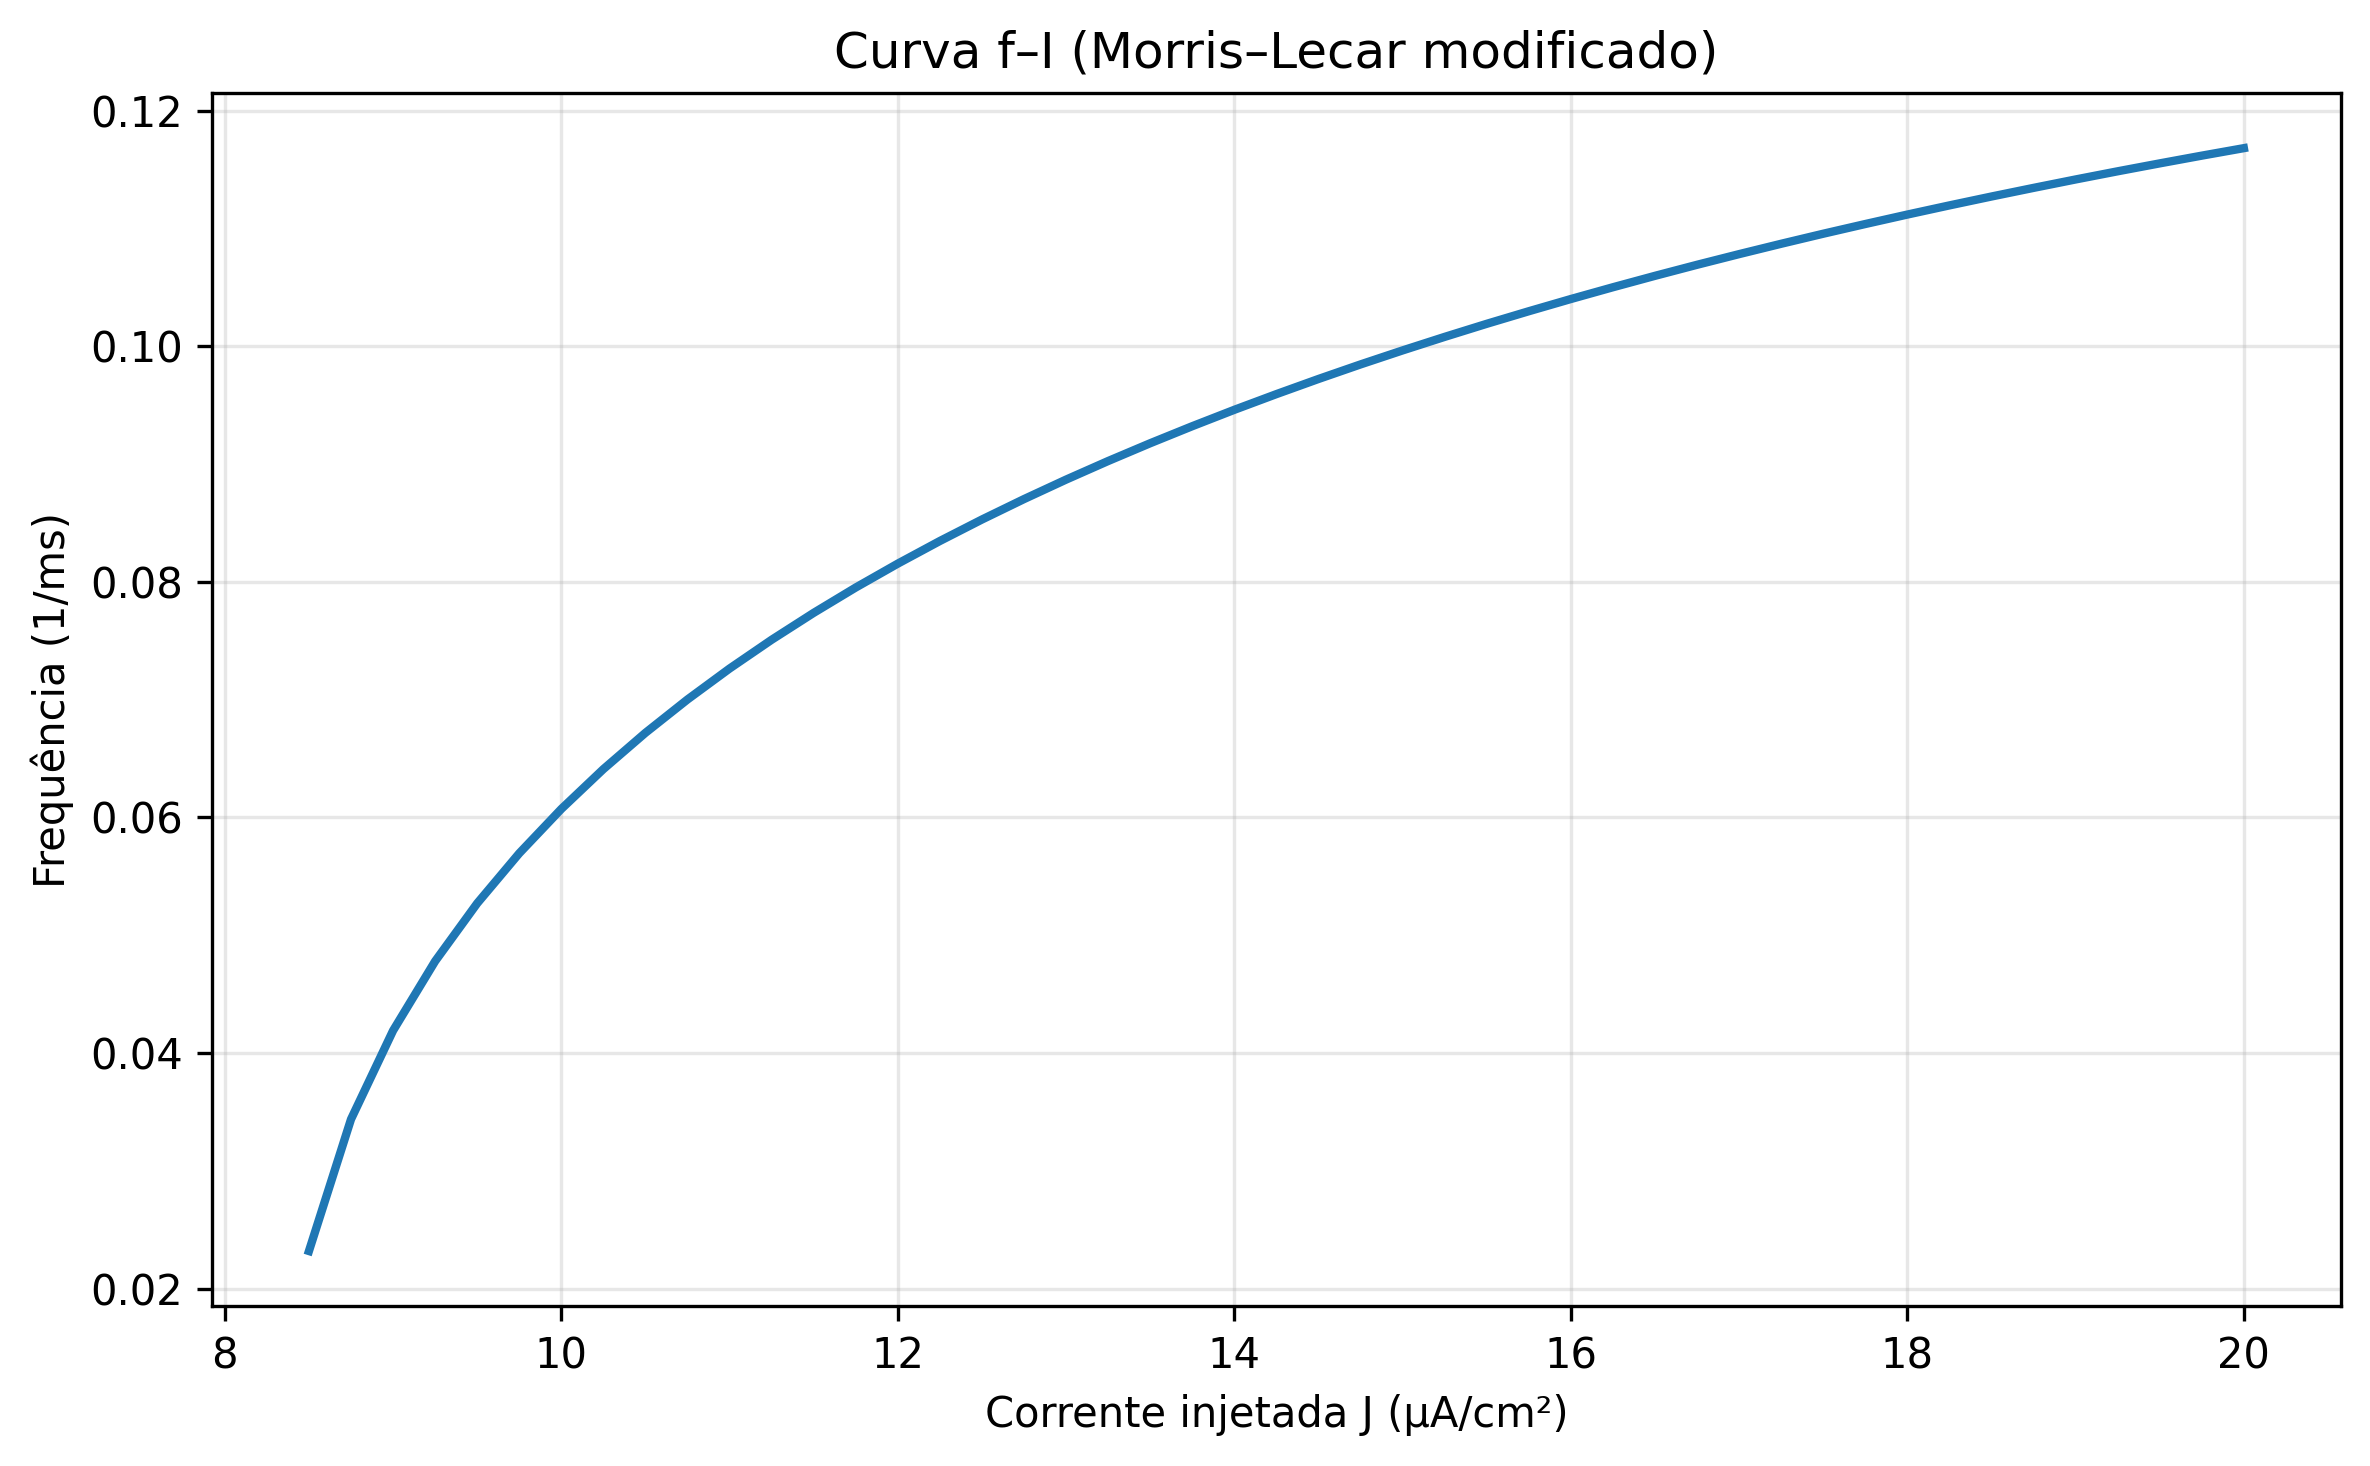
\includegraphics[width=11cm]{../figures/ex_2f_fI.png}
		\caption{Curva f-I do modelo Morris-Lecar modificado.}
	\end{figure}
	
	\begin{figure}[H]
		\centering
		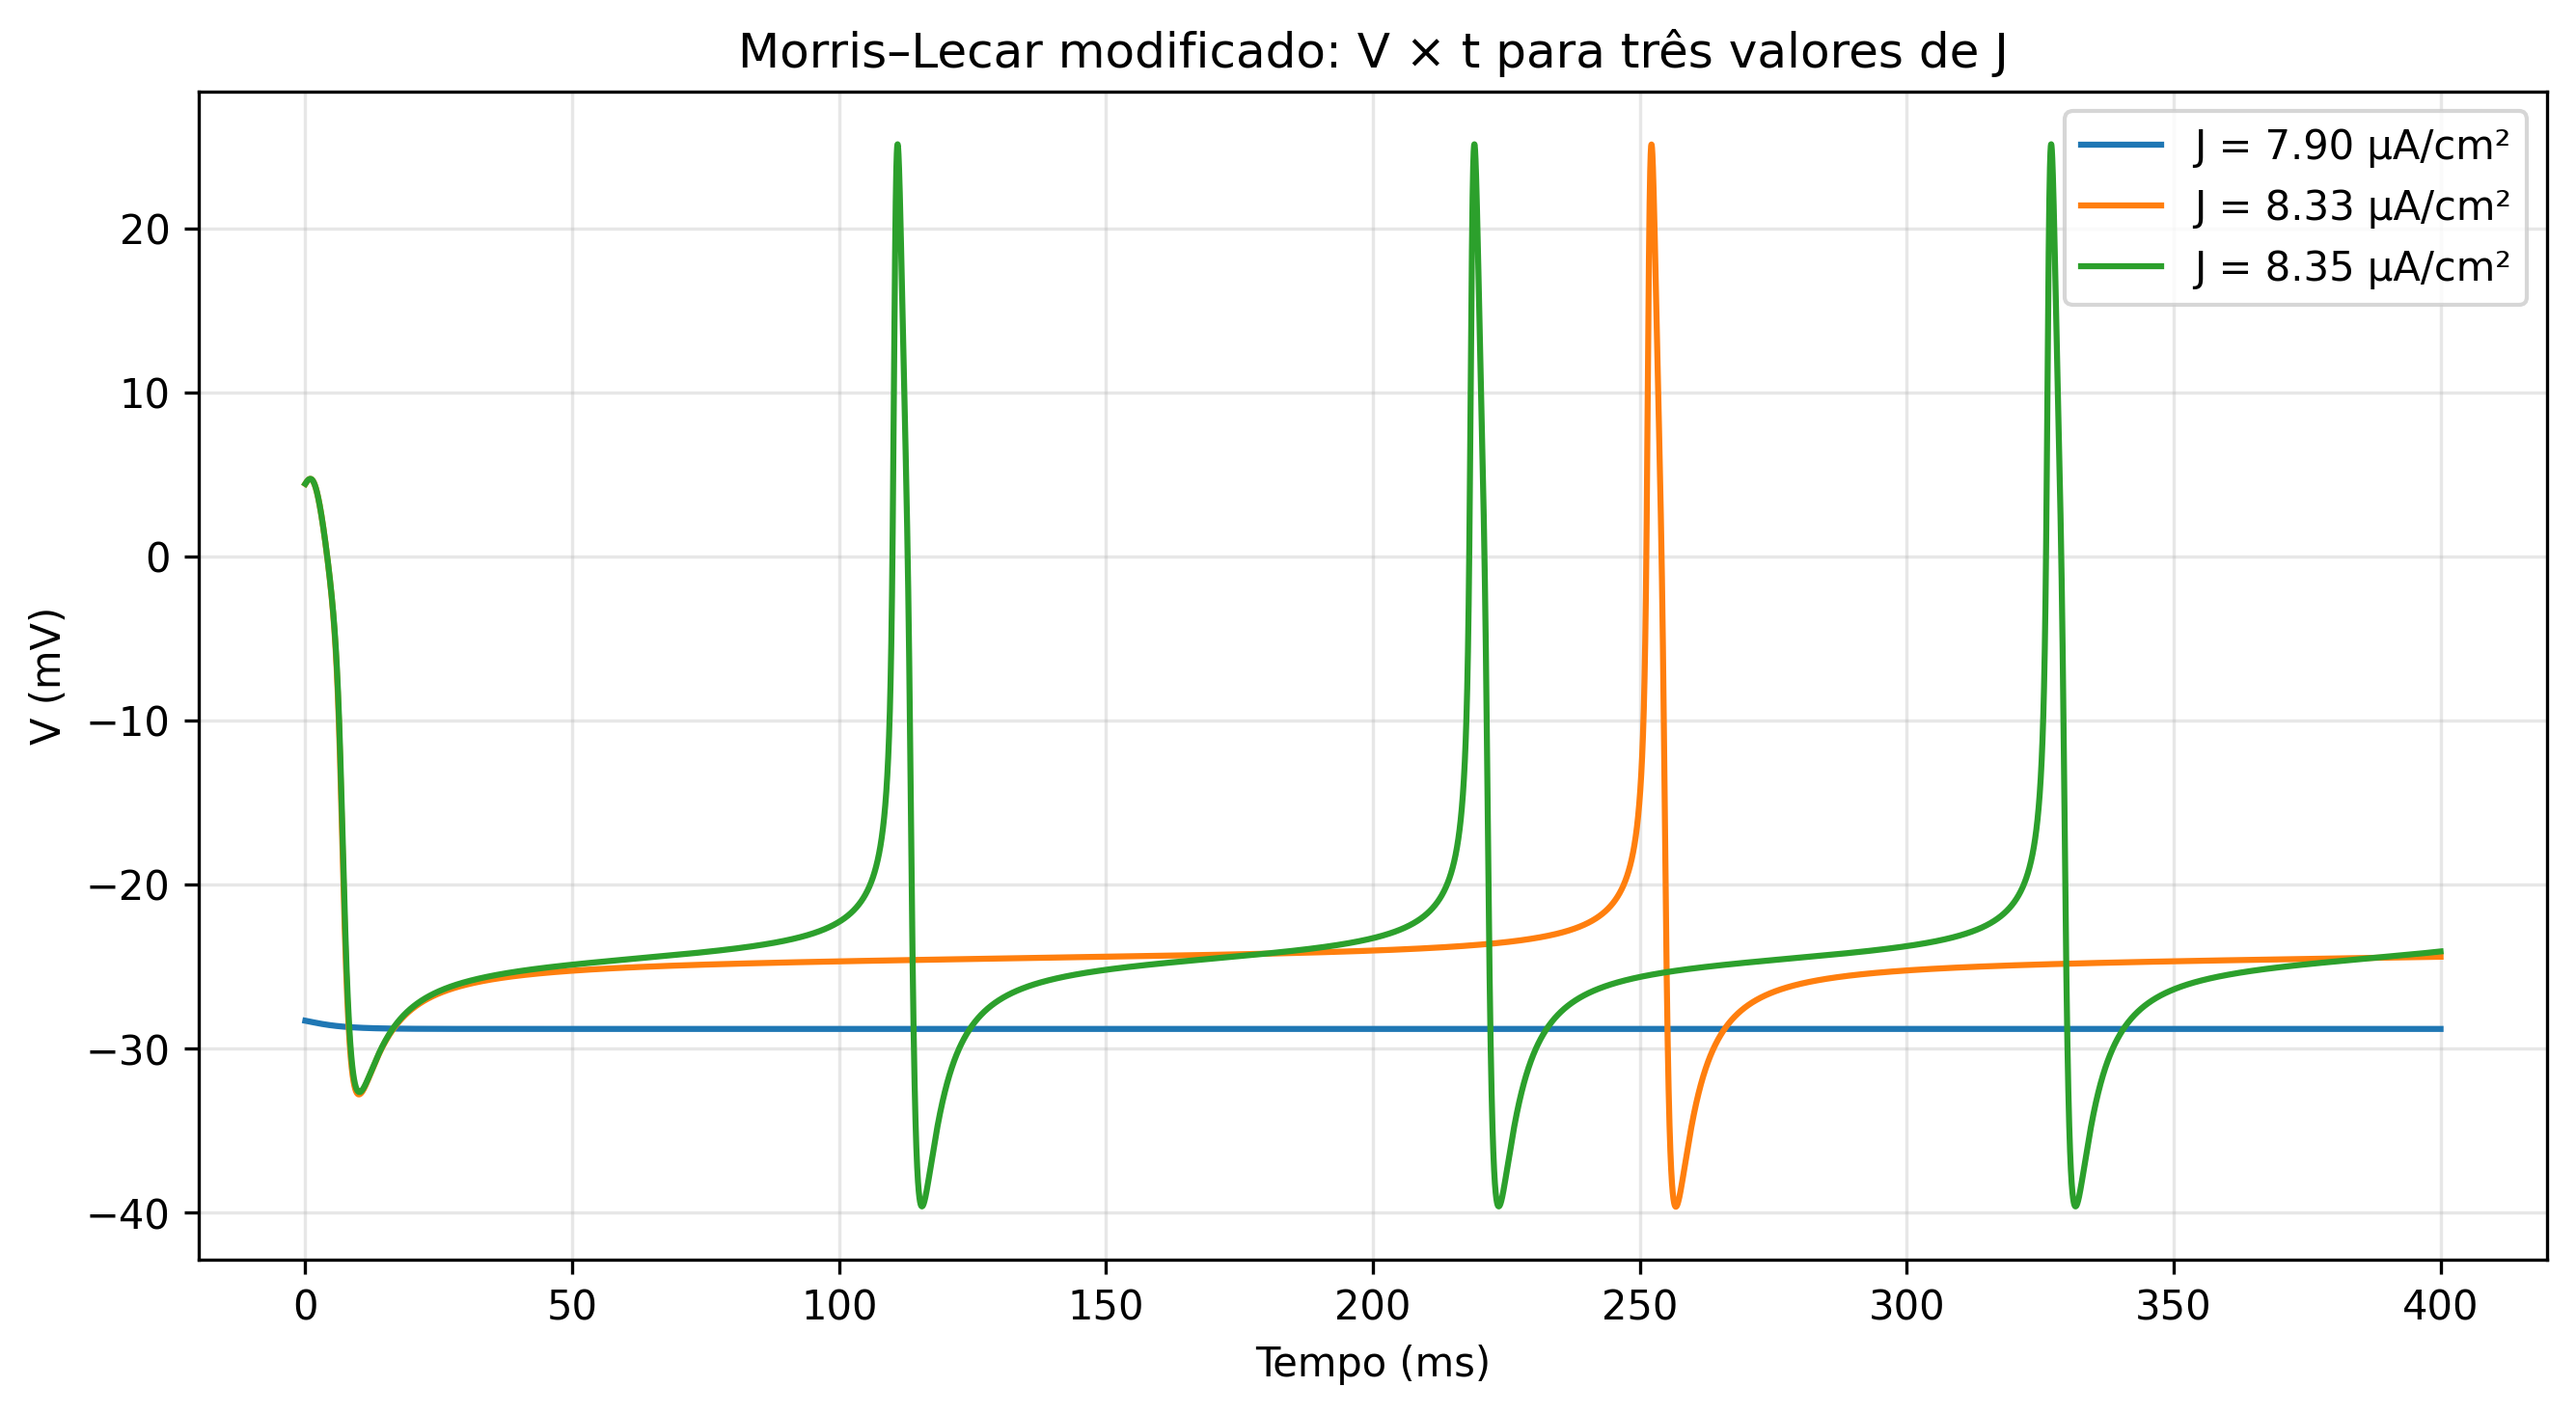
\includegraphics[width=11cm]{../figures/ex_2f_Vt.png}
		\caption{$V \times t$ para diferentes valores de $J$ do modelo Morris-Lecar modificado.}
	\end{figure}
	
	\begin{figure}[H]
		\centering
		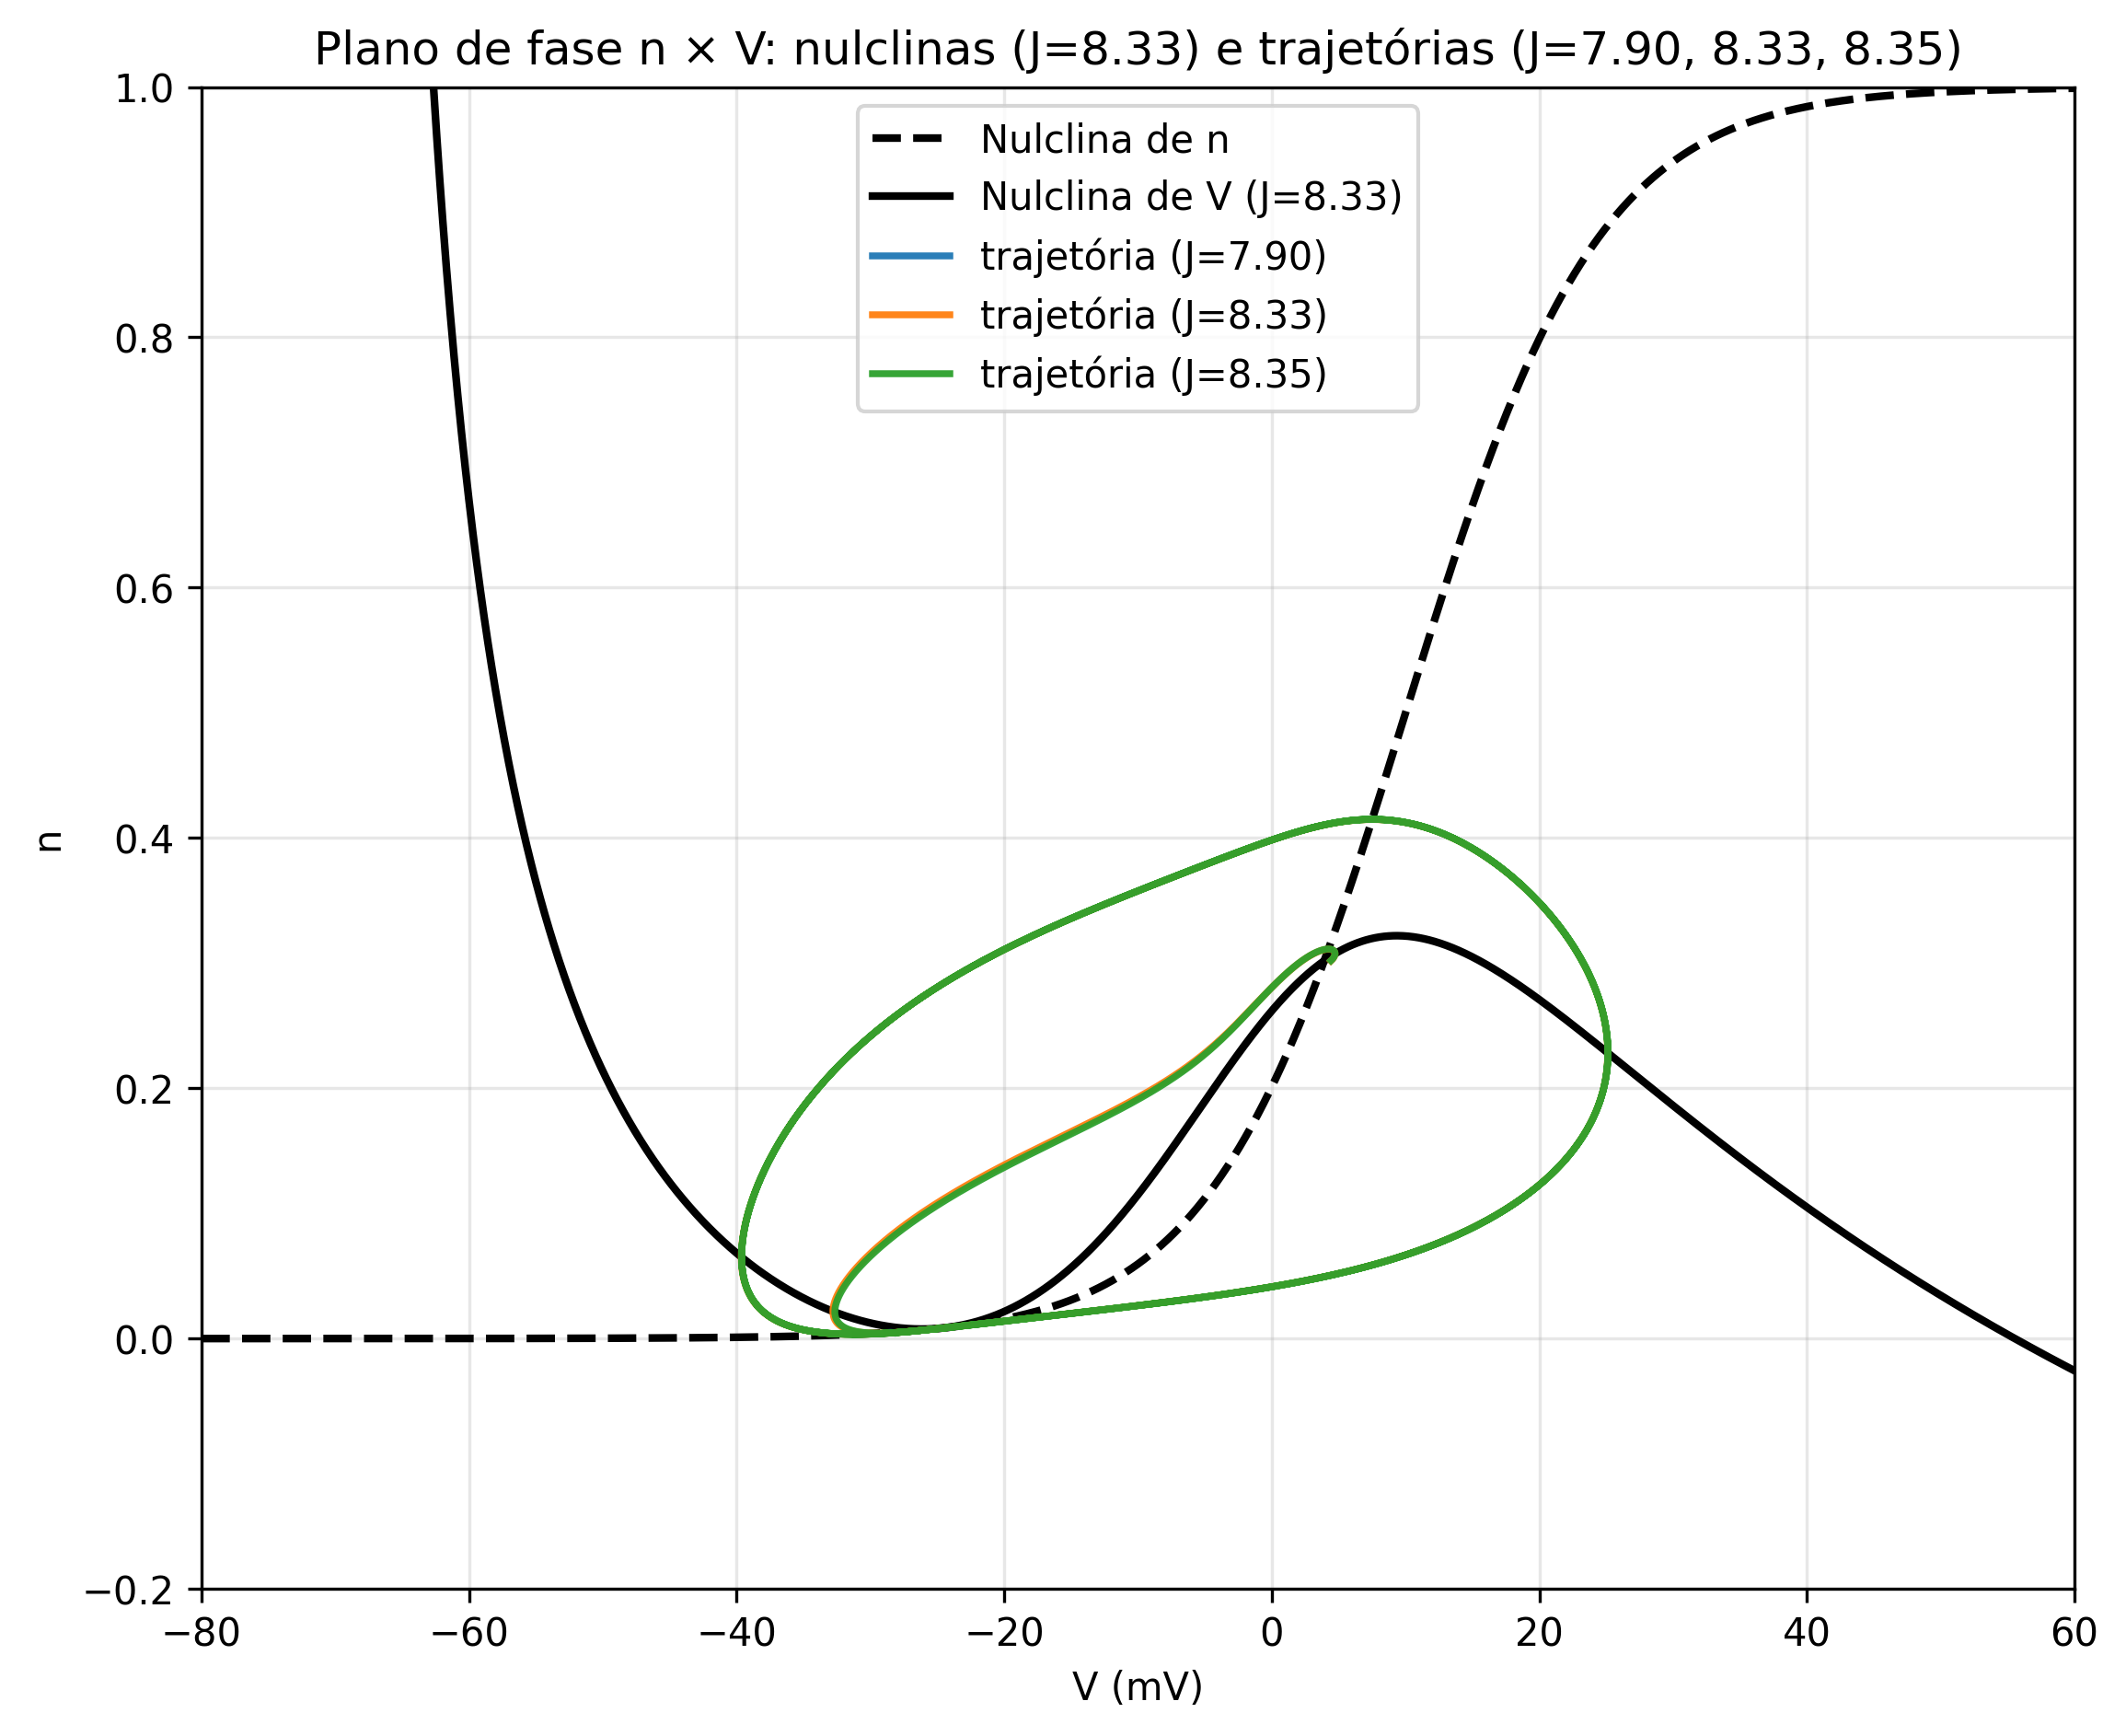
\includegraphics[width=11cm]{../figures/ex_2f_phase.png}
		\caption{Plano de fase com trajetórias do modelo Morris-Lecar modificado.}
	\end{figure}
	
	
	\noindent\textit{Curva f–I, limiar de oscilação, tipo de excitabilidade e comparação.}
	
	\medskip
	\noindent	A varredura em $J\in[0,20]\,\mu\mathrm{A/cm}^2$ mostra que a frequência permanece nula
	até um limiar e, ao ultrapassá-lo, surge com valor \emph{finito}.
	Pelos dados numéricos da f–I,
	\[
	J_c \approx 8.33\ \mu\mathrm{A/cm}^2
	\quad\text{e}\quad
	f(J_c^+)>0 .
	\]
	
	\medskip
	\noindent Como $f(J)$ \emph{não} tende a zero quando $J\to J_c^+$,
	o modelo modificado é tipo II
	
	\medskip
	\noindent Com os parâmetros usuais da lista 2, o modelo de Connor–Stevens é de tipo I. Apesar desta diferença, o modelo de Morris-Lecar modificado chega muito próximo de ser tipo I também, pois sua frequência em $J_c$ é muito baixa.
		
	
	
	
	
	
\end{document}